\documentclass[letterpaper,oneside]{book}

\usepackage{geometry}
% make full use of A4 papers
\geometry{margin=1.5cm, vmargin={0pt,1cm}}
\setlength{\topmargin}{-1cm}
\setlength{\paperheight}{29.7cm}
\setlength{\textheight}{25.1cm}

% auto adjust the marginals
\usepackage{marginfix}

\usepackage{amsfonts}
\usepackage{amsmath}
\usepackage{amssymb}
\usepackage{amsthm}
\usepackage{CJKutf8}   % for Chinese characters
\usepackage{enumerate}
\usepackage{graphicx}  % for figures
\usepackage{layout}
\usepackage{multicol}  % multiple columns to reduce number of pages
\usepackage{mathrsfs}  
\usepackage{fancyhdr}
\usepackage{subfigure}
\usepackage{tcolorbox}
\usepackage{tikz-cd}
\usepackage{gensymb}
\usepackage{upgreek}
\usepackage{dsfont}

%------------------
% common commands %
%------------------
\newcommand{\dif}{\mathrm{d}}
\newcommand{\Dim}{\mathrm{D}}
\newcommand{\avg}[1]{\left\langle #1 \right\rangle}
\newcommand{\xibold}{\boldsymbol{\xi}}
\newcommand{\varphibold}{\boldsymbol{\varphi}}
\newcommand{\psibold}{\boldsymbol{\psi}}
\newcommand{\RE}{{\text{Re}}}

% this environment is for solutions of examples and exercises
\newenvironment{solution}%
{\noindent\textbf{Solution.}}%
{\qedhere}
% the following command is for disabling environments
%  so that their contents do not show up in the pdf.
\makeatletter
\newcommand{\voidenvironment}[1]{%
  \expandafter\providecommand\csname env@#1@save@env\endcsname{}%
  \expandafter\providecommand\csname env@#1@process\endcsname{}%
  \@ifundefined{#1}{}{\RenewEnviron{#1}{}}%
}
\makeatother

%----------------------------------------
% theorem and theorem-like environments %
%----------------------------------------
\numberwithin{equation}{chapter}
\theoremstyle{definition}

\newtheorem{thm}{Theorem}[chapter]
\newtheorem{alg}[thm]{Algorithm}
\newtheorem{asm}[thm]{Assumption}
\newtheorem{axm}[thm]{Axiom}
\newtheorem{coro}[thm]{Corollary}
\newtheorem{defn}[thm]{Definition}
\newtheorem{exm}[thm]{Example}
\newtheorem{exc}[thm]{Exercise}
\newtheorem{frm}[thm]{Formula}
\newtheorem{lem}[thm]{Lemma}
\newtheorem{ntn}{Notation}
\newtheorem{prop}[thm]{Proposition}
\newtheorem{rem}{Remark}[chapter]
\newtheorem{rul}[thm]{Rule}
\newtheorem{prin}[thm]{Principle}

\begin{document}
\pagestyle{empty}
\pagenumbering{roman}

%\tableofcontents
%\clearpage

\pagestyle{fancy}
\fancyhead{}
\lhead{}
\chead{Notes on Theoretical Neuroscience}
\rhead{2022}

%\setcounter{chapter}{-1}
\pagenumbering{arabic}
% \setcounter{page}{0}

% --------------------------------------------------------
% uncomment the following to remove these environments 
%  to generate handouts for students.
% --------------------------------------------------------
%\begingroup
%\voidenvironment{rem}%
%\voidenvironment{proof}%
%\voidenvironment{solution}%

% each chapter is factored into a separate file.


\chapter{Information Theory}
\label{cha:InformationTheory}

\begin{multicols}{2}
\setlength{\columnseprule}{0.2pt}  

\section{1.1}
\label{sec:1.1}

% \begin{defn}
%   The \emph{angular momentum},
%   also called \emph{moment of momentum} $\mathbf{L}$,
%   is the cross product of a moment arm $\mathbf{r}$ and
%   the linear momentum $m \mathbf{V}$ of a fluid particle,
%   i.e.,
%   \begin{equation}
%     \mathbf{L} = \mathbf{r}\times m\mathbf{V}.
%   \end{equation}
% \end{defn}
% \begin{center}
%   \includegraphics[scale=0.45]{./png/angularMomentumDefn}
% \end{center}

\begin{prin}[Conservation of angular momentum]
  \label{prin:angularMomentum}
  The rate of change of angular momentum of a system is equal to
  the net torque acting on the system,
  i.e.,
  \begin{equation}
    \frac{\dif \mathbf{L}}{\dif t} = \boldsymbol\tau,
  \end{equation}
  where $\boldsymbol\tau$ is the torque of all external forces on the system
  about any chosen axis,
  and $\dif \mathbf{L}/\dif t$ is the rate of change of
  angular momentum of the system about the same axis.
\end{prin}

% wo ai song jian jian
% wobuai bu xi zao de songjianjian

%%% Local Variables:
%%% mode: latex
%%% TeX-master: "../notesOnFluidMechanics"
%%% End:


\documentclass[letterpaper,oneside]{book}

\usepackage{geometry}
% make full use of A4 papers
\geometry{margin=1.5cm, vmargin={0pt,1cm}}
\setlength{\topmargin}{-1cm}
\setlength{\paperheight}{29.7cm}
\setlength{\textheight}{25.1cm}

% auto adjust the marginals
\usepackage{marginfix}

\usepackage{amsfonts}
\usepackage{amsmath}
\usepackage{amssymb}
\usepackage{amsthm}
\usepackage{CJKutf8}   % for Chinese characters
\usepackage{enumerate}
\usepackage{graphicx}  % for figures
\usepackage{layout}
\usepackage{multicol}  % multiple columns to reduce number of pages
\usepackage{mathrsfs}  
\usepackage{fancyhdr}
\usepackage{subfigure}
\usepackage{tcolorbox}
\usepackage{tikz-cd}
\usepackage{gensymb}
\usepackage{upgreek}
\usepackage{dsfont}

%------------------
% common commands %
%------------------
\newcommand{\dif}{\mathrm{d}}
\newcommand{\Dim}{\mathrm{D}}
\newcommand{\avg}[1]{\left\langle #1 \right\rangle}
\newcommand{\xibold}{\boldsymbol{\xi}}
\newcommand{\varphibold}{\boldsymbol{\varphi}}
\newcommand{\psibold}{\boldsymbol{\psi}}
\newcommand{\RE}{{\text{Re}}}

% this environment is for solutions of examples and exercises
\newenvironment{solution}%
{\noindent\textbf{Solution.}}%
{\qedhere}
% the following command is for disabling environments
%  so that their contents do not show up in the pdf.
\makeatletter
\newcommand{\voidenvironment}[1]{%
  \expandafter\providecommand\csname env@#1@save@env\endcsname{}%
  \expandafter\providecommand\csname env@#1@process\endcsname{}%
  \@ifundefined{#1}{}{\RenewEnviron{#1}{}}%
}
\makeatother

%----------------------------------------
% theorem and theorem-like environments %
%----------------------------------------
\numberwithin{equation}{chapter}
\theoremstyle{definition}

\newtheorem{thm}{Theorem}[chapter]
\newtheorem{alg}[thm]{Algorithm}
\newtheorem{asm}[thm]{Assumption}
\newtheorem{axm}[thm]{Axiom}
\newtheorem{coro}[thm]{Corollary}
\newtheorem{defn}[thm]{Definition}
\newtheorem{exm}[thm]{Example}
\newtheorem{exc}[thm]{Exercise}
\newtheorem{frm}[thm]{Formula}
\newtheorem{lem}[thm]{Lemma}
\newtheorem{ntn}{Notation}
\newtheorem{prop}[thm]{Proposition}
\newtheorem{rem}{Remark}[chapter]
\newtheorem{rul}[thm]{Rule}
\newtheorem{prin}[thm]{Principle}

\begin{document}
\pagestyle{empty}
\pagenumbering{roman}

%\tableofcontents
%\clearpage

\pagestyle{fancy}
\fancyhead{}
% \lhead{Yang Li}
% \chead{Notes on Fluid Mechanics}
% \rhead{2020}

%\setcounter{chapter}{-1}
\pagenumbering{arabic}
% \setcounter{page}{0}

% --------------------------------------------------------
% uncomment the following to remove these environments 
%  to generate handouts for students.
% --------------------------------------------------------
%\begingroup
%\voidenvironment{rem}%
%\voidenvironment{proof}%
%\voidenvironment{solution}%

% each chapter is factored into a separate file.

\chapter{Neual Encoding:Firing Rates and Spike Statics}
\label{cha:Firing Rates and Spike Statics}

\begin{multicols}{2} 
\setlength{\columnseprule}{0.2pt}  

\section{Spike Trains and Firing Rate}
\label{sec:firing rate}

\subsection{Firing Rate}

\begin{asm}
  Action potentials are typically treated as identical 
  stereotyped events in neural encoding
  studies ignoring in duration, amplitude, and shape. 
  We ignore the brief duration of an action potential (about 1 ms),
  an action potential sequence can be characterized simply by a list of the
  times when spikes occurred.
\end{asm} 

\begin{ntn}
  \emph{Spike train} is represented a list of the times $\{t_i\}_{i=1}^n$ when spikes occurred.
\end{ntn}

\begin{defn}
  \emph{Neural response function} $\rho (t)$ shows whether a spike is fired at time $t$,
   which can be represent as a sum of infinitesimally narrow, 
  idealized spikes in the form of Dirac $\delta$ functions
  \begin{equation}
    \label{equ:1.1}
    \rho(t)=\sum_{i=1}^n\delta(t-t_i),
  \end{equation}
  where $t_i$ with $i=1,2,\dots,n$, recorded in the trail, is the spike train
   %taken to 
   start at time $0$ and end at time $T$, so $0\leq t_i\leq T$ for all $i$.
\end{defn}

\begin{lem}
  $\delta$ function satisfies, for any well-behaved function $h(t)$
  \begin{equation}
    \label{equ:1.3}
    \int \delta(t-\tau)h(\tau)d\tau=h(t),
  \end{equation}
  \begin{proof}
  It follows from
  \begin{equation*}
    %\lim_{\epsilon\rightarrow 0}\int_{-\infty}^{+\infty} \delta(t-\tau)h(\tau)d\tau=
    \lim_{\epsilon\rightarrow 0}\int_{t - \epsilon}^{t + \epsilon} \delta(t-\tau)h(\tau)d\tau
    =h(t)\int_{t - \epsilon}^{t + \epsilon} \delta(t-\tau)d\tau=h(t)
  \end{equation*}
  \end{proof}
which provided that the limits of the integral surround the point $t$ (if they do not,
  the integral is $0$).
\end{lem}

\begin{thm}
  $\rho(t)$ is used to re-express sums over spikes as integrals over time. For any 
  well-behaved function $h(t)$, we can write
  \begin{equation}
    \label{equ:1.2}
    \sum_{i=1}^n h(t-t_i)=\int_{-\infty}^{\infty}h(\tau)\rho(t-\tau)d\tau,
  \end{equation}
  where the integral is over the duration of the trial.
  \begin{proof}
    The equation directly follows Equation \ref{equ:1.3}.
  \end{proof}
\end{thm}

\begin{defn}
  \emph{Spike-count rate $r$} is obtained by counting the number of action potentials that appear during a trial and
  dividing by the duration of the trial,
  \begin{equation}
    r=\frac{n}{T}=\frac{1}{T}\int_0^T\rho(\tau)d\tau.
  \end{equation}
  The second equality follows from the fact that $n=\int\rho(\tau)d\tau$ and indicates
that the spike-count rate is the time average of the neural response function over the 
duration of the trial.
\end{defn}

% \begin{rem}
%   A time-dependent fring rate can be defined by counting spikes over short time intervals, but this can no longer
% be computed from a single trial values. The solution to this problem is to average over multiple trials.
% \end{rem}

\begin{rem}
  The spike-count rate can be determined from a single trial, but at the expense of 
  losing all temporal resolution about variations in the neural response during the 
  course of the trial. A time-dependent firing rate can be defined by counting spikes 
  over short time intervals, but this can no longer
be computed from a single trial.
\end{rem}

\begin{exm}
  We can define the firing rate
at time $t$ during a trial by counting all the spikes that occurred between
times $t$ and $t + \Delta t$, for some small interval $\Delta t$, and dividing this count by
$\Delta t$. However, for small $\Delta t$, which allows for high temporal resolution, the
result of the spike count on any given trial is apt to be either $0$ or $1$, giving
only two possible firing-rate values.
\end{exm}

\begin{ntn}
  We use angle brackets, $\langle\ \rangle $, to denote averages over trials that use the same stimulus.
\end{ntn}

%\begin{exm}
 % The trial-averaged neural response function is denoted by $\langle \rho(t)\rangle $
%\end{exm}

\begin{defn}
  The \emph{time-dependent firing rate} r($t$) is the the average number of spikes (averaged over trials) appearing 
  during a
  short interval between times $t$ and $t+\Delta t$, divided by the duration of
   the interval,
   \begin{equation}
    \label{equ:1.5}
     r(t)=\frac{1}{\Delta t}\int_t^{t+\Delta t}\langle \rho(\tau)\rangle d\tau,
   \end{equation}
   where $\langle\rho(t)\rangle$ is the trial-averaged neural response function.
\end{defn}      

\begin{ntn}
  We use the notation r($t$) opposed to $r$ for the spike-count rate, and use the term 
  “firing rate” without any
modifiers, we mean r($t$).
\end{ntn}

\begin{rem}
  Formally, the limit $\Delta t\rightarrow 0$ should be taken on
the right side of Equation \ref{equ:1.5}, but, in extracting a time-dependent firing
rate from data, the value of $\Delta t$ must be large enough so there are sufficient
numbers of spikes within the interval defining r($t$) to obtain a reliable estimate of the 
average.
\end{rem}

\begin{prop}
  For sufficiently small $\Delta t$, $r(t)\Delta t$ 
  is the probability of a spike occurring during a short interval of duration $\Delta t$ around the time $t$.
  %which is called \emph{spiking probablity}.
  \begin{proof}
  For sufficiently small $\Delta t$, $r(t)\Delta t$ is the average number of spikes occurring
between times $t$ and $t + \Delta t$ over multiple trials. The average number of
spikes over a longer time interval is given by the integral of $r ( t )$ over that
interval. If $t$ is small, there will never be more than one spike within the
interval between $t$ and $t + \Delta t$ on any given trial. This means that $r(t)\Delta t$ is
also the fraction of trials on which a spike occurred between those times.
\end{proof}
\end{prop}



\begin{thm}
  For any function $h$, 
  we can
replace the trial-averaged neural response function with the firing rate r($t$)
within any well-behaved integral.
  \begin{equation}
    \label{equ:1.6}
    \int h(\tau)\langle \rho(t-\tau)\rangle d\tau = \int h(\tau)r(t-\tau)d\tau.
  \end{equation}
\end{thm}

\begin{rem}
  Equation \ref{equ:1.6} establishes an important relationship between the
average neural response function and the firing rate, the two are equivalent when used inside 
integrals. And provides another interpretation of
  r($t$) as the trial-averaged density of spikes along the time axis.
\end{rem}

\begin{defn}
  \emph{Average firing rate $\langle r \rangle $} is the spike-count firing rate to be averaged over trials.
  \begin{equation}
    \label{equ:1.7}
    \langle r\rangle =\frac{\langle n\rangle }{T}
    %=\frac{1}{T}\int_{0}^{T} \langle\rho(\tau) \rangle \,d\tau =\frac{1}{T}\int_{0}^{T}r(t)\,dt
  \end{equation}
   where $\langle n \rangle $ is the trial-averaged number of the spike in the trial, 
   $T$ is the time period of the trial.
\end{defn}

\begin{prop}
  \begin{equation*}
    \langle r\rangle=\frac{1}{T}\int_{0}^{T}r(t)\,dt
  \end{equation*}
  \begin{proof}
    \begin{equation*}
      \langle r\rangle =\frac{\langle n\rangle }{T}
    =\frac{1}{T}\int_{0}^{T} \langle\rho(\tau) \rangle \,d\tau =\frac{1}{T}\int_{0}^{T}r(t)\,dt
    \end{equation*}
    The first equality indicates that $\langle r\rangle $ is just the average 
   number of spikes per trial divided by the trial duration. The third equality follows from
the equivalence of the firing rate and the trial-averaged neural response
function within integrals Equation \ref{equ:1.6}. The average firing rate is equal to
both the time average of r($t$) and the trial average of the spike-count rate $r$. 
  \end{proof}
\end{prop}

\begin{rem}
  Whenever possible, we use the terms “firing rate”, “spike-count rate”
, and “average firing rate” for r($t)$, $r$, and $\langle  r\rangle  $, respectively. In particular, 
we distinguish the spike-count rate $r$
from the time-dependent firing rate r($t$) by
including the time argument in the latter expression (unless r($t)$ is independent of time).
\end{rem}

\subsection{Measuring Firing Rates}

\begin{ntn}
  The firing rate r($t$) cannot be determined exactly from the limited data
available from a finite number of trials. In addition, there is no unique
way to approximate r($t$).
  %In order to determine firing rate r($t$), we will introduce the concept of a linear filter and kernel.
  We illustrate the methods of measuring firing rate by extracting
  firing rates from a single trial, but more accurate results could be obtained
  by averaging over multiple trials.
  \begin{exm}
    We shows $3$s of the response of a neuron in the inferotemporal cortex 
  recorded while a monkey watched a video. Neurons
  in the region of cortex where this recording was made are selective for
  complex visual images, including faces.
  \end{exm}
\end{ntn}
\begin{center}
  \label{fig:1.4A}
    \includegraphics[scale=0.048]{./png/fig:1.4A.jpg}
  \end{center}

\begin{alg}
  A simple algorithm of extracting an estimate of the firing rate from a spike train is to divide time into
discrete bins of duration $\Delta t$, count the number of spikes within each bin,
and divide by $\Delta t$.
\end{alg}

\begin{exm}
  This figure shows the approximate firing rate computed
using this procedure with a bin size of 100 ms. Note that with this procedure, the quantity being computed is 
really the spike-count firing rate over the duration of the bin, and that the firing rate 
r($t$) within a 
given bin is approximated by this spike-count rate. The binning and counting procedure 
illustrated in this figure 
generates an estimate of the firing rate that is a piecewise constant function of time, 
resembling a histogram.
\end{exm}

\begin{center}
  \label{fig:1.4B}
  \includegraphics[scale=0.053]{./png/fig:1.4B.jpg}
\end{center}

\begin{lem}
   Because spike counts can take only integer values, the rates computed by this method will 
   always 
  be integer multiples of $1 / \Delta t$, and thus they take discrete values. Decreasing 
  the value of $\Delta t$
increases temporal resolution by providing an estimate of the firing rate at
more finely spaced intervals of time, but at the expense of decreasing the
resolution for distinguishing different rates.
\end{lem}

\begin{alg}
  One algorithm to avoid quantized
firing rates is to vary the bin size so that a fixed number of spikes appears
in each bin. The firing rate is then approximated as that fixed number of
spikes divided by the variable bin width.
\end{alg}

\begin{rem}
  Counting spikes in preassigned bins produces a firing-rate estimate that
depends not only on the size of the time bins but also on their placement.
\end{rem}

\begin{alg}
To avoid the arbitrariness in the placement of bins, the algorithm is taking
a single bin or window of duration $\Delta t$ and slide it along the spike train,
counting the number of spikes within the window at each location which have a better 
temporal resolution.
\end{alg}

\begin{exm}
  \label{fig:1.4C}
  The jagged curve in  the figure below shows the result of sliding a $100$ ms wide
window along the spike train.  The firing rate approximated in 
this way
can be expressed as the sum of a window function over the times $t_i$ for
$i = 1 , 2 ,\dots, n$ when the $n$ spikes in a particular sequence occurred,
\begin{equation}
  \label{equ:1.8}
  r_{\text{approx}}(t)=\sum_{i = 1}^{n}\omega(t-t_i), 
\end{equation}
where the window function is

\begin{equation}
  \label{equ:1.9}
  \omega(t)=\left\{
    \begin{aligned}
      1/\Delta t \quad &\text{if} -\Delta t/2\leq t\leq \Delta t/2\\
      0 \quad & \text{otherwise}.
    \end{aligned}
  \right.
\end{equation}
The jagged appearance of the curve is caused 
by the discontinuous shape of the window function used.
\end{exm}

\begin{center}
  \includegraphics[scale=0.054]{./png/fig:1.4C.jpg}
\end{center}

\begin{prop}
  The sum in Equation\ref{equ:1.8} can also be written as the integral of the window
function times the neural response function
\begin{equation}
  \label{equ:1.10}
  r_{\text{approx}}(t)=\int_{-\infty}^{\infty}\omega(\tau)\rho(t-\tau)d\tau.
\end{equation}
\begin{proof}
  The proof directly follows Equation\ref{equ:1.2}.
\end{proof}
\end{prop}

\begin{defn}
  The integral in Equation \ref{equ:1.10} is called a \emph{linear filter}, and the window 
  function $\omega$, also called the \emph{filter kernel}, specifies how the neural 
  response function evaluated at time $t-\tau$ contributes to the firing rate approximated 
  at time $t$.
\end{defn}

\begin{exm}
  \label{fig:1.4D}
  Instead of the rectangular window function used in figure in example \ref{fig:1.4C}, 
  figure in example \ref{fig:1.4D} use a 
  continuous window function like the Gaussian
  \begin{equation}
    \label{equ:1.11}
    w(\tau)=\frac{1}{\sqrt{2\pi}}\sigma_{\omega}\text{exp}\left(-\frac{\tau^2}{2\sigma_{\omega}^2} \right),  
  \end{equation}
   which is used in Equation \ref{equ:1.8} generates 
a firing-rate estimate that is a smooth function of time.
In this case, $\sigma_{\omega}$  controls the temporal resolution of the resulting rate, 
playing a role analogous to $\Delta t$.
\end{exm}

\begin{center}
  \includegraphics[scale=0.245]{./png/fig:1.4D.png}
\end{center}

\begin{prin}
  A postsynaptic neuron monitoring the spike train of a presynaptic cell has
access only to spikes that have previously occurred.
\end{prin}

\begin{defn}
  A window function or kernel is called \emph{causal} when an approximation
of the firing rate at time $t$ that depends only on spikes fired before $t$ can
be calculated using a window function that vanishes when its argument is negative.

\end{defn}

\begin{defn}
  The \emph{half-wave rectification} $[z]_+$ for any quantity $z$ stands for,
\begin{equation}
  \label{equ:1.13}
  [z]_+ =\left\{
    \begin{aligned}
      z \quad &\text{if} \quad z\geqslant 0\\
      0 \quad & \text{otherwise}.
    \end{aligned}
  \right.
\end{equation}
\end{defn}

\begin{exm}
  \label{fig:1.4E}
  One commonly used window function is the $\alpha$ function
  \begin{equation}
    w(\tau)=[\alpha^2 \tau \text{exp}(-\alpha\tau) ]_+ 
  \end{equation}
  where $1/\alpha$ determines the temporal resolution of the resulting firing-rate
 estimate. The figure below shows the firing rate approximated by such a causal scheme.
\end{exm}

\begin{center}
  \includegraphics[scale=0.72]{./png/fig:1.4E.png}
\end{center}

\begin{rem}
  Note that the rate computed in example \ref{fig:1.4E} tends to peak later than the 
  rate computed in example \ref{fig:1.4D} using a temporally symmetric window function.%%这个地方需要解释一下吗?
\end{rem}

\subsection{Tuning Curve}

\begin{rem}
  Neuronal responses typically depend on many different properties of a
stimulus. In this chapter, we characterize responses of neurons as functions of 
just one of the stimulus attributes to which they may be sensitive. The value of this 
single attribute is denoted by \emph{s}. In chapter ??, we consider
more complete stimulus characterizations.
\end{rem}

\begin{defn}
  The \emph{neural response tuning curve} is the average firing rate written 
  as a function of $s$, $\langle r\rangle =f(s)$. The functional form of a tuning 
  curve depends on the parameter $s$ used to describe the stimulus. 
  %The precise choice of parameters used as arguments of tuning curve functions is partially a matter of convention.
\end{defn}

\begin{rem}
  A simple way of characterizing the response of a neuron is to count the
number of action potentials fired during the presentation of a stimulus.
This approach is most appropriate if the parameter $s$ characterizing the
stimulus is held constant over the trial. If we average the number of action potentials 
fired over (in theory, an infinite number of) trials and divide by the trial duration, 
we obtain the average firing rate, $ \langle r\rangle$, defined in Equation \ref{equ:1.7}.
\end{rem}

\begin{ntn}
  Because tuning curves correspond to firing rates, they are measured in units of spikes 
  per second or Hz.
\end{ntn}

\begin{exm}
  \label{fig:1.5}
   We show extracellular recordings of a neuron in the primary visual cortex (V1) of 
a monkey. While these recordings were being made, a
bar of light was moved at different angles across the region of the visual
field where the cell responded to light. This region is called the receptive 
field of the neuron. Note that the number of action potentials fired
depends on the angle of orientation of the bar.

The dots in the figure B of example \ref{fig:1.5} indicate the average firing rate depends on the degrees of the orientation angle of the light bar stimulus.

The data have been fitted by a response tuning curve of the form of \emph{Gaussian tuning curve}
\begin{equation}
  \label{equ:1.14}
  f(s)=r_{\text{max}}\text{exp}\left(-\frac{1}{2}\left(\frac{s-s_{\text{max}}}{\sigma_f}\right)^2\right),
\end{equation}

The curve  in figure B is a fit using
the Equation \ref{equ:1.14} with parameters $r_{\text{max}} = 52 . 14 $Hz, $s_{\text{max}}= 0 ^\circ$,
 and $\sigma_f= 14 . 73 ^\circ $,
where $s$ is the orientation angle of the light bar, $s_{\text{max}}$ is the orientation angle
evoking the maximum average response rate $r_{\text{max}}$ (with $s-s_{\text{max}} $ taken 
to lie in the range between $- 90^\circ $ and $+90^\circ$  ), and $\sigma_f$ determines the 
width of the tuning curve. The neuron responds most vigorously when a stimulus
having $s=s_{\text{max}} $ is presented, so we call $s_{\text{max}}$ the preferred orientation angle
of the neuron.

\begin{center}
  \includegraphics[scale=0.38]{./png/fig:1.5.png}
\end{center}
\end{exm}

\begin{rem}
  Tuning curves can also be measured for neurons in motor areas, in which
case the average firing rate is expressed as a function of one or more parameters describing 
a motor action.
\end{rem}

\begin{exm}
  \label{fig:1.6}
  We show an example of extracellular recordings from a neuron in primary motor cortex 
  in a monkey
  that has been trained to reach in different directions. The stacked traces for
  each direction are rasters showing the results of five different trials. The
  horizontal axis in these traces represents time, and each mark indicates
  an action potential. The firing pattern of the cell, in particular the rate at
  which spikes are generated, is correlated with the direction of arm movement.% and thus 
  encodes information about this aspect of the motor action.

  The dots in figure B of example \ref{fig:1.6} indicate the average firing rate depends 
  on the degrees of the direction of the arm movement.
  Here the data points have
  been fitted by a tuning curve in the form of a \emph{cosine tuning curve} to be half-wave 
  rectified.
\begin{equation}
    \label{equ:1.16}
    f(s)=[r_0+\left(r_{\text{max}}-r_0\right)\cos\left(s-s_{\text{max}}\right)]_+.
  \end{equation}

  where $s$ is the reaching angle of the arm, $s_{\text{max}}=161.25^\circ$ is the reaching 
  angle associated with the maximum response $r_{\text{max}}$, and $r_0=32.34$ Hz is an 
  offset or background
  firing rate that shifts the tuning curve up from the zero axis. 
  \begin{center}
    \includegraphics[scale=0.34]{./png/fig:1.6.png}
  \end{center}
\end{exm}

\begin{exm}
  \label{fig:1.7}
  The mode of retinal disparity. The gray lines with arrows show the
location on each retina of an object located nearer than the fixation point F. The
image from the fixation point falls at the fovea in each eye, the small pit where
the black lines meet the retina. The image from a nearer object falls to the left of
the fovea in the left eye and to the right of the fovea in the right eye. For objects
farther away than the fixation point, this would be reversed. The disparity angle $s$
is indicated in the figure.

The dots in figure B of example \ref{fig:1.7} indicate average firing rate of a V1 neuron depends on
retinal disparity and illustrates another important type of tuning curve.

Here the data points have been fitted with a tuning curve called
a logistic or sigmoidal function,
\begin{equation}
  \label{equ:1.17}
  f(s)=\frac{r_{\text{max}}}{1+\exp\left(\left(s_{1/2}-s\right)/\Delta_s\right)}.
\end{equation}
In this case, $s$ is the retinal disparity, the parameter $s_{1/2}$ is the disparity
that produces a firing rate half as big as the maximum value $r_{\text{max}}$ , and $\Delta_s$
controls how quickly the firing rate increases as a function of $s$. If $\Delta_s$ is
negative, the firing rate is a monotonically decreasing function of $s$ rather
than a monotonically increasing function.
\begin{center}
  \includegraphics[scale=0.39]{./png/fig:1.7.png}
\end{center}
\end{exm}

\subsection{Spike-Count Variability}
\begin{rem}
  Tuning curves allow us to predict the average firing rate, but they do not
describe how the spike-count firing rate $r$ varies about its mean value $\langle r\rangle=f(s) $ 
from trial to trial. While the map from stimulus to average
response may be described deterministically, it is likely that single-trial
responses such as spike-count rates can be modeled only in a probabilistic manner.
Generally, $r$ values can be generated from a probability
distribution with mean $f(s)$.
\end{rem}

\begin{defn}
  The trial-to-trial deviation of $r$ from $f ( s )$ is
considered to be noise, and such models are often called \emph{noise models}.
\end{defn}
\begin{defn}
  The standard deviation for the noise distribution either can be independent of 
  $f ( s )$, in which case is called \emph{additive noise}, or it can
depend on $f ( s )$. \emph{Multiplicative noise} corresponds to having the standard
deviation proportional to $f ( s )$.
\end{defn}



%\bibliography{bib/numericalApprox}
%\bibliographystyle{abbrv}
%\bibliographystyle{abbrvnat}
%\setcitestyle{authoryear,open={[},close={]}}
\end{multicols}
\end{document}


%%% Local Variables: 
%%% mode: latex
%%% TeX-master: t
%%% End: 


\section{Population Decoding}
\label{sec:Population Decoding}

\begin{rem}
  The use of large numbers of neurons to represent information is a basic
operating principles of many nervous systems. \emph{Population coding} has a
number of advantages, including reduction of uncertainty due to neuronal
variability and the ability to represent a number of different
stimulus attributes simultaneously. In the previous section, we
discussed discrimination between stimuli on the basis of the response of
a single neuron. The responses of a population of neurons can also be
used for discrimination, with the only essential difference being that terms
such as $p[r|s]$ are replaced by $p[\mathbf{r}|s]$, the conditional
probability density of the population response $\mathbf{r}$. ROC
analysis, likelihood ratio tests, and the Neyman-Pearson lemma continue to apply in exactly the same way.
\end{rem}

\begin{rem}
  \emph{Discrimination} is a special case of decoding in which only a
  few different stimulus values are considered. A more general problem
  is the extraction of a continuous stimulus parameter from one or
  more neuronal responses. In this section, we study how the value of a continuous parameter associated with a static stimulus can be decoded from the spike-count firing
rates of a population of neurons.
\end{rem}

\subsection{Encoding and Decoding Direction}
\begin{exm}
  The cercal system of the cricket, which senses the direction of incoming air
currents is an interesting example of population coding involving a
four interneurons. The figure shows average firing-rate tuning curves
for the four relevant interneurons as a function of wind
direction, which are well approximated by halfwave rectifed cosine
function. The preferred directions of the neurons are located $90^{\circ}$ from each other, and $r_{\max}$
values are typically around 40 Hz.
\end{exm}

\begin{center}
  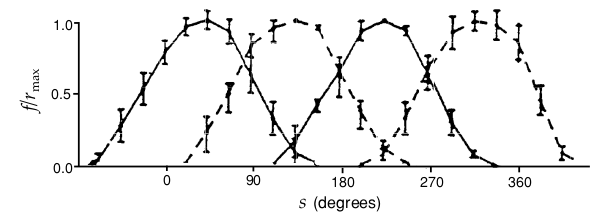
\includegraphics[scale = 0.4]{./png/3-4}
\end{center}

\begin{prop}
  \label{prop:single neuron cosine function}
  Neuron $a$ (where $a=1,2,3,4$) responds
with a maximum average firing rate when the angle of the wind direction
is $s_{a}$, the preferred-direction angle for that neuron. The tuning curve for
interneuron a in response to wind direction $s$, $\left\langle r_{a}
\right\rangle=f_a(s)$, normalized to its maximum, can be written as
\begin{equation}
  \label{eq:3.20}
  \Big( \frac{f(s)}{r_{\max}} \Big)_{a}=[(\cos(s-s_a))]_+,
\end{equation}
where the half-wave rectifcation eliminates negative firing rates. Here
$r_{\max}$, which may be different for each neuron, is a constant equal to the
maximum average firing rate.
\end{prop}

\begin{prop}
 For  the cercal system of the cricket, Equation \ref{eq:3.20} can be written as
  \begin{equation}
  \label{eq:3.21}
 \Big( \frac{f(s)}{r_{\max}} \Big)_{a}=[\vec{v}\cdot\vec{c}_a].
\end{equation}
where spatial vector $\vec{v}$ pointing parallel to the wind velocity in place of the angle
$s$ and having unit length $\big| \vec{v} \big|=1$ and a vector
  $\vec{c}_{a}$  of unit length is the preferred wind direction  pointing in the
  direction specified by the angle $s_{a}$ for each interneuron.

\begin{proof}
In this case, we can use the vector dot product to write
$\cos(s-s_a)=\vec{v}\cdot\vec{c}_a$. In terms of these
vectors, the average firing rate is proportional to a half-wave
rectified projection of the wind direction vector onto the
preferred direction axis of the neuron. And combined with the above
proposition \ref{prop:single neuron cosine function}, we give the answer.
\end{proof}

\end{prop}

\begin{rem}
  Decoding the cercal system is particularly easy because of the close relationship between the representation of wind direction it provides and a
two-dimensional Cartesian coordinate system. The preferred directions
of the four interneurons, like the $x$ and $y$ axes of a Cartesian coordinate
system, lie along two perpendicular directions. Four neurons
are required, rather than two, because firing rates cannot represent negative projections.
\end{rem}

\begin{prop}
  If $r_{a}$ is the spike-count fring rate of neuron $a$, an estimate of
  the wind direction on any given trial can be obtained from the
  direction of the vector
  \begin{equation}
    \label{eq:3.22}
    \vec{v}_{\rm{pop}}=\sum\limits_{a=1}^4\left( \frac{r}{r_{\max}} \right)_a\vec{c}_a.
  \end{equation}
  This vector is known as the \emph{population vector}, and the associated decoding
  method is called the \emph{vector method}. In fact, this encoding is
  the one that requires the least number of neurons to encode
  two-dimensional directions.
\end{prop}

\begin{exm}
In figure A, preferred directions of four cercal interneurons in relation to the
cricket’s body. The firing rate of each neuron for a fixed wind speed is proportional to the projection of the wind velocity vector $\vec{v}$ onto the preferred-direction
axis of the neuron. The projection directions
$\vec{c}_{1}$, $\vec{c}_{2}$, $\vec{c}_{3}$, and $\vec{c}_{4}$ for the four neurons
are separated by  $90^{\circ}$, and they collectively form a Cartesian coordinate system.
In figure B, the root-mean-square error in the wind direction determined by vector decoding of the firing rates of four cercal interneurons. These results were obtained
through simulation by randomly generating interneuron responses to a variety of
wind directions, with the average values and trial-to-trial variability of the firing
rates matched to the experimental data. The generated rates were then decoded
using Equation \ref{eq:3.22} and compared to the wind direction used
to generate them.
   \begin{center}
    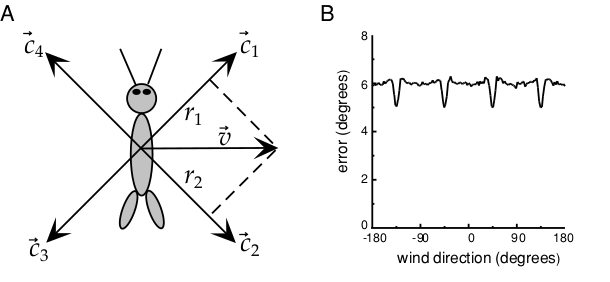
\includegraphics[scale = 0.4]{./png/3-5}
    \label{fig:3.5AB}
  \end{center}
  \end{exm}

\begin{exm}
  As discussed in chapter \ref{cha:Neural Encoding I}, tuning curves of certain neurons in the primary
motor cortex (M1) of the monkey can be described by cosine functions of
arm movement direction. Thus, a vector decomposition similar to that
of the cercal system appears to take place in M1. Many M1 neurons have
nonzero offset rates, $r_{0}$. When an arm movement is made in the direction represented by a vector of unit length, $\vec{v}$, the average fring rates for such a M1
neuron, labeled by an index $a$, can be written as
\begin{equation}
  \label{eq:3.23}
  \left( \frac{\left\langle r \right\rangle-r_{0} }{r_{\max}}\right)_{a}=\left( \frac{f(s)-r_{0}}{r_{\max}} \right)_{a}=\vec{v}\cdot\vec{c}_a,
\end{equation}
where $\vec{c}_a$ is the preferred-direction vector that defines the
selectivity of the neuron. Unlike the cercal interneurons, M1 neurons
do not have orthogonal preferred directions that form a Cartesian
coordinate system. Instead, the preferred directions of the neurons appear to point in all directions with
roughly equal probability.
\end{exm}

\begin{prop}
  If the preferred directions point uniformly in all directions and
  the number of neurons $N$ is suffciently large, the population vector
  \begin{equation}
      \label{eq:3.24}
    \vec{v}_{\rm{pop}}=\sum\limits_{a=1}^N \left( \frac{r-r_{0}}{r_{\max}} \right)_a\vec{c}_a,
  \end{equation}
will, on average, point in a direction parallel to the arm movement direction vector $\vec{c}$. If we average Equation \ref{eq:3.24} over
trials and use Equation \ref{eq:3.23}, we find
\begin{equation}
  \label{eq:3.25}
  \left\langle  \vec{v}_{\rm{pop}} \right\rangle=\sum_{a=1}^N{(\vec{v}\cdot\vec{c}_a)\vec{c}_a},
\end{equation}
 where $\vec{v}_{\rm{pop}}$ is approximately parallel
to $\vec{v}$ if a large enough number of neurons is included in the sum, and
if their preferred-direction vectors point randomly in all directions with
equal probability.
\end{prop}

\subsection{Optimal Decoding Methods}

\begin{rem}
  The vector method is a simple decoding method that can perform quite
well in certain cases, but it is neither a general nor an optimal way
to reconstruct a stimulus from the fring rates of a population of
neurons. In
this section, we dicuss two methods, that are Bayesian inference and MAP
inference, which are considered optimal by some measure.
\end{rem}

\begin{rem}
  \emph{Bayesian} and \emph{MAP} estimates use the conditional
  probability that a stimulus parameter takes a value between $s$ and
  $s+\nabla s$, given that the set of $N$ encoding neurons fired at
  rates given by $\mathbf{r}$. The probability density needed for a
  continuous stimulus parameter, $p[s|\mathbf{r}]$, can be obtained from
  the encoding probability density $p[\mathbf{r}|s]$ by the continuous version of Bayes
theorem,
\begin{equation}
  \label{eq:3.26}
  p[s|\mathbf{r}]=\frac{p[\mathbf{r}|s]p[s]}{p[\mathbf{r}]}.
\end{equation}
A disadvantage of these methods is that extracting $p[s|\mathbf{r}]$ from experimental data can be diffcult.
\end{rem}

\begin{defn}
  Below are the two optimal ways to reconstruct a stimulus from the
  fring rates of a population of neurons:
  \begin{enumerate}[(i)]
  \item The \emph{Bayesian inference} involves finding the minimum of a loss
  function $L(s,s_{\rm{bayes}})$ that quantifyes the cost of reporting
  the estimate $s_{\rm{bayes}}$ when the correct answer is $s$.
  \item  The \emph{MAP inference} chooses the stimulus value, $s_{\rm{MAP}}$,
  that maximizes the conditional probability density of the stimulus,
  $p[s_{\rm{MAP}}|\mathbf{r}]$ and \emph{ML inference} chooses
  $s_{\rm{ML}}$ to maximize the likelihood function,
  $p[\mathbf{r}|s_{\rm{ML}}]$, which generally produce estimates
  that are as accurate, in terms of the variance of the estimate, as
  any that can be achieved by a wide class of estimation methods
  (so-called unbiased estimates).
  \end{enumerate}
\end{defn}

\begin{rem}
  The value of $s_{\rm{bayes}}$ is chosen to minimize the expected
loss averaged over all stimuli for a given set of rates, that is, to minimize
the function $\int L(s,s_{\rm{bayes}})p[s|\mathbf{r}]ds$.
\end{rem}

\begin{exm}
  If the loss function is the squared difference between the estimate
  and the true value, $ L(s,s_{\rm{bayes}})=(s-s_{\rm{bayes}})^{2}$, the
  estimate that minimizes the expected loss is the mean
  \begin{equation}
    \label{eq:3.27}
    s_{\rm{bayes}}=\int p[s|\mathbf{r}]ds.
  \end{equation}
\end{exm}

\begin{exm}
 If the loss function is the absolute value of the
 difference, $L(s,s_{\rm{bayes}})=\big|s-s_{\rm{bayes}} \big|$, then
 $s_{\rm{bayes}}$ is the median rather than the mean of the
 distribution $p[s|\mathbf{r}]$.
\end{exm}


\begin{rem}
  The MAP approach is thus to choose as the estimate $s_{\rm{MAP}}$ the most
  likely stimulus value for a given set of rates. If the prior or
  stimulus probability density $p[s]$ is independent of $s$, then
  $p[s|\mathbf{r}]$ and $p[\mathbf{r}|s]$ have the same dependence on
  $s$, because the factor $p[s]/p[\mathbf{r}]$ in Equation \ref{eq:3.26} is independent of $s$. In this case, the MAP algorithm is equivalent to  maximum likelihood (ML) inference.
\end{rem}

\begin{exm}
  The root-mean-squared difference between
the true and estimated wind directions for the cercal system, using ML
and Bayesian methods is shown as follows. The Bayesian estimate in figure is based on the squared-difference loss function. Both
estimates use a constant stimulus probability density $p[s]$, so the ML and
MAP estimates are identical. The Bayesian result has a slightly
smaller average error across all angles. The dips in the error curves in figure
appear at angles where one tuning curve peaks and two others rise from
threshold. These dips are due to the two
neurons responding near threshold, not to the maximally responding neu-
ron. They occur because neurons are most sensitive at points where their
tuning curves have maximum slopes, which in this case is near threshold.
\begin{center}
  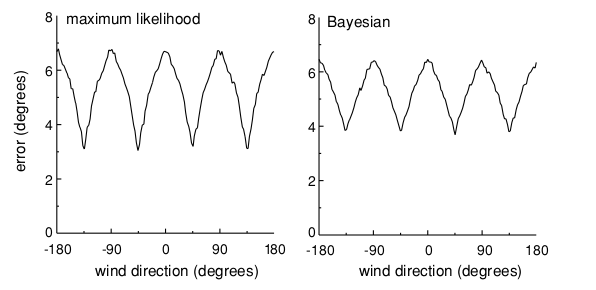
\includegraphics[scale = 0.4]{./png/3-7}
\end{center}
\end{exm}


\begin{exm}
  \label{exm:Gaussian tuning curves}
  Up to now, we have considered the decoding of a direction angle. We now
turn to the more general case of decoding an arbitrary continuous stimulus
parameter. An instructive example is provided by an array of $n$ neurons
with preferred stimulus values distributed uniformly across the full range
of possible stimulus values. An example of such an array for Gaussian
tuning curves,
\begin{equation}
  \label{eq:3.28}
  f_a(s)=r_{\rm{max}}\exp\left(-\frac{1}{2}\left(
      \frac{s-s_{a}}{\sigma_{a}} \right)^{2}\right).
\end{equation}
In this example, each neuron has a tuning curve
with a different preferred value $s_{a}$ and potentially a different
width $\sigma_{a}$. If the tuning curves are evenly and densely distributed across the range of $s$ values, the
sum of all tuning curves
$\sum f_a(s)$ is approximately independent of $s$. The roughly flat line is proportional to this sum.
\begin{center}
  \label{fig:3-8}
  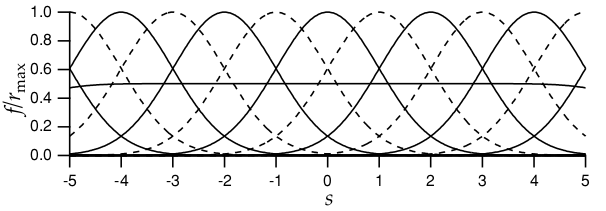
\includegraphics[scale = 0.4]{./png/3-8}
\end{center}
\end{exm}

\begin{rem}
  To implement the Bayesian, MAP, or ML approach, we need to
know the conditional firing-rate probability density $p[\mathbf{r}|s]$ that describes
this variability.
\end{rem}

\begin{prop}
  \label{prop:conditional firing-rate probability density}
  We assume that the firing rate $r_{a}$ of neuron $a$ is determined
by counting $n_{a}$ spikes over a trial of duration $T$ (so that $r_{a} = n_{a}/T$), and
that the variability can be described by the homogeneous Poisson model
discussed in chapter \ref{cha:Neural Encoding I}. In this case, the probability of stimulus s evoking
$n_{a}=r_{a}T$ spikes, when the average firing rate is $\left\langle
  r_{a} \right\rangle=f_a(s)$, is given by
\begin{equation}
  \label{eq:3.29}
  P[r_a|s]=\frac{(f_a(s)T)^{r_aT}}{(r_aT)!}\exp(-f_{a}(s)T).
\end{equation}
If we assume that each neuron fires independently, the firing-rate
probability for the population is the product of the individual
probabilities,
\begin{equation}
  \label{eq:3.30}
   P[\mathbf{r}|s]=\prod\limits_{a=1}\limits^{N}{\frac{(f_a(s)T)^{r_{a}T}} {(r_aT)!}\exp(-f_{a}(s)T)}.
\end{equation}
\end{prop}

\begin{exm}
  The filled circles in figure show a set of randomly generated firing rates
for the array of Gaussian tuning curves for $s=0$ shown above. This figure
also illustrates a useful way of visualizing population responses: plotting
the responses as a function of the preferred stimulus values. The dashed
curve is the tuning curve for the neuron with $s_{a}=0$. Because
the tuning curves are functions of $\left| s-s_{a} \right|$, the values of the dashed curve at
$s_{a}=-5,-4,\dots,5$ are the mean activities of the cells with preferred values
at those locations for a stimulus at $s=0$.
\begin{center}
    \label{fig:3-9}
  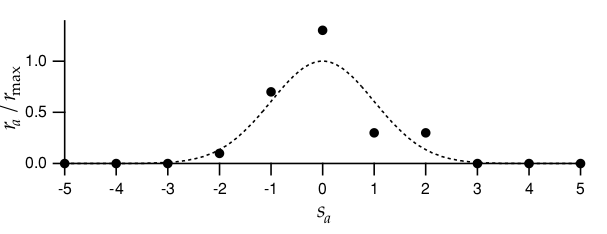
\includegraphics[scale = 0.4]{./png/3-9}
\end{center}
\end{exm}

\begin{prop}
  The ML estimated stimulus, $s_{ML}$, is the stimulus that maximizes $P[\mathbf{r}|s]$. We
find that $s_{\rm{ML}}$ is determined by
\begin{equation*}
  T\sum\limits_{a=1}\limits^{N}{r_{a}\frac{f_{a}'(s_{ML})}{f_{a}(s_{ML})}}=0,
\end{equation*}
where the prime denotes a derivative.
\begin{proof}
 To apply the ML estimation algorithm, we only need to consider the terms
in $P[\mathbf{r}|s]$ that depend on $s$. Because Equation
\ref{eq:3.30} involves a product, it is convenient to take its logarithm and write
\begin{equation}
  \label{eq:3.31}
  \ln P[\mathbf{r}|s]=T\sum\limits_{a=1}\limits^{N}{r_{a}\ln \left( f_a(s) \right)}+\dots,
\end{equation}
where the ellipsis represents terms that are independent
or approximately independent of $s$, including, as discussed above,
$\sum{f_a(s)}$.
 Setting the derivative to $0$, we give the answer.
 \end{proof}
\end{prop}

\begin{exm}
  If the tuning curves are the Gaussians of Equation \ref{eq:3.28},
  this equation can be solved explicitly using the result
  $f_{a}'(s)/f_a(s)=(s_{a}-s)/\sigma_{a}^{2}$,
    \begin{equation}
      \label{eq:3.33}
      s_{\rm{ML}}=\frac{\sum{r_as_a/\sigma_{a}^{2}}}{\sum{r_a/\sigma_{a}^{2}}}.
    \end{equation}
    If all the tuning curves have the same width, this reduces to
    \begin{equation}
      \label{eq:3.34}
      s_{\rm{ML}}=\frac{\sum{r_as_a}}{\sum{r_a}},
  \end{equation}
  which is a simple estimation formula with an intuitive interpretation as
the firing-rate weighted average of the preferred values of the encoding
neurons.
\end{exm}

\begin{rem}
  Although the stimuli obtained by maximum likelihood estimation are
  the weighted average of the best responses. This result looks very
  good, but under the influence of noise, this method may reduce the
  accuracy. The MAP algorithm allows us to include prior knowledge $p[s]$
about the distribution of stimulus values in the decoding estimate. When using
  MAP, The objective function will have one more term $\log(p[s])$
  and the maximum value can still be obtained by derivation. If the
  $p[s]$ is constant, the MAP and ML estimates are
  identical.

   Inaddition, if many neurons are observed, or if a small
  number of neurons is observed over a long trial period, even a
  nonconstant stimulus distribution has little effect and $s_{\rm{MAP}}\approx s_{\rm{ML}}$.
\end{rem}

\begin{prop}
  The MAP estimate is computed from the distribution $p[s|\mathbf{r}]$ determined by
Bayes theorem. In terms of the logarithms of the probabilities, $\ln
p[s|\mathbf{r}]=\ln p[\mathbf{r}|s]+\ln p[s]-\ln P[r]$. The last
term in this expression is independent of $s$ and can be absorbed into the ignored $s$-independent terms, so we can
write, as in Equation \ref{eq:3.31},
\begin{equation}
  \label{eq:3.35}
 \ln p[s|\mathbf{r}]=T\sum\limits_{a=1}\limits^{N}{r_{a}\ln \left(
     f_a(s) \right)+\ln p[s]+\dots}.
 \end{equation}
 Maximizing this determines the MAP estimate,
 \begin{equation}
   \label{eq:3.36}
    T\sum\limits_{a=1}\limits^{N}{\frac{r_{a}f_{a}'(s_{\rm{MAP}})}{f_{a}(s_{MAP})}}+\frac{p'[s_{\rm{MAP}}]}{p[s_{\rm{MAP}}]}=0.
 \end{equation}
\end{prop}

\begin{exm}
  If the stimulus or prior distribution is itself Gaussian with mean
  $s_{\rm{prior}}$  and
variance  $\sigma_{\rm{prior}}$ , and we use the Gaussian array of tuning curves,
Equation \ref{eq:3.36} yields
\begin{equation}
  \label{eq:3.37}
s_{\rm{MAP}}=\frac{T\sum{r_as_a}/\sigma_a^{2}+s_{\rm{prior}}/\sigma_{{\rm{prior}}}^{2}}{T\sum{r_a/\sigma_a^{2}}+1/\sigma_{{\rm{prior}}}^{2}}.
\end{equation}
\end{exm}

\begin{exm}
  The figure compares the conditional stimulus probability densities $p[s|\mathbf{r}]$
for a constant stimulus distribution (solid curve) and for a Gaussian stimulus distribution with $s_{\rm{prior}}=-2$ and $\sigma_{{\rm{prior}}}=1$, using the firing rates given
by the filled circles in last figure. If the stimulus distribution is constant,
$p[s|\mathbf{r}]$ peaks near the true stimulus value of $0$. The effect of a noncon-
stant stimulus distribution is to shift the curve toward the value $-2$, where
the stimulus probability density has its maximum, and to decrease its
width by a small amount. The estimate is shifted to the left because the
prior distribution suggests that the stimulus is more likely to take
negative values than positive ones, independent of the evoked
response. The decreased width is due to the added information that the prior distribution provides.

\begin{center}
    \label{fig:3-10}
  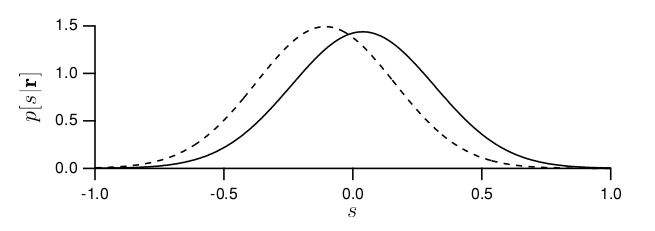
\includegraphics[scale = 0.4]{./png/3-10}
\end{center}
\end{exm}


\begin{defn}
  \label{defn:bias}
  The accuracy with which an estimate $s_{\rm{est}}$ describes a
  stimulus $s$ can be characterized by two important quantities, its
  bias $b_{\rm{est}}(s)$ and its variance
$\sigma_{\rm{est}}^{2}(s)$. The bias is the difference between the
average of $s_{\rm{est}}$ across trials that use the stimulus $s$ and the true
value of the stimulus (i.e., $s$),
\begin{equation}
  \label{eq:3.38}
  b_{\rm{est}}(s)=\left\langle s_{\rm{est}} \right\rangle-s.
\end{equation}
\end{defn}

\begin{defn}
  An estimate is termed unbiased if $b_{\rm{est}}(s)=0$ for all stimulus values.
\end{defn}

\begin{defn}
  The variance of the estimator, which quantifies how much the estimate
  varies about its mean value, is defined as
  \begin{equation}
    \label{eq:3.39}
    \sigma_{\rm{est}}^{2}(s)=\left\langle (s_{\rm{est}} -\left\langle s_{\rm{est}}  \right\rangle)^{2} \right\rangle.
  \end{equation}
\end{defn}

\begin{prop}
  The bias and variance can be used to compute the trial-average
  squared estimation error, $\left\langle (s_{\rm{est}} -s)^{2}\right\rangle$. This is a measure of the spread of the estimated values about the true value of the stimulus. Considering Definition \ref{defn:bias}, we can write the squared estimation error as
    \begin{equation}
      \label{eq:3.40}
      \left\langle (s_{\rm{est}} -s)^{2} \right\rangle=\left\langle (s_{\rm{est}} -\left\langle s_{\rm{est}}  \right\rangle+ b_{\rm{est}}(s))^{2} \right\rangle=\sigma_{\rm{est}}^{2}(s)+b_{\rm{est}}^{2}(s).
    \end{equation}
    In other words, the average squared estimation error is the sum of the
variance and the square of the bias. For an unbiased estimate, the average
squared estimation error is equal to the variance of the estimator.
\end{prop}

\begin{rem}
  In general, minimizing the decoding error in Equation
  \ref{eq:3.40} involves a trade-off between minimizing the bias and
  minimizing the variance of the estimator.
\end{rem}

\subsection{Fisher Information}
\begin{rem}
  Decoding can be used to limit the accuracy with which a neural system
encodes the value of a stimulus parameter because the encoding accuracy
cannot exceed the accuracy of an optimal decoding method.
\end{rem}

\begin{defn}
  The \emph{Fisher
information} is a quantity that provides one such measure of encoding
accuracy. Through a bound known as the \emph{Cramér-Rao bound}, the Fisher
information limits the accuracy with which any decoding scheme can extract an estimate of an encoded quantity.
\end{defn}
\begin{prop}
  The Cramér-Rao lower bound for an estimator $s_{\rm{est}}$ is based on the Cauchy-
  Schwarz inequality, which states that for any two quantities A and B,
  \begin{equation}
    \label{eq:3.67}
    \langle A^2\rangle \langle B^2\rangle\geq\langle AB\rangle^2.
    \end{equation}

\begin{proof}
 Note that
\begin{equation}
  \left\langle\left(\langle B^2\rangle A-\langle
AB\rangle B\right)^2\right\rangle\geq0
\label{eq:3.68}
\end{equation}
because it is the average value of a square. Computing the square
gives
\begin{equation}
\langle B^2\rangle^2\langle A^2\rangle-\langle AB\rangle^2\langle B^2\rangle\geq0
\label{eq:3.69}
\end{equation}
from which the inequality follows directly.
\end{proof}
\end{prop}

\begin{prop}
  The \emph{Cramér-Rao bound} limits the variance of any estimate $s_{\rm{est}}$
  according to
  \begin{equation}
    \label{eq:3.41}
     \sigma_{\rm{est}}^{2}(s)\geq \frac{\left( 1+b_{\rm{est}}'(s) \right)^{2}}{I_{\rm{F}}(s)},
   \end{equation}
   where $b_{\rm{est}}'(s)$ is the derivative of $b_{\rm{est}}(s)$ and $I_{\rm{F}}(s)$ is the Fisher
   information.

\begin{proof}
Consider the inequality of Equation \ref{eq:3.67}
   with $A=\partial \ln p/\sigma_{\rm{est}}^{2}$
   The Cauchy-Schwarz inequality then gives
\begin{equation}
\sigma_{\rm{est}}^2(s)I_F\geq\left\langle\frac{\partial \ln p[\mathbf{r}|s]}{\partial s}(s_{\rm{est}}-\langle s_{\rm{est}}\rangle)\right\rangle^2.
\label{eq:3.70}
\end{equation}
To evaluate the expression on the right side of the inequality \ref{eq:3.70}), we differentiate the defining equation for the bias (Equation \ref{eq:3.38}),
  \begin{equation}
s+b_{\rm{est}}(s)=\langle s_{\rm{est}}\rangle=\int p[\mathbf{r}|s]s_{\rm{est}}d\mathbf{r},
\label{eq:3.71}
\end{equation}
with respect to $s$ to obtain
\begin{equation}
\begin{aligned}
1+b_{\rm{est}}^{'}(s)&=\int\frac{\partial p[\mathbf{r}|s]}{\partial s}s_{\rm{est}}d\mathbf{r}\\
&=\int p[\mathbf{r}|s]\frac{\partial\ln p[\mathbf{r}|s]\partial}{\partial s}s_{\rm{est}}d\mathbf{r}\\
&=\int p[\mathbf{r}|s]\frac{\partial\ln p[\mathbf{r}|s]\partial}{\partial s}(s_{\rm{est}}-\langle s_{\rm{est}}\rangle).
\end{aligned}
\label{eq:3.72}
\end{equation}
The last equality follows from the identity
\begin{equation}
\int p[\mathbf{r}|s]\frac{\partial\ln p[\mathbf{r}|s]}{\partial s}\langle s_{\rm{est}}\rangle d\mathbf{r}=\langle s_{\rm{est}}\rangle\int\frac{\partial p[\mathbf{r}|s]}{\partial s}d\mathbf{r}=0,
\label{eq:3.73}
\end{equation}
because $\int p[\mathbf{r}|s]d\mathbf{r}=1$. The last line of equation  \ref{eq:3.72} is just another way
of writing the expression being squared on the right side of the inequality
\ref{eq:3.70}, so combining this result with the inequality gives
\begin{equation}
\sigma_{\rm{est}}^2(s)I_F\geq(1+b_{\rm{est}}^{'}(s))^2,
\label{eq:3.74}
\end{equation}
which, when rearranged, is the Cramér-Rao bound of Equation \ref{eq:3.41}.
\end{proof}
\end{prop}

\begin{prop}
  If we assume here that the firing rates take continuous values and
  that their distribution in response to a stimulus $s$ is described
  by the conditional probability density $p[\mathbf{r}|s]$(assuming
  the latter is sufficiently smooth) by, $I_{\rm{F}}(s)$ can be written as
\begin{equation}
  \label{eq:3.42}
  I_{\rm{F}}(s)=\left\langle
    -\frac{\partial^{2}\ln p[\mathbf{r}|s]}{\partial s^{2}}
  \right\rangle=\int p[\mathbf{r}|s]\left( -\frac{\partial^{2}\ln p[\mathbf{r}|s]}{\partial s^{2}} \right)d\mathbf{r},
\end{equation}
We can verify that the Fisher information can also be written as
\begin{equation}
  \label{eq:3.43}
  \left\langle \left( \frac{\partial\ln p[\mathbf{r}|s]}{\partial s} \right)^{2}
  \right\rangle=\int p[\mathbf{r}|s]\left( \frac{\partial\ln p[\mathbf{r}|s]}{\partial s} \right)^{2}d\mathbf{r}.
\end{equation}
\end{prop}

\begin{rem}
  As Equation \ref{eq:3.42} shows, the Fisher information is a measure of the expected curvature of the log likelihood at the stimulus value
$s$. Curvature is important because the likelihood is expected to be at
a maximum near the true stimulus value $s$ that caused the
responses. Therefore, we can get two cases:
\begin{enumerate}[(i)]
\item If the likelihood is very curved, and thus the Fisher information is
large, responses typical for the stimulus $s$ are much less likely to
occur for slightly different stimuli. Therefore, the typical response
provides a strong indication of the value of the stimulus.
\item If the
likelihood is fairly flat, and thus the Fisher information is small,
responses common for $s$ are likely to occur for slightly different
stimuli as well. Thus, the response does not as clearly determine the stimulus value.
\end{enumerate}
\end{rem}

\begin{rem}
  The Fisher information is purely local in the sense that it
does not reflect the existence of stimulus values completely different from
$s$ that are likely to evoke the same responses as those evoked by $s$ itself.
\end{rem}

\begin{rem}
  The Cramér-Rao bound sets a limit on the accuracy of any unbiased estimate of the stimulus. When $b_{\rm{est}}(s)=0$, Equation
\ref{eq:3.40} indicates that the average squared estimation error is
equal to $\sigma_{\rm{est}}^{2}$ and, by Equation \ref{eq:3.41}, this
satisfies the bound $\sigma_{\rm{est}}^{2} \geq
1/I_{\rm{F}}(s)$. Provided that we restrict ourselves to unbiased
decoding schemes, the Fisher information sets an absolute limit on
decoding accuracy, and it thus provides a useful limit on encoding
accuracy. In some cases, biased schemes may produce more accurate
results than unbiased ones. For a biased estimator, the average
squared estimation error and the variance of the estimate are not
equal, and the estimation error can be either larger or smaller than $1/I_{\rm{F}}(s)$ .
\end{rem}

\begin{rem}
  The limit on decoding accuracy set by the Fisher information can be
  attained by a decoding scheme we have studied, the maximum
  likelihood method. In the limit of large numbers of encoding
  neurons, and for most firing-rate distributions, the ML estimate is unbiased and saturates the
Cramér-Rao bound.
\end{rem}

\begin{defn}
  \label{defn:efficient estimator}
  Any unbiased estimator that saturates the Cramér-Rao lower bound is
  called efficient, i.e.
  \begin{equation}
    \sigma_{\rm{est}}^{2} =1/I_{\rm{F}}(s).
  \end{equation}
\end{defn}
\begin{thm}
 $I_{\rm{F}}(s)$ grows linearly with $N$, and the ML estimate obeys a
central limit theorem, so that $N^{1/2}(s_{\rm{ML}}-s)$ is Gaussian
distributed with a variance that is independent of $N$ in the large
$N$ limit. In the limit
$N \rightarrow \infty$, the ML estimate is asymptotically consistent, in the sense that
$P[|s_{\rm{ML}}-s|>\varepsilon]\rightarrow 0$ for any $\varepsilon >0$.
\end{thm}

\begin{exm}
  The Fisher information for a population of neurons with uniformly
  arrayed tuning curves (the Gaussian array in example \ref{exm:Gaussian tuning curves} for example) and
Poisson statistics can be computed from the conditional firing-rate probability in Equation \ref{eq:3.31}. Because the spike-count rate is
described here by a probability rather than a probability density, we
use the discrete analog of Equation \ref{eq:3.42},
\begin{equation}
  \label{eq:3.44}
  I_{\rm{F}}(s)=\left\langle
    -\frac{\partial^{2}\ln p[\mathbf{r}|s]}{\partial s^{2}}
  \right\rangle=T\sum\limits_{a=1}\limits^N {\left\langle r_{a} \right\rangle{\left(\left( \frac{f_a'(s)}{f_a(s)} \right)^{2}-\frac{f_a''(s)}{f_a(s)}\right)}}.
  \end{equation}
If we assume that the array of tuning curves is symmetric, like the Gaussian array in example \ref{exm:Gaussian tuning curves}, the second term
in the parentheses of the last expression sums to $0$. We can also
make the replacement $\left\langle r_{a}
\right\rangle=f_a(s)$, producing the final result
\begin{equation}
  \label{eq:3.45}
  I_{\rm{F}}(s)=T\sum\limits_{a=1}\limits^N \frac{f_a'(s)^{2}}{f_a(s)}.
\end{equation}
In this expression, each neuron contributes an amount to the Fisher
information proportional to the square of its tuning curve slope and inversely
proportional to the average firing rate for the particular stimulus value being estimated.
\end{exm}

\begin{exm}
  The Fisher information for a single neuron with a Gaussian tuning
curve with $s=0$ and $\sigma_a=1$, and Poisson variability. The Fisher information (solid
curve) has been divided by $r_{\max}T$, the peak firing rate of the tuning curve times
the duration of the trial. The dashed curve shows the tuning curve scaled by $r_{\max}$.
Note that the Fisher information is greatest where the slope of the tuning curve is
highest, and vanishes at $s=0$, where the tuning curve peaks.

\begin{center}
  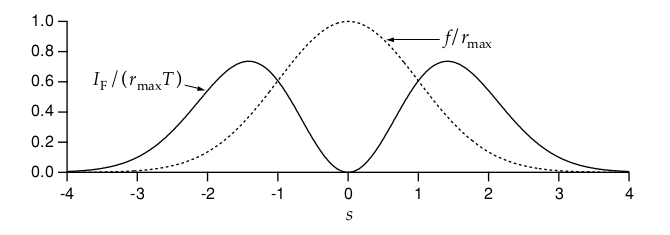
\includegraphics[scale = 0.4]{./png/3-11}
\end{center}
\end{exm}

\begin{rem}
  Individual neurons carry the most Fisher
information in regions of their tuning curves where average firing rates
are rapidly varying functions of the stimulus value, not where the firing
rate is highest.
\end{rem}
\begin{rem}
   The Fisher information can be used to derive an interesting result on the
optimal widths of response tuning curves. Consider a population of neurons with tuning curves of identical shapes, distributed evenly over a
range of stimulus values as in Example \ref{exm:Gaussian tuning curves}. Equation \ref{eq:3.45} indicates that the
Fisher information will be largest if the tuning curves of individual neurons are rapidly varying (making the square of their derivatives large), and
if many neurons respond (making the sum over neurons large). For typical neuronal response tuning curves, these two requirements are in conflict.
If the population of neurons has narrow tuning curves,
individual neural responses are rapidly varying functions of the stimulus,
but few neurons respond. Broad tuning curves allow many neurons to
respond, but the individual responses are not as sensitive to the stimulus
value.
\end{rem}
\begin{exm}
  To determine whether narrow or broad tuning curves produce the
more accurate encodings, we consider a dense distribution of Gaussian
tuning curves, all with $\sigma_a=\sigma_{r}$. Using such curves in
Equation \ref{eq:3.45}, we find
\begin{equation}
  \label{eq:3.46}
  I_{\rm{F}}(s)=T\sum\limits_{a=1}\limits^N
  {\frac{r_{\max}(s-s_{a})^{2}}{\sigma_r^{4}}\exp \left( -\frac{1}{2}\left( \frac{s-s_{a}}{\sigma_{r}} \right)^{2} \right)}.
\end{equation}
\end{exm}

\begin{prop}

This expression can be approximated by replacing the sum over neurons
with an integral over their preferred stimulus values and multiplying by a
density factor $\rho_{s}$. The factor $\rho_{s}$ is the density with which the neurons cover
the range of stimulus values, and it is equal to the number of neurons with
preferred stimulus values lying within a unit range of $s$ values. Replacing
the sum over $a$ with an integral over a continuous preferred stimulus parameter $\xi$ (which replaces $s_{a}$ ), we find
\begin{equation}
  \begin{aligned}
    \label{eq:3.47}
   I_{\rm{F}}(s)&=\rho_{s}T\int_{-\infty}^{\infty}{\frac{r_{\max}(s-\xi)^{2}}{\sigma_r^4}\exp\left(-\frac{1}{2}\left( \frac{s-\xi}{\sigma_r}\right)^{2} \right)}\\
                  &=\frac{\sqrt{2\pi}\rho_{s}\sigma_rr_{\max}T}{\sigma_r^2}.
  \end{aligned}
\end{equation}
The number of neurons that respond to a given stimulus value is
roughly $\rho_{s}\sigma_r$, and the Fisher information is proportional to this number divided by the square of the
tuning curve width seen from Equation \ref{eq:3.47}.Combining these factors, the Fisher information is inversely proportional to $\sigma_{r}$, and the encoding accuracy increases with narrower tuning curves.
\end{prop}

\begin{prop}
  Consider a stimulus with
$D$ parameters and suppose that the response tuning curves are products
of identical Gaussians for each of these parameters. If the tuning curves
cover the $D$-dimensional space of stimulus values with a uniform density $\rho_{s}$, the number of responding neurons for any stimulus value is proportional to $\rho_{s}\sigma_r^{D}$ and, using the same integral approximation as in equation (\ref{eq:3.47}), the Fisher information is
\begin{equation}
  I_{\rm{F}}=\frac{(2\pi)^{D/2}D\rho_{s}\sigma_r^{D}r_{\max}T}{\sigma_r^2}=(2\pi)^{D/2}D\rho_{s}\sigma_r^{D-2}r_{\max}T.
\end{equation}
\end{prop}

\begin{rem}
  The trade-off between the encoding accuracy of individual neurons and the
number of responding neurons depends on the dimension of the stimulus space. Narrowing the tuning curves (making $\sigma_{r}$ smaller) increases the
Fisher information for $D=1$, decreases it for $D > 2$, and has no impact if
$D = 2$.
\end{rem}

\subsection{Optimal Discrimination}
\begin{rem}
   In the first part of this chapter, we considered discrimination between two
values of a stimulus. An alternative to the procedures discussed there is
simply to decode the responses and discriminate on the basis of the estimated stimulus values.
\end{rem}
\begin{prop}
  Consider the case of discriminating between s
and $s+\Delta s$ for small $\Delta s$. For large $N$, the average value of the difference
between the ML estimates for the two stimulus values is equal to
$\Delta s$ (because the estimate is unbiased) and the variance of each estimate (for small
$\Delta s$) is $1/I_{\rm{F}}(s)$ . Thus, the discriminability, defined
in Equation \ref{eq:3.4}, for the ML-based test is
\begin{equation}
  \label{eq:3.49}
  d'=\Delta s \sqrt{I_{\rm{F}}(s)}.
\end{equation}
It can be known that the larger the Fisher information, the higher the discriminability.
\end{prop}

\begin{exc}
  Proof that for small $s$, this discriminability is the same
as that of the likelihood ratio test $Z(\mathbf{r})$ defined in Equation \ref{eq:3.47}.
\end{exc}



\begin{exm}
  The figure makes a comparison of Fisher information and discrimination thresholds for
orientation tuning.The solid curve is the minimum standard deviation of an estimate of orientation angle from the Cramér-Rao bound, plotted as a function of the
number of neurons $(N)$ involved in the estimation. The triangles are data points
from an experiment that determined the threshold for discrimination of
the orientation of line images by human subjects.
\begin{center}
   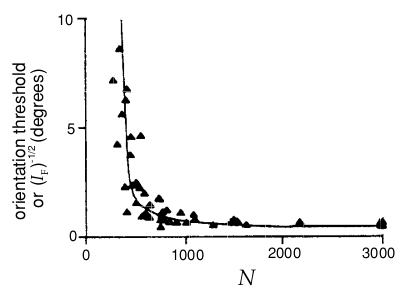
\includegraphics[scale = 0.6]{./png/3-12}
\end{center}
\end{exm}
















%%% Local Variables:
%%% mode: latex
%%% TeX-master: "../notesOnFluidMechanics"
%%% End:



\end{multicols}

%%% Local Variables:
%%% mode: latex
%%% TeX-master: "../notesOnFluidMechanics"
%%% End:


\chapter{Information Theory}
\label{cha:InformationTheory}

\begin{multicols}{2}
\setlength{\columnseprule}{0.2pt}  

\section{1.1}
\label{sec:1.1}

% \begin{defn}
%   The \emph{angular momentum},
%   also called \emph{moment of momentum} $\mathbf{L}$,
%   is the cross product of a moment arm $\mathbf{r}$ and
%   the linear momentum $m \mathbf{V}$ of a fluid particle,
%   i.e.,
%   \begin{equation}
%     \mathbf{L} = \mathbf{r}\times m\mathbf{V}.
%   \end{equation}
% \end{defn}
% \begin{center}
%   \includegraphics[scale=0.45]{./png/angularMomentumDefn}
% \end{center}

\begin{prin}[Conservation of angular momentum]
  \label{prin:angularMomentum}
  The rate of change of angular momentum of a system is equal to
  the net torque acting on the system,
  i.e.,
  \begin{equation}
    \frac{\dif \mathbf{L}}{\dif t} = \boldsymbol\tau,
  \end{equation}
  where $\boldsymbol\tau$ is the torque of all external forces on the system
  about any chosen axis,
  and $\dif \mathbf{L}/\dif t$ is the rate of change of
  angular momentum of the system about the same axis.
\end{prin}

% wo ai song jian jian
% wobuai bu xi zao de songjianjian

%%% Local Variables:
%%% mode: latex
%%% TeX-master: "../notesOnFluidMechanics"
%%% End:


\documentclass[letterpaper,oneside]{book}

\usepackage{geometry}
% make full use of A4 papers
\geometry{margin=1.5cm, vmargin={0pt,1cm}}
\setlength{\topmargin}{-1cm}
\setlength{\paperheight}{29.7cm}
\setlength{\textheight}{25.1cm}

% auto adjust the marginals
\usepackage{marginfix}

\usepackage{amsfonts}
\usepackage{amsmath}
\usepackage{amssymb}
\usepackage{amsthm}
\usepackage{CJKutf8}   % for Chinese characters
\usepackage{enumerate}
\usepackage{graphicx}  % for figures
\usepackage{layout}
\usepackage{multicol}  % multiple columns to reduce number of pages
\usepackage{mathrsfs}  
\usepackage{fancyhdr}
\usepackage{subfigure}
\usepackage{tcolorbox}
\usepackage{tikz-cd}
\usepackage{gensymb}
\usepackage{upgreek}
\usepackage{dsfont}

%------------------
% common commands %
%------------------
\newcommand{\dif}{\mathrm{d}}
\newcommand{\Dim}{\mathrm{D}}
\newcommand{\avg}[1]{\left\langle #1 \right\rangle}
\newcommand{\xibold}{\boldsymbol{\xi}}
\newcommand{\varphibold}{\boldsymbol{\varphi}}
\newcommand{\psibold}{\boldsymbol{\psi}}
\newcommand{\RE}{{\text{Re}}}

% this environment is for solutions of examples and exercises
\newenvironment{solution}%
{\noindent\textbf{Solution.}}%
{\qedhere}
% the following command is for disabling environments
%  so that their contents do not show up in the pdf.
\makeatletter
\newcommand{\voidenvironment}[1]{%
  \expandafter\providecommand\csname env@#1@save@env\endcsname{}%
  \expandafter\providecommand\csname env@#1@process\endcsname{}%
  \@ifundefined{#1}{}{\RenewEnviron{#1}{}}%
}
\makeatother

%----------------------------------------
% theorem and theorem-like environments %
%----------------------------------------
\numberwithin{equation}{chapter}
\theoremstyle{definition}

\newtheorem{thm}{Theorem}[chapter]
\newtheorem{alg}[thm]{Algorithm}
\newtheorem{asm}[thm]{Assumption}
\newtheorem{axm}[thm]{Axiom}
\newtheorem{coro}[thm]{Corollary}
\newtheorem{defn}[thm]{Definition}
\newtheorem{exm}[thm]{Example}
\newtheorem{exc}[thm]{Exercise}
\newtheorem{frm}[thm]{Formula}
\newtheorem{lem}[thm]{Lemma}
\newtheorem{ntn}{Notation}
\newtheorem{prop}[thm]{Proposition}
\newtheorem{rem}{Remark}[chapter]
\newtheorem{rul}[thm]{Rule}
\newtheorem{prin}[thm]{Principle}

\begin{document}
\pagestyle{empty}
\pagenumbering{roman}

%\tableofcontents
%\clearpage

\pagestyle{fancy}
\fancyhead{}
% \lhead{Yang Li}
% \chead{Notes on Fluid Mechanics}
% \rhead{2020}

%\setcounter{chapter}{-1}
\pagenumbering{arabic}
% \setcounter{page}{0}

% --------------------------------------------------------
% uncomment the following to remove these environments 
%  to generate handouts for students.
% --------------------------------------------------------
%\begingroup
%\voidenvironment{rem}%
%\voidenvironment{proof}%
%\voidenvironment{solution}%

% each chapter is factored into a separate file.

\chapter{Neual Encoding:Firing Rates and Spike Statics}
\label{cha:Firing Rates and Spike Statics}

\begin{multicols}{2} 
\setlength{\columnseprule}{0.2pt}  

\section{Spike Trains and Firing Rate}
\label{sec:firing rate}

\subsection{Firing Rate}

\begin{asm}
  Action potentials are typically treated as identical 
  stereotyped events in neural encoding
  studies ignoring in duration, amplitude, and shape. 
  We ignore the brief duration of an action potential (about 1 ms),
  an action potential sequence can be characterized simply by a list of the
  times when spikes occurred.
\end{asm} 

\begin{ntn}
  \emph{Spike train} is represented a list of the times $\{t_i\}_{i=1}^n$ when spikes occurred.
\end{ntn}

\begin{defn}
  \emph{Neural response function} $\rho (t)$ shows whether a spike is fired at time $t$,
   which can be represent as a sum of infinitesimally narrow, 
  idealized spikes in the form of Dirac $\delta$ functions
  \begin{equation}
    \label{equ:1.1}
    \rho(t)=\sum_{i=1}^n\delta(t-t_i),
  \end{equation}
  where $t_i$ with $i=1,2,\dots,n$, recorded in the trail, is the spike train
   %taken to 
   start at time $0$ and end at time $T$, so $0\leq t_i\leq T$ for all $i$.
\end{defn}

\begin{lem}
  $\delta$ function satisfies, for any well-behaved function $h(t)$
  \begin{equation}
    \label{equ:1.3}
    \int \delta(t-\tau)h(\tau)d\tau=h(t),
  \end{equation}
  \begin{proof}
  It follows from
  \begin{equation*}
    %\lim_{\epsilon\rightarrow 0}\int_{-\infty}^{+\infty} \delta(t-\tau)h(\tau)d\tau=
    \lim_{\epsilon\rightarrow 0}\int_{t - \epsilon}^{t + \epsilon} \delta(t-\tau)h(\tau)d\tau
    =h(t)\int_{t - \epsilon}^{t + \epsilon} \delta(t-\tau)d\tau=h(t)
  \end{equation*}
  \end{proof}
which provided that the limits of the integral surround the point $t$ (if they do not,
  the integral is $0$).
\end{lem}

\begin{thm}
  $\rho(t)$ is used to re-express sums over spikes as integrals over time. For any 
  well-behaved function $h(t)$, we can write
  \begin{equation}
    \label{equ:1.2}
    \sum_{i=1}^n h(t-t_i)=\int_{-\infty}^{\infty}h(\tau)\rho(t-\tau)d\tau,
  \end{equation}
  where the integral is over the duration of the trial.
  \begin{proof}
    The equation directly follows Equation \ref{equ:1.3}.
  \end{proof}
\end{thm}

\begin{defn}
  \emph{Spike-count rate $r$} is obtained by counting the number of action potentials that appear during a trial and
  dividing by the duration of the trial,
  \begin{equation}
    r=\frac{n}{T}=\frac{1}{T}\int_0^T\rho(\tau)d\tau.
  \end{equation}
  The second equality follows from the fact that $n=\int\rho(\tau)d\tau$ and indicates
that the spike-count rate is the time average of the neural response function over the 
duration of the trial.
\end{defn}

% \begin{rem}
%   A time-dependent fring rate can be defined by counting spikes over short time intervals, but this can no longer
% be computed from a single trial values. The solution to this problem is to average over multiple trials.
% \end{rem}

\begin{rem}
  The spike-count rate can be determined from a single trial, but at the expense of 
  losing all temporal resolution about variations in the neural response during the 
  course of the trial. A time-dependent firing rate can be defined by counting spikes 
  over short time intervals, but this can no longer
be computed from a single trial.
\end{rem}

\begin{exm}
  We can define the firing rate
at time $t$ during a trial by counting all the spikes that occurred between
times $t$ and $t + \Delta t$, for some small interval $\Delta t$, and dividing this count by
$\Delta t$. However, for small $\Delta t$, which allows for high temporal resolution, the
result of the spike count on any given trial is apt to be either $0$ or $1$, giving
only two possible firing-rate values.
\end{exm}

\begin{ntn}
  We use angle brackets, $\langle\ \rangle $, to denote averages over trials that use the same stimulus.
\end{ntn}

%\begin{exm}
 % The trial-averaged neural response function is denoted by $\langle \rho(t)\rangle $
%\end{exm}

\begin{defn}
  The \emph{time-dependent firing rate} r($t$) is the the average number of spikes (averaged over trials) appearing 
  during a
  short interval between times $t$ and $t+\Delta t$, divided by the duration of
   the interval,
   \begin{equation}
    \label{equ:1.5}
     r(t)=\frac{1}{\Delta t}\int_t^{t+\Delta t}\langle \rho(\tau)\rangle d\tau,
   \end{equation}
   where $\langle\rho(t)\rangle$ is the trial-averaged neural response function.
\end{defn}      

\begin{ntn}
  We use the notation r($t$) opposed to $r$ for the spike-count rate, and use the term 
  “firing rate” without any
modifiers, we mean r($t$).
\end{ntn}

\begin{rem}
  Formally, the limit $\Delta t\rightarrow 0$ should be taken on
the right side of Equation \ref{equ:1.5}, but, in extracting a time-dependent firing
rate from data, the value of $\Delta t$ must be large enough so there are sufficient
numbers of spikes within the interval defining r($t$) to obtain a reliable estimate of the 
average.
\end{rem}

\begin{prop}
  For sufficiently small $\Delta t$, $r(t)\Delta t$ 
  is the probability of a spike occurring during a short interval of duration $\Delta t$ around the time $t$.
  %which is called \emph{spiking probablity}.
  \begin{proof}
  For sufficiently small $\Delta t$, $r(t)\Delta t$ is the average number of spikes occurring
between times $t$ and $t + \Delta t$ over multiple trials. The average number of
spikes over a longer time interval is given by the integral of $r ( t )$ over that
interval. If $t$ is small, there will never be more than one spike within the
interval between $t$ and $t + \Delta t$ on any given trial. This means that $r(t)\Delta t$ is
also the fraction of trials on which a spike occurred between those times.
\end{proof}
\end{prop}



\begin{thm}
  For any function $h$, 
  we can
replace the trial-averaged neural response function with the firing rate r($t$)
within any well-behaved integral.
  \begin{equation}
    \label{equ:1.6}
    \int h(\tau)\langle \rho(t-\tau)\rangle d\tau = \int h(\tau)r(t-\tau)d\tau.
  \end{equation}
\end{thm}

\begin{rem}
  Equation \ref{equ:1.6} establishes an important relationship between the
average neural response function and the firing rate, the two are equivalent when used inside 
integrals. And provides another interpretation of
  r($t$) as the trial-averaged density of spikes along the time axis.
\end{rem}

\begin{defn}
  \emph{Average firing rate $\langle r \rangle $} is the spike-count firing rate to be averaged over trials.
  \begin{equation}
    \label{equ:1.7}
    \langle r\rangle =\frac{\langle n\rangle }{T}
    %=\frac{1}{T}\int_{0}^{T} \langle\rho(\tau) \rangle \,d\tau =\frac{1}{T}\int_{0}^{T}r(t)\,dt
  \end{equation}
   where $\langle n \rangle $ is the trial-averaged number of the spike in the trial, 
   $T$ is the time period of the trial.
\end{defn}

\begin{prop}
  \begin{equation*}
    \langle r\rangle=\frac{1}{T}\int_{0}^{T}r(t)\,dt
  \end{equation*}
  \begin{proof}
    \begin{equation*}
      \langle r\rangle =\frac{\langle n\rangle }{T}
    =\frac{1}{T}\int_{0}^{T} \langle\rho(\tau) \rangle \,d\tau =\frac{1}{T}\int_{0}^{T}r(t)\,dt
    \end{equation*}
    The first equality indicates that $\langle r\rangle $ is just the average 
   number of spikes per trial divided by the trial duration. The third equality follows from
the equivalence of the firing rate and the trial-averaged neural response
function within integrals Equation \ref{equ:1.6}. The average firing rate is equal to
both the time average of r($t$) and the trial average of the spike-count rate $r$. 
  \end{proof}
\end{prop}

\begin{rem}
  Whenever possible, we use the terms “firing rate”, “spike-count rate”
, and “average firing rate” for r($t)$, $r$, and $\langle  r\rangle  $, respectively. In particular, 
we distinguish the spike-count rate $r$
from the time-dependent firing rate r($t$) by
including the time argument in the latter expression (unless r($t)$ is independent of time).
\end{rem}

\subsection{Measuring Firing Rates}

\begin{ntn}
  The firing rate r($t$) cannot be determined exactly from the limited data
available from a finite number of trials. In addition, there is no unique
way to approximate r($t$).
  %In order to determine firing rate r($t$), we will introduce the concept of a linear filter and kernel.
  We illustrate the methods of measuring firing rate by extracting
  firing rates from a single trial, but more accurate results could be obtained
  by averaging over multiple trials.
  \begin{exm}
    We shows $3$s of the response of a neuron in the inferotemporal cortex 
  recorded while a monkey watched a video. Neurons
  in the region of cortex where this recording was made are selective for
  complex visual images, including faces.
  \end{exm}
\end{ntn}
\begin{center}
  \label{fig:1.4A}
    \includegraphics[scale=0.048]{./png/fig:1.4A.jpg}
  \end{center}

\begin{alg}
  A simple algorithm of extracting an estimate of the firing rate from a spike train is to divide time into
discrete bins of duration $\Delta t$, count the number of spikes within each bin,
and divide by $\Delta t$.
\end{alg}

\begin{exm}
  This figure shows the approximate firing rate computed
using this procedure with a bin size of 100 ms. Note that with this procedure, the quantity being computed is 
really the spike-count firing rate over the duration of the bin, and that the firing rate 
r($t$) within a 
given bin is approximated by this spike-count rate. The binning and counting procedure 
illustrated in this figure 
generates an estimate of the firing rate that is a piecewise constant function of time, 
resembling a histogram.
\end{exm}

\begin{center}
  \label{fig:1.4B}
  \includegraphics[scale=0.053]{./png/fig:1.4B.jpg}
\end{center}

\begin{lem}
   Because spike counts can take only integer values, the rates computed by this method will 
   always 
  be integer multiples of $1 / \Delta t$, and thus they take discrete values. Decreasing 
  the value of $\Delta t$
increases temporal resolution by providing an estimate of the firing rate at
more finely spaced intervals of time, but at the expense of decreasing the
resolution for distinguishing different rates.
\end{lem}

\begin{alg}
  One algorithm to avoid quantized
firing rates is to vary the bin size so that a fixed number of spikes appears
in each bin. The firing rate is then approximated as that fixed number of
spikes divided by the variable bin width.
\end{alg}

\begin{rem}
  Counting spikes in preassigned bins produces a firing-rate estimate that
depends not only on the size of the time bins but also on their placement.
\end{rem}

\begin{alg}
To avoid the arbitrariness in the placement of bins, the algorithm is taking
a single bin or window of duration $\Delta t$ and slide it along the spike train,
counting the number of spikes within the window at each location which have a better 
temporal resolution.
\end{alg}

\begin{exm}
  \label{fig:1.4C}
  The jagged curve in  the figure below shows the result of sliding a $100$ ms wide
window along the spike train.  The firing rate approximated in 
this way
can be expressed as the sum of a window function over the times $t_i$ for
$i = 1 , 2 ,\dots, n$ when the $n$ spikes in a particular sequence occurred,
\begin{equation}
  \label{equ:1.8}
  r_{\text{approx}}(t)=\sum_{i = 1}^{n}\omega(t-t_i), 
\end{equation}
where the window function is

\begin{equation}
  \label{equ:1.9}
  \omega(t)=\left\{
    \begin{aligned}
      1/\Delta t \quad &\text{if} -\Delta t/2\leq t\leq \Delta t/2\\
      0 \quad & \text{otherwise}.
    \end{aligned}
  \right.
\end{equation}
The jagged appearance of the curve is caused 
by the discontinuous shape of the window function used.
\end{exm}

\begin{center}
  \includegraphics[scale=0.054]{./png/fig:1.4C.jpg}
\end{center}

\begin{prop}
  The sum in Equation\ref{equ:1.8} can also be written as the integral of the window
function times the neural response function
\begin{equation}
  \label{equ:1.10}
  r_{\text{approx}}(t)=\int_{-\infty}^{\infty}\omega(\tau)\rho(t-\tau)d\tau.
\end{equation}
\begin{proof}
  The proof directly follows Equation\ref{equ:1.2}.
\end{proof}
\end{prop}

\begin{defn}
  The integral in Equation \ref{equ:1.10} is called a \emph{linear filter}, and the window 
  function $\omega$, also called the \emph{filter kernel}, specifies how the neural 
  response function evaluated at time $t-\tau$ contributes to the firing rate approximated 
  at time $t$.
\end{defn}

\begin{exm}
  \label{fig:1.4D}
  Instead of the rectangular window function used in figure in example \ref{fig:1.4C}, 
  figure in example \ref{fig:1.4D} use a 
  continuous window function like the Gaussian
  \begin{equation}
    \label{equ:1.11}
    w(\tau)=\frac{1}{\sqrt{2\pi}}\sigma_{\omega}\text{exp}\left(-\frac{\tau^2}{2\sigma_{\omega}^2} \right),  
  \end{equation}
   which is used in Equation \ref{equ:1.8} generates 
a firing-rate estimate that is a smooth function of time.
In this case, $\sigma_{\omega}$  controls the temporal resolution of the resulting rate, 
playing a role analogous to $\Delta t$.
\end{exm}

\begin{center}
  \includegraphics[scale=0.245]{./png/fig:1.4D.png}
\end{center}

\begin{prin}
  A postsynaptic neuron monitoring the spike train of a presynaptic cell has
access only to spikes that have previously occurred.
\end{prin}

\begin{defn}
  A window function or kernel is called \emph{causal} when an approximation
of the firing rate at time $t$ that depends only on spikes fired before $t$ can
be calculated using a window function that vanishes when its argument is negative.

\end{defn}

\begin{defn}
  The \emph{half-wave rectification} $[z]_+$ for any quantity $z$ stands for,
\begin{equation}
  \label{equ:1.13}
  [z]_+ =\left\{
    \begin{aligned}
      z \quad &\text{if} \quad z\geqslant 0\\
      0 \quad & \text{otherwise}.
    \end{aligned}
  \right.
\end{equation}
\end{defn}

\begin{exm}
  \label{fig:1.4E}
  One commonly used window function is the $\alpha$ function
  \begin{equation}
    w(\tau)=[\alpha^2 \tau \text{exp}(-\alpha\tau) ]_+ 
  \end{equation}
  where $1/\alpha$ determines the temporal resolution of the resulting firing-rate
 estimate. The figure below shows the firing rate approximated by such a causal scheme.
\end{exm}

\begin{center}
  \includegraphics[scale=0.72]{./png/fig:1.4E.png}
\end{center}

\begin{rem}
  Note that the rate computed in example \ref{fig:1.4E} tends to peak later than the 
  rate computed in example \ref{fig:1.4D} using a temporally symmetric window function.%%这个地方需要解释一下吗?
\end{rem}

\subsection{Tuning Curve}

\begin{rem}
  Neuronal responses typically depend on many different properties of a
stimulus. In this chapter, we characterize responses of neurons as functions of 
just one of the stimulus attributes to which they may be sensitive. The value of this 
single attribute is denoted by \emph{s}. In chapter ??, we consider
more complete stimulus characterizations.
\end{rem}

\begin{defn}
  The \emph{neural response tuning curve} is the average firing rate written 
  as a function of $s$, $\langle r\rangle =f(s)$. The functional form of a tuning 
  curve depends on the parameter $s$ used to describe the stimulus. 
  %The precise choice of parameters used as arguments of tuning curve functions is partially a matter of convention.
\end{defn}

\begin{rem}
  A simple way of characterizing the response of a neuron is to count the
number of action potentials fired during the presentation of a stimulus.
This approach is most appropriate if the parameter $s$ characterizing the
stimulus is held constant over the trial. If we average the number of action potentials 
fired over (in theory, an infinite number of) trials and divide by the trial duration, 
we obtain the average firing rate, $ \langle r\rangle$, defined in Equation \ref{equ:1.7}.
\end{rem}

\begin{ntn}
  Because tuning curves correspond to firing rates, they are measured in units of spikes 
  per second or Hz.
\end{ntn}

\begin{exm}
  \label{fig:1.5}
   We show extracellular recordings of a neuron in the primary visual cortex (V1) of 
a monkey. While these recordings were being made, a
bar of light was moved at different angles across the region of the visual
field where the cell responded to light. This region is called the receptive 
field of the neuron. Note that the number of action potentials fired
depends on the angle of orientation of the bar.

The dots in the figure B of example \ref{fig:1.5} indicate the average firing rate depends on the degrees of the orientation angle of the light bar stimulus.

The data have been fitted by a response tuning curve of the form of \emph{Gaussian tuning curve}
\begin{equation}
  \label{equ:1.14}
  f(s)=r_{\text{max}}\text{exp}\left(-\frac{1}{2}\left(\frac{s-s_{\text{max}}}{\sigma_f}\right)^2\right),
\end{equation}

The curve  in figure B is a fit using
the Equation \ref{equ:1.14} with parameters $r_{\text{max}} = 52 . 14 $Hz, $s_{\text{max}}= 0 ^\circ$,
 and $\sigma_f= 14 . 73 ^\circ $,
where $s$ is the orientation angle of the light bar, $s_{\text{max}}$ is the orientation angle
evoking the maximum average response rate $r_{\text{max}}$ (with $s-s_{\text{max}} $ taken 
to lie in the range between $- 90^\circ $ and $+90^\circ$  ), and $\sigma_f$ determines the 
width of the tuning curve. The neuron responds most vigorously when a stimulus
having $s=s_{\text{max}} $ is presented, so we call $s_{\text{max}}$ the preferred orientation angle
of the neuron.

\begin{center}
  \includegraphics[scale=0.38]{./png/fig:1.5.png}
\end{center}
\end{exm}

\begin{rem}
  Tuning curves can also be measured for neurons in motor areas, in which
case the average firing rate is expressed as a function of one or more parameters describing 
a motor action.
\end{rem}

\begin{exm}
  \label{fig:1.6}
  We show an example of extracellular recordings from a neuron in primary motor cortex 
  in a monkey
  that has been trained to reach in different directions. The stacked traces for
  each direction are rasters showing the results of five different trials. The
  horizontal axis in these traces represents time, and each mark indicates
  an action potential. The firing pattern of the cell, in particular the rate at
  which spikes are generated, is correlated with the direction of arm movement.% and thus 
  encodes information about this aspect of the motor action.

  The dots in figure B of example \ref{fig:1.6} indicate the average firing rate depends 
  on the degrees of the direction of the arm movement.
  Here the data points have
  been fitted by a tuning curve in the form of a \emph{cosine tuning curve} to be half-wave 
  rectified.
\begin{equation}
    \label{equ:1.16}
    f(s)=[r_0+\left(r_{\text{max}}-r_0\right)\cos\left(s-s_{\text{max}}\right)]_+.
  \end{equation}

  where $s$ is the reaching angle of the arm, $s_{\text{max}}=161.25^\circ$ is the reaching 
  angle associated with the maximum response $r_{\text{max}}$, and $r_0=32.34$ Hz is an 
  offset or background
  firing rate that shifts the tuning curve up from the zero axis. 
  \begin{center}
    \includegraphics[scale=0.34]{./png/fig:1.6.png}
  \end{center}
\end{exm}

\begin{exm}
  \label{fig:1.7}
  The mode of retinal disparity. The gray lines with arrows show the
location on each retina of an object located nearer than the fixation point F. The
image from the fixation point falls at the fovea in each eye, the small pit where
the black lines meet the retina. The image from a nearer object falls to the left of
the fovea in the left eye and to the right of the fovea in the right eye. For objects
farther away than the fixation point, this would be reversed. The disparity angle $s$
is indicated in the figure.

The dots in figure B of example \ref{fig:1.7} indicate average firing rate of a V1 neuron depends on
retinal disparity and illustrates another important type of tuning curve.

Here the data points have been fitted with a tuning curve called
a logistic or sigmoidal function,
\begin{equation}
  \label{equ:1.17}
  f(s)=\frac{r_{\text{max}}}{1+\exp\left(\left(s_{1/2}-s\right)/\Delta_s\right)}.
\end{equation}
In this case, $s$ is the retinal disparity, the parameter $s_{1/2}$ is the disparity
that produces a firing rate half as big as the maximum value $r_{\text{max}}$ , and $\Delta_s$
controls how quickly the firing rate increases as a function of $s$. If $\Delta_s$ is
negative, the firing rate is a monotonically decreasing function of $s$ rather
than a monotonically increasing function.
\begin{center}
  \includegraphics[scale=0.39]{./png/fig:1.7.png}
\end{center}
\end{exm}

\subsection{Spike-Count Variability}
\begin{rem}
  Tuning curves allow us to predict the average firing rate, but they do not
describe how the spike-count firing rate $r$ varies about its mean value $\langle r\rangle=f(s) $ 
from trial to trial. While the map from stimulus to average
response may be described deterministically, it is likely that single-trial
responses such as spike-count rates can be modeled only in a probabilistic manner.
Generally, $r$ values can be generated from a probability
distribution with mean $f(s)$.
\end{rem}

\begin{defn}
  The trial-to-trial deviation of $r$ from $f ( s )$ is
considered to be noise, and such models are often called \emph{noise models}.
\end{defn}
\begin{defn}
  The standard deviation for the noise distribution either can be independent of 
  $f ( s )$, in which case is called \emph{additive noise}, or it can
depend on $f ( s )$. \emph{Multiplicative noise} corresponds to having the standard
deviation proportional to $f ( s )$.
\end{defn}



%\bibliography{bib/numericalApprox}
%\bibliographystyle{abbrv}
%\bibliographystyle{abbrvnat}
%\setcitestyle{authoryear,open={[},close={]}}
\end{multicols}
\end{document}


%%% Local Variables: 
%%% mode: latex
%%% TeX-master: t
%%% End: 


\section{Population Decoding}
\label{sec:Population Decoding}

\begin{rem}
  The use of large numbers of neurons to represent information is a basic
operating principles of many nervous systems. \emph{Population coding} has a
number of advantages, including reduction of uncertainty due to neuronal
variability and the ability to represent a number of different
stimulus attributes simultaneously. In the previous section, we
discussed discrimination between stimuli on the basis of the response of
a single neuron. The responses of a population of neurons can also be
used for discrimination, with the only essential difference being that terms
such as $p[r|s]$ are replaced by $p[\mathbf{r}|s]$, the conditional
probability density of the population response $\mathbf{r}$. ROC
analysis, likelihood ratio tests, and the Neyman-Pearson lemma continue to apply in exactly the same way.
\end{rem}

\begin{rem}
  \emph{Discrimination} is a special case of decoding in which only a
  few different stimulus values are considered. A more general problem
  is the extraction of a continuous stimulus parameter from one or
  more neuronal responses. In this section, we study how the value of a continuous parameter associated with a static stimulus can be decoded from the spike-count firing
rates of a population of neurons.
\end{rem}

\subsection{Encoding and Decoding Direction}
\begin{exm}
  The cercal system of the cricket, which senses the direction of incoming air
currents is an interesting example of population coding involving a
four interneurons. The figure shows average firing-rate tuning curves
for the four relevant interneurons as a function of wind
direction, which are well approximated by halfwave rectifed cosine
function. The preferred directions of the neurons are located $90^{\circ}$ from each other, and $r_{\max}$
values are typically around 40 Hz.
\end{exm}

\begin{center}
  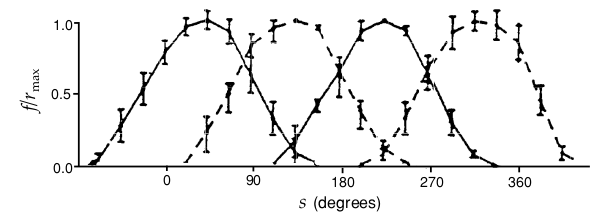
\includegraphics[scale = 0.4]{./png/3-4}
\end{center}

\begin{prop}
  \label{prop:single neuron cosine function}
  Neuron $a$ (where $a=1,2,3,4$) responds
with a maximum average firing rate when the angle of the wind direction
is $s_{a}$, the preferred-direction angle for that neuron. The tuning curve for
interneuron a in response to wind direction $s$, $\left\langle r_{a}
\right\rangle=f_a(s)$, normalized to its maximum, can be written as
\begin{equation}
  \label{eq:3.20}
  \Big( \frac{f(s)}{r_{\max}} \Big)_{a}=[(\cos(s-s_a))]_+,
\end{equation}
where the half-wave rectifcation eliminates negative firing rates. Here
$r_{\max}$, which may be different for each neuron, is a constant equal to the
maximum average firing rate.
\end{prop}

\begin{prop}
 For  the cercal system of the cricket, Equation \ref{eq:3.20} can be written as
  \begin{equation}
  \label{eq:3.21}
 \Big( \frac{f(s)}{r_{\max}} \Big)_{a}=[\vec{v}\cdot\vec{c}_a].
\end{equation}
where spatial vector $\vec{v}$ pointing parallel to the wind velocity in place of the angle
$s$ and having unit length $\big| \vec{v} \big|=1$ and a vector
  $\vec{c}_{a}$  of unit length is the preferred wind direction  pointing in the
  direction specified by the angle $s_{a}$ for each interneuron.

\begin{proof}
In this case, we can use the vector dot product to write
$\cos(s-s_a)=\vec{v}\cdot\vec{c}_a$. In terms of these
vectors, the average firing rate is proportional to a half-wave
rectified projection of the wind direction vector onto the
preferred direction axis of the neuron. And combined with the above
proposition \ref{prop:single neuron cosine function}, we give the answer.
\end{proof}

\end{prop}

\begin{rem}
  Decoding the cercal system is particularly easy because of the close relationship between the representation of wind direction it provides and a
two-dimensional Cartesian coordinate system. The preferred directions
of the four interneurons, like the $x$ and $y$ axes of a Cartesian coordinate
system, lie along two perpendicular directions. Four neurons
are required, rather than two, because firing rates cannot represent negative projections.
\end{rem}

\begin{prop}
  If $r_{a}$ is the spike-count fring rate of neuron $a$, an estimate of
  the wind direction on any given trial can be obtained from the
  direction of the vector
  \begin{equation}
    \label{eq:3.22}
    \vec{v}_{\rm{pop}}=\sum\limits_{a=1}^4\left( \frac{r}{r_{\max}} \right)_a\vec{c}_a.
  \end{equation}
  This vector is known as the \emph{population vector}, and the associated decoding
  method is called the \emph{vector method}. In fact, this encoding is
  the one that requires the least number of neurons to encode
  two-dimensional directions.
\end{prop}

\begin{exm}
In figure A, preferred directions of four cercal interneurons in relation to the
cricket’s body. The firing rate of each neuron for a fixed wind speed is proportional to the projection of the wind velocity vector $\vec{v}$ onto the preferred-direction
axis of the neuron. The projection directions
$\vec{c}_{1}$, $\vec{c}_{2}$, $\vec{c}_{3}$, and $\vec{c}_{4}$ for the four neurons
are separated by  $90^{\circ}$, and they collectively form a Cartesian coordinate system.
In figure B, the root-mean-square error in the wind direction determined by vector decoding of the firing rates of four cercal interneurons. These results were obtained
through simulation by randomly generating interneuron responses to a variety of
wind directions, with the average values and trial-to-trial variability of the firing
rates matched to the experimental data. The generated rates were then decoded
using Equation \ref{eq:3.22} and compared to the wind direction used
to generate them.
   \begin{center}
    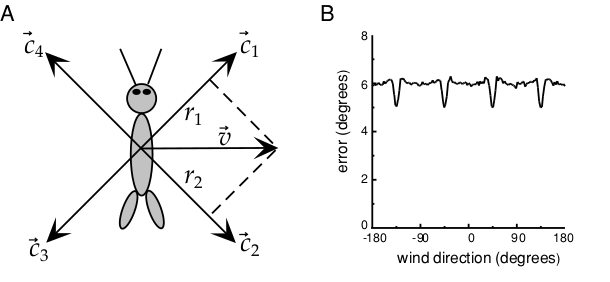
\includegraphics[scale = 0.4]{./png/3-5}
    \label{fig:3.5AB}
  \end{center}
  \end{exm}

\begin{exm}
  As discussed in chapter \ref{cha:Neural Encoding I}, tuning curves of certain neurons in the primary
motor cortex (M1) of the monkey can be described by cosine functions of
arm movement direction. Thus, a vector decomposition similar to that
of the cercal system appears to take place in M1. Many M1 neurons have
nonzero offset rates, $r_{0}$. When an arm movement is made in the direction represented by a vector of unit length, $\vec{v}$, the average fring rates for such a M1
neuron, labeled by an index $a$, can be written as
\begin{equation}
  \label{eq:3.23}
  \left( \frac{\left\langle r \right\rangle-r_{0} }{r_{\max}}\right)_{a}=\left( \frac{f(s)-r_{0}}{r_{\max}} \right)_{a}=\vec{v}\cdot\vec{c}_a,
\end{equation}
where $\vec{c}_a$ is the preferred-direction vector that defines the
selectivity of the neuron. Unlike the cercal interneurons, M1 neurons
do not have orthogonal preferred directions that form a Cartesian
coordinate system. Instead, the preferred directions of the neurons appear to point in all directions with
roughly equal probability.
\end{exm}

\begin{prop}
  If the preferred directions point uniformly in all directions and
  the number of neurons $N$ is suffciently large, the population vector
  \begin{equation}
      \label{eq:3.24}
    \vec{v}_{\rm{pop}}=\sum\limits_{a=1}^N \left( \frac{r-r_{0}}{r_{\max}} \right)_a\vec{c}_a,
  \end{equation}
will, on average, point in a direction parallel to the arm movement direction vector $\vec{c}$. If we average Equation \ref{eq:3.24} over
trials and use Equation \ref{eq:3.23}, we find
\begin{equation}
  \label{eq:3.25}
  \left\langle  \vec{v}_{\rm{pop}} \right\rangle=\sum_{a=1}^N{(\vec{v}\cdot\vec{c}_a)\vec{c}_a},
\end{equation}
 where $\vec{v}_{\rm{pop}}$ is approximately parallel
to $\vec{v}$ if a large enough number of neurons is included in the sum, and
if their preferred-direction vectors point randomly in all directions with
equal probability.
\end{prop}

\subsection{Optimal Decoding Methods}

\begin{rem}
  The vector method is a simple decoding method that can perform quite
well in certain cases, but it is neither a general nor an optimal way
to reconstruct a stimulus from the fring rates of a population of
neurons. In
this section, we dicuss two methods, that are Bayesian inference and MAP
inference, which are considered optimal by some measure.
\end{rem}

\begin{rem}
  \emph{Bayesian} and \emph{MAP} estimates use the conditional
  probability that a stimulus parameter takes a value between $s$ and
  $s+\nabla s$, given that the set of $N$ encoding neurons fired at
  rates given by $\mathbf{r}$. The probability density needed for a
  continuous stimulus parameter, $p[s|\mathbf{r}]$, can be obtained from
  the encoding probability density $p[\mathbf{r}|s]$ by the continuous version of Bayes
theorem,
\begin{equation}
  \label{eq:3.26}
  p[s|\mathbf{r}]=\frac{p[\mathbf{r}|s]p[s]}{p[\mathbf{r}]}.
\end{equation}
A disadvantage of these methods is that extracting $p[s|\mathbf{r}]$ from experimental data can be diffcult.
\end{rem}

\begin{defn}
  Below are the two optimal ways to reconstruct a stimulus from the
  fring rates of a population of neurons:
  \begin{enumerate}[(i)]
  \item The \emph{Bayesian inference} involves finding the minimum of a loss
  function $L(s,s_{\rm{bayes}})$ that quantifyes the cost of reporting
  the estimate $s_{\rm{bayes}}$ when the correct answer is $s$.
  \item  The \emph{MAP inference} chooses the stimulus value, $s_{\rm{MAP}}$,
  that maximizes the conditional probability density of the stimulus,
  $p[s_{\rm{MAP}}|\mathbf{r}]$ and \emph{ML inference} chooses
  $s_{\rm{ML}}$ to maximize the likelihood function,
  $p[\mathbf{r}|s_{\rm{ML}}]$, which generally produce estimates
  that are as accurate, in terms of the variance of the estimate, as
  any that can be achieved by a wide class of estimation methods
  (so-called unbiased estimates).
  \end{enumerate}
\end{defn}

\begin{rem}
  The value of $s_{\rm{bayes}}$ is chosen to minimize the expected
loss averaged over all stimuli for a given set of rates, that is, to minimize
the function $\int L(s,s_{\rm{bayes}})p[s|\mathbf{r}]ds$.
\end{rem}

\begin{exm}
  If the loss function is the squared difference between the estimate
  and the true value, $ L(s,s_{\rm{bayes}})=(s-s_{\rm{bayes}})^{2}$, the
  estimate that minimizes the expected loss is the mean
  \begin{equation}
    \label{eq:3.27}
    s_{\rm{bayes}}=\int p[s|\mathbf{r}]ds.
  \end{equation}
\end{exm}

\begin{exm}
 If the loss function is the absolute value of the
 difference, $L(s,s_{\rm{bayes}})=\big|s-s_{\rm{bayes}} \big|$, then
 $s_{\rm{bayes}}$ is the median rather than the mean of the
 distribution $p[s|\mathbf{r}]$.
\end{exm}


\begin{rem}
  The MAP approach is thus to choose as the estimate $s_{\rm{MAP}}$ the most
  likely stimulus value for a given set of rates. If the prior or
  stimulus probability density $p[s]$ is independent of $s$, then
  $p[s|\mathbf{r}]$ and $p[\mathbf{r}|s]$ have the same dependence on
  $s$, because the factor $p[s]/p[\mathbf{r}]$ in Equation \ref{eq:3.26} is independent of $s$. In this case, the MAP algorithm is equivalent to  maximum likelihood (ML) inference.
\end{rem}

\begin{exm}
  The root-mean-squared difference between
the true and estimated wind directions for the cercal system, using ML
and Bayesian methods is shown as follows. The Bayesian estimate in figure is based on the squared-difference loss function. Both
estimates use a constant stimulus probability density $p[s]$, so the ML and
MAP estimates are identical. The Bayesian result has a slightly
smaller average error across all angles. The dips in the error curves in figure
appear at angles where one tuning curve peaks and two others rise from
threshold. These dips are due to the two
neurons responding near threshold, not to the maximally responding neu-
ron. They occur because neurons are most sensitive at points where their
tuning curves have maximum slopes, which in this case is near threshold.
\begin{center}
  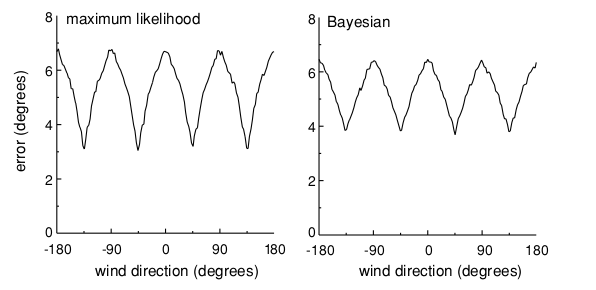
\includegraphics[scale = 0.4]{./png/3-7}
\end{center}
\end{exm}


\begin{exm}
  \label{exm:Gaussian tuning curves}
  Up to now, we have considered the decoding of a direction angle. We now
turn to the more general case of decoding an arbitrary continuous stimulus
parameter. An instructive example is provided by an array of $n$ neurons
with preferred stimulus values distributed uniformly across the full range
of possible stimulus values. An example of such an array for Gaussian
tuning curves,
\begin{equation}
  \label{eq:3.28}
  f_a(s)=r_{\rm{max}}\exp\left(-\frac{1}{2}\left(
      \frac{s-s_{a}}{\sigma_{a}} \right)^{2}\right).
\end{equation}
In this example, each neuron has a tuning curve
with a different preferred value $s_{a}$ and potentially a different
width $\sigma_{a}$. If the tuning curves are evenly and densely distributed across the range of $s$ values, the
sum of all tuning curves
$\sum f_a(s)$ is approximately independent of $s$. The roughly flat line is proportional to this sum.
\begin{center}
  \label{fig:3-8}
  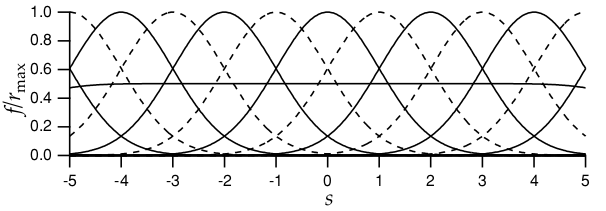
\includegraphics[scale = 0.4]{./png/3-8}
\end{center}
\end{exm}

\begin{rem}
  To implement the Bayesian, MAP, or ML approach, we need to
know the conditional firing-rate probability density $p[\mathbf{r}|s]$ that describes
this variability.
\end{rem}

\begin{prop}
  \label{prop:conditional firing-rate probability density}
  We assume that the firing rate $r_{a}$ of neuron $a$ is determined
by counting $n_{a}$ spikes over a trial of duration $T$ (so that $r_{a} = n_{a}/T$), and
that the variability can be described by the homogeneous Poisson model
discussed in chapter \ref{cha:Neural Encoding I}. In this case, the probability of stimulus s evoking
$n_{a}=r_{a}T$ spikes, when the average firing rate is $\left\langle
  r_{a} \right\rangle=f_a(s)$, is given by
\begin{equation}
  \label{eq:3.29}
  P[r_a|s]=\frac{(f_a(s)T)^{r_aT}}{(r_aT)!}\exp(-f_{a}(s)T).
\end{equation}
If we assume that each neuron fires independently, the firing-rate
probability for the population is the product of the individual
probabilities,
\begin{equation}
  \label{eq:3.30}
   P[\mathbf{r}|s]=\prod\limits_{a=1}\limits^{N}{\frac{(f_a(s)T)^{r_{a}T}} {(r_aT)!}\exp(-f_{a}(s)T)}.
\end{equation}
\end{prop}

\begin{exm}
  The filled circles in figure show a set of randomly generated firing rates
for the array of Gaussian tuning curves for $s=0$ shown above. This figure
also illustrates a useful way of visualizing population responses: plotting
the responses as a function of the preferred stimulus values. The dashed
curve is the tuning curve for the neuron with $s_{a}=0$. Because
the tuning curves are functions of $\left| s-s_{a} \right|$, the values of the dashed curve at
$s_{a}=-5,-4,\dots,5$ are the mean activities of the cells with preferred values
at those locations for a stimulus at $s=0$.
\begin{center}
    \label{fig:3-9}
  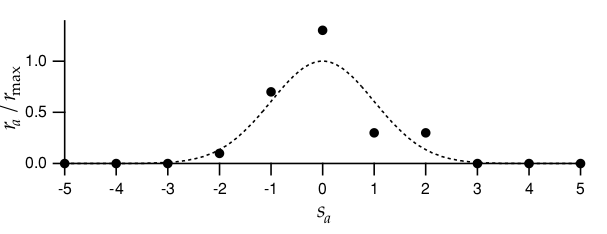
\includegraphics[scale = 0.4]{./png/3-9}
\end{center}
\end{exm}

\begin{prop}
  The ML estimated stimulus, $s_{ML}$, is the stimulus that maximizes $P[\mathbf{r}|s]$. We
find that $s_{\rm{ML}}$ is determined by
\begin{equation*}
  T\sum\limits_{a=1}\limits^{N}{r_{a}\frac{f_{a}'(s_{ML})}{f_{a}(s_{ML})}}=0,
\end{equation*}
where the prime denotes a derivative.
\begin{proof}
 To apply the ML estimation algorithm, we only need to consider the terms
in $P[\mathbf{r}|s]$ that depend on $s$. Because Equation
\ref{eq:3.30} involves a product, it is convenient to take its logarithm and write
\begin{equation}
  \label{eq:3.31}
  \ln P[\mathbf{r}|s]=T\sum\limits_{a=1}\limits^{N}{r_{a}\ln \left( f_a(s) \right)}+\dots,
\end{equation}
where the ellipsis represents terms that are independent
or approximately independent of $s$, including, as discussed above,
$\sum{f_a(s)}$.
 Setting the derivative to $0$, we give the answer.
 \end{proof}
\end{prop}

\begin{exm}
  If the tuning curves are the Gaussians of Equation \ref{eq:3.28},
  this equation can be solved explicitly using the result
  $f_{a}'(s)/f_a(s)=(s_{a}-s)/\sigma_{a}^{2}$,
    \begin{equation}
      \label{eq:3.33}
      s_{\rm{ML}}=\frac{\sum{r_as_a/\sigma_{a}^{2}}}{\sum{r_a/\sigma_{a}^{2}}}.
    \end{equation}
    If all the tuning curves have the same width, this reduces to
    \begin{equation}
      \label{eq:3.34}
      s_{\rm{ML}}=\frac{\sum{r_as_a}}{\sum{r_a}},
  \end{equation}
  which is a simple estimation formula with an intuitive interpretation as
the firing-rate weighted average of the preferred values of the encoding
neurons.
\end{exm}

\begin{rem}
  Although the stimuli obtained by maximum likelihood estimation are
  the weighted average of the best responses. This result looks very
  good, but under the influence of noise, this method may reduce the
  accuracy. The MAP algorithm allows us to include prior knowledge $p[s]$
about the distribution of stimulus values in the decoding estimate. When using
  MAP, The objective function will have one more term $\log(p[s])$
  and the maximum value can still be obtained by derivation. If the
  $p[s]$ is constant, the MAP and ML estimates are
  identical.

   Inaddition, if many neurons are observed, or if a small
  number of neurons is observed over a long trial period, even a
  nonconstant stimulus distribution has little effect and $s_{\rm{MAP}}\approx s_{\rm{ML}}$.
\end{rem}

\begin{prop}
  The MAP estimate is computed from the distribution $p[s|\mathbf{r}]$ determined by
Bayes theorem. In terms of the logarithms of the probabilities, $\ln
p[s|\mathbf{r}]=\ln p[\mathbf{r}|s]+\ln p[s]-\ln P[r]$. The last
term in this expression is independent of $s$ and can be absorbed into the ignored $s$-independent terms, so we can
write, as in Equation \ref{eq:3.31},
\begin{equation}
  \label{eq:3.35}
 \ln p[s|\mathbf{r}]=T\sum\limits_{a=1}\limits^{N}{r_{a}\ln \left(
     f_a(s) \right)+\ln p[s]+\dots}.
 \end{equation}
 Maximizing this determines the MAP estimate,
 \begin{equation}
   \label{eq:3.36}
    T\sum\limits_{a=1}\limits^{N}{\frac{r_{a}f_{a}'(s_{\rm{MAP}})}{f_{a}(s_{MAP})}}+\frac{p'[s_{\rm{MAP}}]}{p[s_{\rm{MAP}}]}=0.
 \end{equation}
\end{prop}

\begin{exm}
  If the stimulus or prior distribution is itself Gaussian with mean
  $s_{\rm{prior}}$  and
variance  $\sigma_{\rm{prior}}$ , and we use the Gaussian array of tuning curves,
Equation \ref{eq:3.36} yields
\begin{equation}
  \label{eq:3.37}
s_{\rm{MAP}}=\frac{T\sum{r_as_a}/\sigma_a^{2}+s_{\rm{prior}}/\sigma_{{\rm{prior}}}^{2}}{T\sum{r_a/\sigma_a^{2}}+1/\sigma_{{\rm{prior}}}^{2}}.
\end{equation}
\end{exm}

\begin{exm}
  The figure compares the conditional stimulus probability densities $p[s|\mathbf{r}]$
for a constant stimulus distribution (solid curve) and for a Gaussian stimulus distribution with $s_{\rm{prior}}=-2$ and $\sigma_{{\rm{prior}}}=1$, using the firing rates given
by the filled circles in last figure. If the stimulus distribution is constant,
$p[s|\mathbf{r}]$ peaks near the true stimulus value of $0$. The effect of a noncon-
stant stimulus distribution is to shift the curve toward the value $-2$, where
the stimulus probability density has its maximum, and to decrease its
width by a small amount. The estimate is shifted to the left because the
prior distribution suggests that the stimulus is more likely to take
negative values than positive ones, independent of the evoked
response. The decreased width is due to the added information that the prior distribution provides.

\begin{center}
    \label{fig:3-10}
  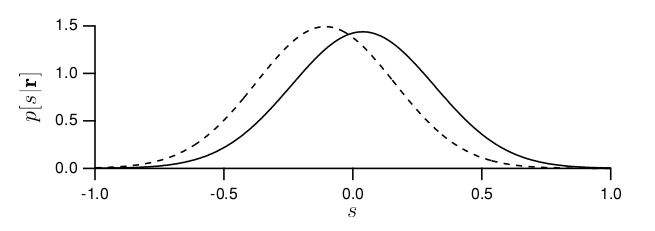
\includegraphics[scale = 0.4]{./png/3-10}
\end{center}
\end{exm}


\begin{defn}
  \label{defn:bias}
  The accuracy with which an estimate $s_{\rm{est}}$ describes a
  stimulus $s$ can be characterized by two important quantities, its
  bias $b_{\rm{est}}(s)$ and its variance
$\sigma_{\rm{est}}^{2}(s)$. The bias is the difference between the
average of $s_{\rm{est}}$ across trials that use the stimulus $s$ and the true
value of the stimulus (i.e., $s$),
\begin{equation}
  \label{eq:3.38}
  b_{\rm{est}}(s)=\left\langle s_{\rm{est}} \right\rangle-s.
\end{equation}
\end{defn}

\begin{defn}
  An estimate is termed unbiased if $b_{\rm{est}}(s)=0$ for all stimulus values.
\end{defn}

\begin{defn}
  The variance of the estimator, which quantifies how much the estimate
  varies about its mean value, is defined as
  \begin{equation}
    \label{eq:3.39}
    \sigma_{\rm{est}}^{2}(s)=\left\langle (s_{\rm{est}} -\left\langle s_{\rm{est}}  \right\rangle)^{2} \right\rangle.
  \end{equation}
\end{defn}

\begin{prop}
  The bias and variance can be used to compute the trial-average
  squared estimation error, $\left\langle (s_{\rm{est}} -s)^{2}\right\rangle$. This is a measure of the spread of the estimated values about the true value of the stimulus. Considering Definition \ref{defn:bias}, we can write the squared estimation error as
    \begin{equation}
      \label{eq:3.40}
      \left\langle (s_{\rm{est}} -s)^{2} \right\rangle=\left\langle (s_{\rm{est}} -\left\langle s_{\rm{est}}  \right\rangle+ b_{\rm{est}}(s))^{2} \right\rangle=\sigma_{\rm{est}}^{2}(s)+b_{\rm{est}}^{2}(s).
    \end{equation}
    In other words, the average squared estimation error is the sum of the
variance and the square of the bias. For an unbiased estimate, the average
squared estimation error is equal to the variance of the estimator.
\end{prop}

\begin{rem}
  In general, minimizing the decoding error in Equation
  \ref{eq:3.40} involves a trade-off between minimizing the bias and
  minimizing the variance of the estimator.
\end{rem}

\subsection{Fisher Information}
\begin{rem}
  Decoding can be used to limit the accuracy with which a neural system
encodes the value of a stimulus parameter because the encoding accuracy
cannot exceed the accuracy of an optimal decoding method.
\end{rem}

\begin{defn}
  The \emph{Fisher
information} is a quantity that provides one such measure of encoding
accuracy. Through a bound known as the \emph{Cramér-Rao bound}, the Fisher
information limits the accuracy with which any decoding scheme can extract an estimate of an encoded quantity.
\end{defn}
\begin{prop}
  The Cramér-Rao lower bound for an estimator $s_{\rm{est}}$ is based on the Cauchy-
  Schwarz inequality, which states that for any two quantities A and B,
  \begin{equation}
    \label{eq:3.67}
    \langle A^2\rangle \langle B^2\rangle\geq\langle AB\rangle^2.
    \end{equation}

\begin{proof}
 Note that
\begin{equation}
  \left\langle\left(\langle B^2\rangle A-\langle
AB\rangle B\right)^2\right\rangle\geq0
\label{eq:3.68}
\end{equation}
because it is the average value of a square. Computing the square
gives
\begin{equation}
\langle B^2\rangle^2\langle A^2\rangle-\langle AB\rangle^2\langle B^2\rangle\geq0
\label{eq:3.69}
\end{equation}
from which the inequality follows directly.
\end{proof}
\end{prop}

\begin{prop}
  The \emph{Cramér-Rao bound} limits the variance of any estimate $s_{\rm{est}}$
  according to
  \begin{equation}
    \label{eq:3.41}
     \sigma_{\rm{est}}^{2}(s)\geq \frac{\left( 1+b_{\rm{est}}'(s) \right)^{2}}{I_{\rm{F}}(s)},
   \end{equation}
   where $b_{\rm{est}}'(s)$ is the derivative of $b_{\rm{est}}(s)$ and $I_{\rm{F}}(s)$ is the Fisher
   information.

\begin{proof}
Consider the inequality of Equation \ref{eq:3.67}
   with $A=\partial \ln p/\sigma_{\rm{est}}^{2}$
   The Cauchy-Schwarz inequality then gives
\begin{equation}
\sigma_{\rm{est}}^2(s)I_F\geq\left\langle\frac{\partial \ln p[\mathbf{r}|s]}{\partial s}(s_{\rm{est}}-\langle s_{\rm{est}}\rangle)\right\rangle^2.
\label{eq:3.70}
\end{equation}
To evaluate the expression on the right side of the inequality \ref{eq:3.70}), we differentiate the defining equation for the bias (Equation \ref{eq:3.38}),
  \begin{equation}
s+b_{\rm{est}}(s)=\langle s_{\rm{est}}\rangle=\int p[\mathbf{r}|s]s_{\rm{est}}d\mathbf{r},
\label{eq:3.71}
\end{equation}
with respect to $s$ to obtain
\begin{equation}
\begin{aligned}
1+b_{\rm{est}}^{'}(s)&=\int\frac{\partial p[\mathbf{r}|s]}{\partial s}s_{\rm{est}}d\mathbf{r}\\
&=\int p[\mathbf{r}|s]\frac{\partial\ln p[\mathbf{r}|s]\partial}{\partial s}s_{\rm{est}}d\mathbf{r}\\
&=\int p[\mathbf{r}|s]\frac{\partial\ln p[\mathbf{r}|s]\partial}{\partial s}(s_{\rm{est}}-\langle s_{\rm{est}}\rangle).
\end{aligned}
\label{eq:3.72}
\end{equation}
The last equality follows from the identity
\begin{equation}
\int p[\mathbf{r}|s]\frac{\partial\ln p[\mathbf{r}|s]}{\partial s}\langle s_{\rm{est}}\rangle d\mathbf{r}=\langle s_{\rm{est}}\rangle\int\frac{\partial p[\mathbf{r}|s]}{\partial s}d\mathbf{r}=0,
\label{eq:3.73}
\end{equation}
because $\int p[\mathbf{r}|s]d\mathbf{r}=1$. The last line of equation  \ref{eq:3.72} is just another way
of writing the expression being squared on the right side of the inequality
\ref{eq:3.70}, so combining this result with the inequality gives
\begin{equation}
\sigma_{\rm{est}}^2(s)I_F\geq(1+b_{\rm{est}}^{'}(s))^2,
\label{eq:3.74}
\end{equation}
which, when rearranged, is the Cramér-Rao bound of Equation \ref{eq:3.41}.
\end{proof}
\end{prop}

\begin{prop}
  If we assume here that the firing rates take continuous values and
  that their distribution in response to a stimulus $s$ is described
  by the conditional probability density $p[\mathbf{r}|s]$(assuming
  the latter is sufficiently smooth) by, $I_{\rm{F}}(s)$ can be written as
\begin{equation}
  \label{eq:3.42}
  I_{\rm{F}}(s)=\left\langle
    -\frac{\partial^{2}\ln p[\mathbf{r}|s]}{\partial s^{2}}
  \right\rangle=\int p[\mathbf{r}|s]\left( -\frac{\partial^{2}\ln p[\mathbf{r}|s]}{\partial s^{2}} \right)d\mathbf{r},
\end{equation}
We can verify that the Fisher information can also be written as
\begin{equation}
  \label{eq:3.43}
  \left\langle \left( \frac{\partial\ln p[\mathbf{r}|s]}{\partial s} \right)^{2}
  \right\rangle=\int p[\mathbf{r}|s]\left( \frac{\partial\ln p[\mathbf{r}|s]}{\partial s} \right)^{2}d\mathbf{r}.
\end{equation}
\end{prop}

\begin{rem}
  As Equation \ref{eq:3.42} shows, the Fisher information is a measure of the expected curvature of the log likelihood at the stimulus value
$s$. Curvature is important because the likelihood is expected to be at
a maximum near the true stimulus value $s$ that caused the
responses. Therefore, we can get two cases:
\begin{enumerate}[(i)]
\item If the likelihood is very curved, and thus the Fisher information is
large, responses typical for the stimulus $s$ are much less likely to
occur for slightly different stimuli. Therefore, the typical response
provides a strong indication of the value of the stimulus.
\item If the
likelihood is fairly flat, and thus the Fisher information is small,
responses common for $s$ are likely to occur for slightly different
stimuli as well. Thus, the response does not as clearly determine the stimulus value.
\end{enumerate}
\end{rem}

\begin{rem}
  The Fisher information is purely local in the sense that it
does not reflect the existence of stimulus values completely different from
$s$ that are likely to evoke the same responses as those evoked by $s$ itself.
\end{rem}

\begin{rem}
  The Cramér-Rao bound sets a limit on the accuracy of any unbiased estimate of the stimulus. When $b_{\rm{est}}(s)=0$, Equation
\ref{eq:3.40} indicates that the average squared estimation error is
equal to $\sigma_{\rm{est}}^{2}$ and, by Equation \ref{eq:3.41}, this
satisfies the bound $\sigma_{\rm{est}}^{2} \geq
1/I_{\rm{F}}(s)$. Provided that we restrict ourselves to unbiased
decoding schemes, the Fisher information sets an absolute limit on
decoding accuracy, and it thus provides a useful limit on encoding
accuracy. In some cases, biased schemes may produce more accurate
results than unbiased ones. For a biased estimator, the average
squared estimation error and the variance of the estimate are not
equal, and the estimation error can be either larger or smaller than $1/I_{\rm{F}}(s)$ .
\end{rem}

\begin{rem}
  The limit on decoding accuracy set by the Fisher information can be
  attained by a decoding scheme we have studied, the maximum
  likelihood method. In the limit of large numbers of encoding
  neurons, and for most firing-rate distributions, the ML estimate is unbiased and saturates the
Cramér-Rao bound.
\end{rem}

\begin{defn}
  \label{defn:efficient estimator}
  Any unbiased estimator that saturates the Cramér-Rao lower bound is
  called efficient, i.e.
  \begin{equation}
    \sigma_{\rm{est}}^{2} =1/I_{\rm{F}}(s).
  \end{equation}
\end{defn}
\begin{thm}
 $I_{\rm{F}}(s)$ grows linearly with $N$, and the ML estimate obeys a
central limit theorem, so that $N^{1/2}(s_{\rm{ML}}-s)$ is Gaussian
distributed with a variance that is independent of $N$ in the large
$N$ limit. In the limit
$N \rightarrow \infty$, the ML estimate is asymptotically consistent, in the sense that
$P[|s_{\rm{ML}}-s|>\varepsilon]\rightarrow 0$ for any $\varepsilon >0$.
\end{thm}

\begin{exm}
  The Fisher information for a population of neurons with uniformly
  arrayed tuning curves (the Gaussian array in example \ref{exm:Gaussian tuning curves} for example) and
Poisson statistics can be computed from the conditional firing-rate probability in Equation \ref{eq:3.31}. Because the spike-count rate is
described here by a probability rather than a probability density, we
use the discrete analog of Equation \ref{eq:3.42},
\begin{equation}
  \label{eq:3.44}
  I_{\rm{F}}(s)=\left\langle
    -\frac{\partial^{2}\ln p[\mathbf{r}|s]}{\partial s^{2}}
  \right\rangle=T\sum\limits_{a=1}\limits^N {\left\langle r_{a} \right\rangle{\left(\left( \frac{f_a'(s)}{f_a(s)} \right)^{2}-\frac{f_a''(s)}{f_a(s)}\right)}}.
  \end{equation}
If we assume that the array of tuning curves is symmetric, like the Gaussian array in example \ref{exm:Gaussian tuning curves}, the second term
in the parentheses of the last expression sums to $0$. We can also
make the replacement $\left\langle r_{a}
\right\rangle=f_a(s)$, producing the final result
\begin{equation}
  \label{eq:3.45}
  I_{\rm{F}}(s)=T\sum\limits_{a=1}\limits^N \frac{f_a'(s)^{2}}{f_a(s)}.
\end{equation}
In this expression, each neuron contributes an amount to the Fisher
information proportional to the square of its tuning curve slope and inversely
proportional to the average firing rate for the particular stimulus value being estimated.
\end{exm}

\begin{exm}
  The Fisher information for a single neuron with a Gaussian tuning
curve with $s=0$ and $\sigma_a=1$, and Poisson variability. The Fisher information (solid
curve) has been divided by $r_{\max}T$, the peak firing rate of the tuning curve times
the duration of the trial. The dashed curve shows the tuning curve scaled by $r_{\max}$.
Note that the Fisher information is greatest where the slope of the tuning curve is
highest, and vanishes at $s=0$, where the tuning curve peaks.

\begin{center}
  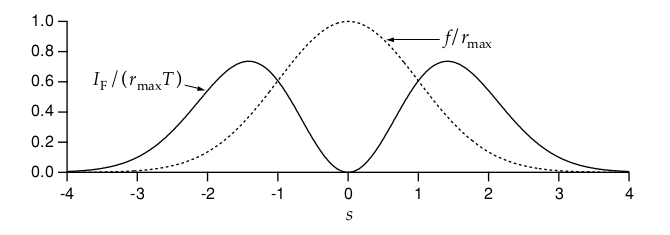
\includegraphics[scale = 0.4]{./png/3-11}
\end{center}
\end{exm}

\begin{rem}
  Individual neurons carry the most Fisher
information in regions of their tuning curves where average firing rates
are rapidly varying functions of the stimulus value, not where the firing
rate is highest.
\end{rem}
\begin{rem}
   The Fisher information can be used to derive an interesting result on the
optimal widths of response tuning curves. Consider a population of neurons with tuning curves of identical shapes, distributed evenly over a
range of stimulus values as in Example \ref{exm:Gaussian tuning curves}. Equation \ref{eq:3.45} indicates that the
Fisher information will be largest if the tuning curves of individual neurons are rapidly varying (making the square of their derivatives large), and
if many neurons respond (making the sum over neurons large). For typical neuronal response tuning curves, these two requirements are in conflict.
If the population of neurons has narrow tuning curves,
individual neural responses are rapidly varying functions of the stimulus,
but few neurons respond. Broad tuning curves allow many neurons to
respond, but the individual responses are not as sensitive to the stimulus
value.
\end{rem}
\begin{exm}
  To determine whether narrow or broad tuning curves produce the
more accurate encodings, we consider a dense distribution of Gaussian
tuning curves, all with $\sigma_a=\sigma_{r}$. Using such curves in
Equation \ref{eq:3.45}, we find
\begin{equation}
  \label{eq:3.46}
  I_{\rm{F}}(s)=T\sum\limits_{a=1}\limits^N
  {\frac{r_{\max}(s-s_{a})^{2}}{\sigma_r^{4}}\exp \left( -\frac{1}{2}\left( \frac{s-s_{a}}{\sigma_{r}} \right)^{2} \right)}.
\end{equation}
\end{exm}

\begin{prop}

This expression can be approximated by replacing the sum over neurons
with an integral over their preferred stimulus values and multiplying by a
density factor $\rho_{s}$. The factor $\rho_{s}$ is the density with which the neurons cover
the range of stimulus values, and it is equal to the number of neurons with
preferred stimulus values lying within a unit range of $s$ values. Replacing
the sum over $a$ with an integral over a continuous preferred stimulus parameter $\xi$ (which replaces $s_{a}$ ), we find
\begin{equation}
  \begin{aligned}
    \label{eq:3.47}
   I_{\rm{F}}(s)&=\rho_{s}T\int_{-\infty}^{\infty}{\frac{r_{\max}(s-\xi)^{2}}{\sigma_r^4}\exp\left(-\frac{1}{2}\left( \frac{s-\xi}{\sigma_r}\right)^{2} \right)}\\
                  &=\frac{\sqrt{2\pi}\rho_{s}\sigma_rr_{\max}T}{\sigma_r^2}.
  \end{aligned}
\end{equation}
The number of neurons that respond to a given stimulus value is
roughly $\rho_{s}\sigma_r$, and the Fisher information is proportional to this number divided by the square of the
tuning curve width seen from Equation \ref{eq:3.47}.Combining these factors, the Fisher information is inversely proportional to $\sigma_{r}$, and the encoding accuracy increases with narrower tuning curves.
\end{prop}

\begin{prop}
  Consider a stimulus with
$D$ parameters and suppose that the response tuning curves are products
of identical Gaussians for each of these parameters. If the tuning curves
cover the $D$-dimensional space of stimulus values with a uniform density $\rho_{s}$, the number of responding neurons for any stimulus value is proportional to $\rho_{s}\sigma_r^{D}$ and, using the same integral approximation as in equation (\ref{eq:3.47}), the Fisher information is
\begin{equation}
  I_{\rm{F}}=\frac{(2\pi)^{D/2}D\rho_{s}\sigma_r^{D}r_{\max}T}{\sigma_r^2}=(2\pi)^{D/2}D\rho_{s}\sigma_r^{D-2}r_{\max}T.
\end{equation}
\end{prop}

\begin{rem}
  The trade-off between the encoding accuracy of individual neurons and the
number of responding neurons depends on the dimension of the stimulus space. Narrowing the tuning curves (making $\sigma_{r}$ smaller) increases the
Fisher information for $D=1$, decreases it for $D > 2$, and has no impact if
$D = 2$.
\end{rem}

\subsection{Optimal Discrimination}
\begin{rem}
   In the first part of this chapter, we considered discrimination between two
values of a stimulus. An alternative to the procedures discussed there is
simply to decode the responses and discriminate on the basis of the estimated stimulus values.
\end{rem}
\begin{prop}
  Consider the case of discriminating between s
and $s+\Delta s$ for small $\Delta s$. For large $N$, the average value of the difference
between the ML estimates for the two stimulus values is equal to
$\Delta s$ (because the estimate is unbiased) and the variance of each estimate (for small
$\Delta s$) is $1/I_{\rm{F}}(s)$ . Thus, the discriminability, defined
in Equation \ref{eq:3.4}, for the ML-based test is
\begin{equation}
  \label{eq:3.49}
  d'=\Delta s \sqrt{I_{\rm{F}}(s)}.
\end{equation}
It can be known that the larger the Fisher information, the higher the discriminability.
\end{prop}

\begin{exc}
  Proof that for small $s$, this discriminability is the same
as that of the likelihood ratio test $Z(\mathbf{r})$ defined in Equation \ref{eq:3.47}.
\end{exc}



\begin{exm}
  The figure makes a comparison of Fisher information and discrimination thresholds for
orientation tuning.The solid curve is the minimum standard deviation of an estimate of orientation angle from the Cramér-Rao bound, plotted as a function of the
number of neurons $(N)$ involved in the estimation. The triangles are data points
from an experiment that determined the threshold for discrimination of
the orientation of line images by human subjects.
\begin{center}
   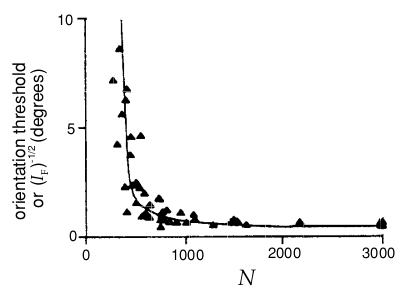
\includegraphics[scale = 0.6]{./png/3-12}
\end{center}
\end{exm}
















%%% Local Variables:
%%% mode: latex
%%% TeX-master: "../notesOnFluidMechanics"
%%% End:



\end{multicols}

%%% Local Variables:
%%% mode: latex
%%% TeX-master: "../notesOnFluidMechanics"
%%% End:


\chapter{Information Theory}
\label{cha:InformationTheory}

\begin{multicols}{2}
\setlength{\columnseprule}{0.2pt}  

\section{1.1}
\label{sec:1.1}

% \begin{defn}
%   The \emph{angular momentum},
%   also called \emph{moment of momentum} $\mathbf{L}$,
%   is the cross product of a moment arm $\mathbf{r}$ and
%   the linear momentum $m \mathbf{V}$ of a fluid particle,
%   i.e.,
%   \begin{equation}
%     \mathbf{L} = \mathbf{r}\times m\mathbf{V}.
%   \end{equation}
% \end{defn}
% \begin{center}
%   \includegraphics[scale=0.45]{./png/angularMomentumDefn}
% \end{center}

\begin{prin}[Conservation of angular momentum]
  \label{prin:angularMomentum}
  The rate of change of angular momentum of a system is equal to
  the net torque acting on the system,
  i.e.,
  \begin{equation}
    \frac{\dif \mathbf{L}}{\dif t} = \boldsymbol\tau,
  \end{equation}
  where $\boldsymbol\tau$ is the torque of all external forces on the system
  about any chosen axis,
  and $\dif \mathbf{L}/\dif t$ is the rate of change of
  angular momentum of the system about the same axis.
\end{prin}

% wo ai song jian jian
% wobuai bu xi zao de songjianjian

%%% Local Variables:
%%% mode: latex
%%% TeX-master: "../notesOnFluidMechanics"
%%% End:


\documentclass[letterpaper,oneside]{book}

\usepackage{geometry}
% make full use of A4 papers
\geometry{margin=1.5cm, vmargin={0pt,1cm}}
\setlength{\topmargin}{-1cm}
\setlength{\paperheight}{29.7cm}
\setlength{\textheight}{25.1cm}

% auto adjust the marginals
\usepackage{marginfix}

\usepackage{amsfonts}
\usepackage{amsmath}
\usepackage{amssymb}
\usepackage{amsthm}
\usepackage{CJKutf8}   % for Chinese characters
\usepackage{enumerate}
\usepackage{graphicx}  % for figures
\usepackage{layout}
\usepackage{multicol}  % multiple columns to reduce number of pages
\usepackage{mathrsfs}  
\usepackage{fancyhdr}
\usepackage{subfigure}
\usepackage{tcolorbox}
\usepackage{tikz-cd}
\usepackage{gensymb}
\usepackage{upgreek}
\usepackage{dsfont}

%------------------
% common commands %
%------------------
\newcommand{\dif}{\mathrm{d}}
\newcommand{\Dim}{\mathrm{D}}
\newcommand{\avg}[1]{\left\langle #1 \right\rangle}
\newcommand{\xibold}{\boldsymbol{\xi}}
\newcommand{\varphibold}{\boldsymbol{\varphi}}
\newcommand{\psibold}{\boldsymbol{\psi}}
\newcommand{\RE}{{\text{Re}}}

% this environment is for solutions of examples and exercises
\newenvironment{solution}%
{\noindent\textbf{Solution.}}%
{\qedhere}
% the following command is for disabling environments
%  so that their contents do not show up in the pdf.
\makeatletter
\newcommand{\voidenvironment}[1]{%
  \expandafter\providecommand\csname env@#1@save@env\endcsname{}%
  \expandafter\providecommand\csname env@#1@process\endcsname{}%
  \@ifundefined{#1}{}{\RenewEnviron{#1}{}}%
}
\makeatother

%----------------------------------------
% theorem and theorem-like environments %
%----------------------------------------
\numberwithin{equation}{chapter}
\theoremstyle{definition}

\newtheorem{thm}{Theorem}[chapter]
\newtheorem{alg}[thm]{Algorithm}
\newtheorem{asm}[thm]{Assumption}
\newtheorem{axm}[thm]{Axiom}
\newtheorem{coro}[thm]{Corollary}
\newtheorem{defn}[thm]{Definition}
\newtheorem{exm}[thm]{Example}
\newtheorem{exc}[thm]{Exercise}
\newtheorem{frm}[thm]{Formula}
\newtheorem{lem}[thm]{Lemma}
\newtheorem{ntn}{Notation}
\newtheorem{prop}[thm]{Proposition}
\newtheorem{rem}{Remark}[chapter]
\newtheorem{rul}[thm]{Rule}
\newtheorem{prin}[thm]{Principle}

\begin{document}
\pagestyle{empty}
\pagenumbering{roman}

%\tableofcontents
%\clearpage

\pagestyle{fancy}
\fancyhead{}
% \lhead{Yang Li}
% \chead{Notes on Fluid Mechanics}
% \rhead{2020}

%\setcounter{chapter}{-1}
\pagenumbering{arabic}
% \setcounter{page}{0}

% --------------------------------------------------------
% uncomment the following to remove these environments 
%  to generate handouts for students.
% --------------------------------------------------------
%\begingroup
%\voidenvironment{rem}%
%\voidenvironment{proof}%
%\voidenvironment{solution}%

% each chapter is factored into a separate file.

\chapter{Neual Encoding:Firing Rates and Spike Statics}
\label{cha:Firing Rates and Spike Statics}

\begin{multicols}{2} 
\setlength{\columnseprule}{0.2pt}  

\section{Spike Trains and Firing Rate}
\label{sec:firing rate}

\subsection{Firing Rate}

\begin{asm}
  Action potentials are typically treated as identical 
  stereotyped events in neural encoding
  studies ignoring in duration, amplitude, and shape. 
  We ignore the brief duration of an action potential (about 1 ms),
  an action potential sequence can be characterized simply by a list of the
  times when spikes occurred.
\end{asm} 

\begin{ntn}
  \emph{Spike train} is represented a list of the times $\{t_i\}_{i=1}^n$ when spikes occurred.
\end{ntn}

\begin{defn}
  \emph{Neural response function} $\rho (t)$ shows whether a spike is fired at time $t$,
   which can be represent as a sum of infinitesimally narrow, 
  idealized spikes in the form of Dirac $\delta$ functions
  \begin{equation}
    \label{equ:1.1}
    \rho(t)=\sum_{i=1}^n\delta(t-t_i),
  \end{equation}
  where $t_i$ with $i=1,2,\dots,n$, recorded in the trail, is the spike train
   %taken to 
   start at time $0$ and end at time $T$, so $0\leq t_i\leq T$ for all $i$.
\end{defn}

\begin{lem}
  $\delta$ function satisfies, for any well-behaved function $h(t)$
  \begin{equation}
    \label{equ:1.3}
    \int \delta(t-\tau)h(\tau)d\tau=h(t),
  \end{equation}
  \begin{proof}
  It follows from
  \begin{equation*}
    %\lim_{\epsilon\rightarrow 0}\int_{-\infty}^{+\infty} \delta(t-\tau)h(\tau)d\tau=
    \lim_{\epsilon\rightarrow 0}\int_{t - \epsilon}^{t + \epsilon} \delta(t-\tau)h(\tau)d\tau
    =h(t)\int_{t - \epsilon}^{t + \epsilon} \delta(t-\tau)d\tau=h(t)
  \end{equation*}
  \end{proof}
which provided that the limits of the integral surround the point $t$ (if they do not,
  the integral is $0$).
\end{lem}

\begin{thm}
  $\rho(t)$ is used to re-express sums over spikes as integrals over time. For any 
  well-behaved function $h(t)$, we can write
  \begin{equation}
    \label{equ:1.2}
    \sum_{i=1}^n h(t-t_i)=\int_{-\infty}^{\infty}h(\tau)\rho(t-\tau)d\tau,
  \end{equation}
  where the integral is over the duration of the trial.
  \begin{proof}
    The equation directly follows Equation \ref{equ:1.3}.
  \end{proof}
\end{thm}

\begin{defn}
  \emph{Spike-count rate $r$} is obtained by counting the number of action potentials that appear during a trial and
  dividing by the duration of the trial,
  \begin{equation}
    r=\frac{n}{T}=\frac{1}{T}\int_0^T\rho(\tau)d\tau.
  \end{equation}
  The second equality follows from the fact that $n=\int\rho(\tau)d\tau$ and indicates
that the spike-count rate is the time average of the neural response function over the 
duration of the trial.
\end{defn}

% \begin{rem}
%   A time-dependent fring rate can be defined by counting spikes over short time intervals, but this can no longer
% be computed from a single trial values. The solution to this problem is to average over multiple trials.
% \end{rem}

\begin{rem}
  The spike-count rate can be determined from a single trial, but at the expense of 
  losing all temporal resolution about variations in the neural response during the 
  course of the trial. A time-dependent firing rate can be defined by counting spikes 
  over short time intervals, but this can no longer
be computed from a single trial.
\end{rem}

\begin{exm}
  We can define the firing rate
at time $t$ during a trial by counting all the spikes that occurred between
times $t$ and $t + \Delta t$, for some small interval $\Delta t$, and dividing this count by
$\Delta t$. However, for small $\Delta t$, which allows for high temporal resolution, the
result of the spike count on any given trial is apt to be either $0$ or $1$, giving
only two possible firing-rate values.
\end{exm}

\begin{ntn}
  We use angle brackets, $\langle\ \rangle $, to denote averages over trials that use the same stimulus.
\end{ntn}

%\begin{exm}
 % The trial-averaged neural response function is denoted by $\langle \rho(t)\rangle $
%\end{exm}

\begin{defn}
  The \emph{time-dependent firing rate} r($t$) is the the average number of spikes (averaged over trials) appearing 
  during a
  short interval between times $t$ and $t+\Delta t$, divided by the duration of
   the interval,
   \begin{equation}
    \label{equ:1.5}
     r(t)=\frac{1}{\Delta t}\int_t^{t+\Delta t}\langle \rho(\tau)\rangle d\tau,
   \end{equation}
   where $\langle\rho(t)\rangle$ is the trial-averaged neural response function.
\end{defn}      

\begin{ntn}
  We use the notation r($t$) opposed to $r$ for the spike-count rate, and use the term 
  “firing rate” without any
modifiers, we mean r($t$).
\end{ntn}

\begin{rem}
  Formally, the limit $\Delta t\rightarrow 0$ should be taken on
the right side of Equation \ref{equ:1.5}, but, in extracting a time-dependent firing
rate from data, the value of $\Delta t$ must be large enough so there are sufficient
numbers of spikes within the interval defining r($t$) to obtain a reliable estimate of the 
average.
\end{rem}

\begin{prop}
  For sufficiently small $\Delta t$, $r(t)\Delta t$ 
  is the probability of a spike occurring during a short interval of duration $\Delta t$ around the time $t$.
  %which is called \emph{spiking probablity}.
  \begin{proof}
  For sufficiently small $\Delta t$, $r(t)\Delta t$ is the average number of spikes occurring
between times $t$ and $t + \Delta t$ over multiple trials. The average number of
spikes over a longer time interval is given by the integral of $r ( t )$ over that
interval. If $t$ is small, there will never be more than one spike within the
interval between $t$ and $t + \Delta t$ on any given trial. This means that $r(t)\Delta t$ is
also the fraction of trials on which a spike occurred between those times.
\end{proof}
\end{prop}



\begin{thm}
  For any function $h$, 
  we can
replace the trial-averaged neural response function with the firing rate r($t$)
within any well-behaved integral.
  \begin{equation}
    \label{equ:1.6}
    \int h(\tau)\langle \rho(t-\tau)\rangle d\tau = \int h(\tau)r(t-\tau)d\tau.
  \end{equation}
\end{thm}

\begin{rem}
  Equation \ref{equ:1.6} establishes an important relationship between the
average neural response function and the firing rate, the two are equivalent when used inside 
integrals. And provides another interpretation of
  r($t$) as the trial-averaged density of spikes along the time axis.
\end{rem}

\begin{defn}
  \emph{Average firing rate $\langle r \rangle $} is the spike-count firing rate to be averaged over trials.
  \begin{equation}
    \label{equ:1.7}
    \langle r\rangle =\frac{\langle n\rangle }{T}
    %=\frac{1}{T}\int_{0}^{T} \langle\rho(\tau) \rangle \,d\tau =\frac{1}{T}\int_{0}^{T}r(t)\,dt
  \end{equation}
   where $\langle n \rangle $ is the trial-averaged number of the spike in the trial, 
   $T$ is the time period of the trial.
\end{defn}

\begin{prop}
  \begin{equation*}
    \langle r\rangle=\frac{1}{T}\int_{0}^{T}r(t)\,dt
  \end{equation*}
  \begin{proof}
    \begin{equation*}
      \langle r\rangle =\frac{\langle n\rangle }{T}
    =\frac{1}{T}\int_{0}^{T} \langle\rho(\tau) \rangle \,d\tau =\frac{1}{T}\int_{0}^{T}r(t)\,dt
    \end{equation*}
    The first equality indicates that $\langle r\rangle $ is just the average 
   number of spikes per trial divided by the trial duration. The third equality follows from
the equivalence of the firing rate and the trial-averaged neural response
function within integrals Equation \ref{equ:1.6}. The average firing rate is equal to
both the time average of r($t$) and the trial average of the spike-count rate $r$. 
  \end{proof}
\end{prop}

\begin{rem}
  Whenever possible, we use the terms “firing rate”, “spike-count rate”
, and “average firing rate” for r($t)$, $r$, and $\langle  r\rangle  $, respectively. In particular, 
we distinguish the spike-count rate $r$
from the time-dependent firing rate r($t$) by
including the time argument in the latter expression (unless r($t)$ is independent of time).
\end{rem}

\subsection{Measuring Firing Rates}

\begin{ntn}
  The firing rate r($t$) cannot be determined exactly from the limited data
available from a finite number of trials. In addition, there is no unique
way to approximate r($t$).
  %In order to determine firing rate r($t$), we will introduce the concept of a linear filter and kernel.
  We illustrate the methods of measuring firing rate by extracting
  firing rates from a single trial, but more accurate results could be obtained
  by averaging over multiple trials.
  \begin{exm}
    We shows $3$s of the response of a neuron in the inferotemporal cortex 
  recorded while a monkey watched a video. Neurons
  in the region of cortex where this recording was made are selective for
  complex visual images, including faces.
  \end{exm}
\end{ntn}
\begin{center}
  \label{fig:1.4A}
    \includegraphics[scale=0.048]{./png/fig:1.4A.jpg}
  \end{center}

\begin{alg}
  A simple algorithm of extracting an estimate of the firing rate from a spike train is to divide time into
discrete bins of duration $\Delta t$, count the number of spikes within each bin,
and divide by $\Delta t$.
\end{alg}

\begin{exm}
  This figure shows the approximate firing rate computed
using this procedure with a bin size of 100 ms. Note that with this procedure, the quantity being computed is 
really the spike-count firing rate over the duration of the bin, and that the firing rate 
r($t$) within a 
given bin is approximated by this spike-count rate. The binning and counting procedure 
illustrated in this figure 
generates an estimate of the firing rate that is a piecewise constant function of time, 
resembling a histogram.
\end{exm}

\begin{center}
  \label{fig:1.4B}
  \includegraphics[scale=0.053]{./png/fig:1.4B.jpg}
\end{center}

\begin{lem}
   Because spike counts can take only integer values, the rates computed by this method will 
   always 
  be integer multiples of $1 / \Delta t$, and thus they take discrete values. Decreasing 
  the value of $\Delta t$
increases temporal resolution by providing an estimate of the firing rate at
more finely spaced intervals of time, but at the expense of decreasing the
resolution for distinguishing different rates.
\end{lem}

\begin{alg}
  One algorithm to avoid quantized
firing rates is to vary the bin size so that a fixed number of spikes appears
in each bin. The firing rate is then approximated as that fixed number of
spikes divided by the variable bin width.
\end{alg}

\begin{rem}
  Counting spikes in preassigned bins produces a firing-rate estimate that
depends not only on the size of the time bins but also on their placement.
\end{rem}

\begin{alg}
To avoid the arbitrariness in the placement of bins, the algorithm is taking
a single bin or window of duration $\Delta t$ and slide it along the spike train,
counting the number of spikes within the window at each location which have a better 
temporal resolution.
\end{alg}

\begin{exm}
  \label{fig:1.4C}
  The jagged curve in  the figure below shows the result of sliding a $100$ ms wide
window along the spike train.  The firing rate approximated in 
this way
can be expressed as the sum of a window function over the times $t_i$ for
$i = 1 , 2 ,\dots, n$ when the $n$ spikes in a particular sequence occurred,
\begin{equation}
  \label{equ:1.8}
  r_{\text{approx}}(t)=\sum_{i = 1}^{n}\omega(t-t_i), 
\end{equation}
where the window function is

\begin{equation}
  \label{equ:1.9}
  \omega(t)=\left\{
    \begin{aligned}
      1/\Delta t \quad &\text{if} -\Delta t/2\leq t\leq \Delta t/2\\
      0 \quad & \text{otherwise}.
    \end{aligned}
  \right.
\end{equation}
The jagged appearance of the curve is caused 
by the discontinuous shape of the window function used.
\end{exm}

\begin{center}
  \includegraphics[scale=0.054]{./png/fig:1.4C.jpg}
\end{center}

\begin{prop}
  The sum in Equation\ref{equ:1.8} can also be written as the integral of the window
function times the neural response function
\begin{equation}
  \label{equ:1.10}
  r_{\text{approx}}(t)=\int_{-\infty}^{\infty}\omega(\tau)\rho(t-\tau)d\tau.
\end{equation}
\begin{proof}
  The proof directly follows Equation\ref{equ:1.2}.
\end{proof}
\end{prop}

\begin{defn}
  The integral in Equation \ref{equ:1.10} is called a \emph{linear filter}, and the window 
  function $\omega$, also called the \emph{filter kernel}, specifies how the neural 
  response function evaluated at time $t-\tau$ contributes to the firing rate approximated 
  at time $t$.
\end{defn}

\begin{exm}
  \label{fig:1.4D}
  Instead of the rectangular window function used in figure in example \ref{fig:1.4C}, 
  figure in example \ref{fig:1.4D} use a 
  continuous window function like the Gaussian
  \begin{equation}
    \label{equ:1.11}
    w(\tau)=\frac{1}{\sqrt{2\pi}}\sigma_{\omega}\text{exp}\left(-\frac{\tau^2}{2\sigma_{\omega}^2} \right),  
  \end{equation}
   which is used in Equation \ref{equ:1.8} generates 
a firing-rate estimate that is a smooth function of time.
In this case, $\sigma_{\omega}$  controls the temporal resolution of the resulting rate, 
playing a role analogous to $\Delta t$.
\end{exm}

\begin{center}
  \includegraphics[scale=0.245]{./png/fig:1.4D.png}
\end{center}

\begin{prin}
  A postsynaptic neuron monitoring the spike train of a presynaptic cell has
access only to spikes that have previously occurred.
\end{prin}

\begin{defn}
  A window function or kernel is called \emph{causal} when an approximation
of the firing rate at time $t$ that depends only on spikes fired before $t$ can
be calculated using a window function that vanishes when its argument is negative.

\end{defn}

\begin{defn}
  The \emph{half-wave rectification} $[z]_+$ for any quantity $z$ stands for,
\begin{equation}
  \label{equ:1.13}
  [z]_+ =\left\{
    \begin{aligned}
      z \quad &\text{if} \quad z\geqslant 0\\
      0 \quad & \text{otherwise}.
    \end{aligned}
  \right.
\end{equation}
\end{defn}

\begin{exm}
  \label{fig:1.4E}
  One commonly used window function is the $\alpha$ function
  \begin{equation}
    w(\tau)=[\alpha^2 \tau \text{exp}(-\alpha\tau) ]_+ 
  \end{equation}
  where $1/\alpha$ determines the temporal resolution of the resulting firing-rate
 estimate. The figure below shows the firing rate approximated by such a causal scheme.
\end{exm}

\begin{center}
  \includegraphics[scale=0.72]{./png/fig:1.4E.png}
\end{center}

\begin{rem}
  Note that the rate computed in example \ref{fig:1.4E} tends to peak later than the 
  rate computed in example \ref{fig:1.4D} using a temporally symmetric window function.%%这个地方需要解释一下吗?
\end{rem}

\subsection{Tuning Curve}

\begin{rem}
  Neuronal responses typically depend on many different properties of a
stimulus. In this chapter, we characterize responses of neurons as functions of 
just one of the stimulus attributes to which they may be sensitive. The value of this 
single attribute is denoted by \emph{s}. In chapter ??, we consider
more complete stimulus characterizations.
\end{rem}

\begin{defn}
  The \emph{neural response tuning curve} is the average firing rate written 
  as a function of $s$, $\langle r\rangle =f(s)$. The functional form of a tuning 
  curve depends on the parameter $s$ used to describe the stimulus. 
  %The precise choice of parameters used as arguments of tuning curve functions is partially a matter of convention.
\end{defn}

\begin{rem}
  A simple way of characterizing the response of a neuron is to count the
number of action potentials fired during the presentation of a stimulus.
This approach is most appropriate if the parameter $s$ characterizing the
stimulus is held constant over the trial. If we average the number of action potentials 
fired over (in theory, an infinite number of) trials and divide by the trial duration, 
we obtain the average firing rate, $ \langle r\rangle$, defined in Equation \ref{equ:1.7}.
\end{rem}

\begin{ntn}
  Because tuning curves correspond to firing rates, they are measured in units of spikes 
  per second or Hz.
\end{ntn}

\begin{exm}
  \label{fig:1.5}
   We show extracellular recordings of a neuron in the primary visual cortex (V1) of 
a monkey. While these recordings were being made, a
bar of light was moved at different angles across the region of the visual
field where the cell responded to light. This region is called the receptive 
field of the neuron. Note that the number of action potentials fired
depends on the angle of orientation of the bar.

The dots in the figure B of example \ref{fig:1.5} indicate the average firing rate depends on the degrees of the orientation angle of the light bar stimulus.

The data have been fitted by a response tuning curve of the form of \emph{Gaussian tuning curve}
\begin{equation}
  \label{equ:1.14}
  f(s)=r_{\text{max}}\text{exp}\left(-\frac{1}{2}\left(\frac{s-s_{\text{max}}}{\sigma_f}\right)^2\right),
\end{equation}

The curve  in figure B is a fit using
the Equation \ref{equ:1.14} with parameters $r_{\text{max}} = 52 . 14 $Hz, $s_{\text{max}}= 0 ^\circ$,
 and $\sigma_f= 14 . 73 ^\circ $,
where $s$ is the orientation angle of the light bar, $s_{\text{max}}$ is the orientation angle
evoking the maximum average response rate $r_{\text{max}}$ (with $s-s_{\text{max}} $ taken 
to lie in the range between $- 90^\circ $ and $+90^\circ$  ), and $\sigma_f$ determines the 
width of the tuning curve. The neuron responds most vigorously when a stimulus
having $s=s_{\text{max}} $ is presented, so we call $s_{\text{max}}$ the preferred orientation angle
of the neuron.

\begin{center}
  \includegraphics[scale=0.38]{./png/fig:1.5.png}
\end{center}
\end{exm}

\begin{rem}
  Tuning curves can also be measured for neurons in motor areas, in which
case the average firing rate is expressed as a function of one or more parameters describing 
a motor action.
\end{rem}

\begin{exm}
  \label{fig:1.6}
  We show an example of extracellular recordings from a neuron in primary motor cortex 
  in a monkey
  that has been trained to reach in different directions. The stacked traces for
  each direction are rasters showing the results of five different trials. The
  horizontal axis in these traces represents time, and each mark indicates
  an action potential. The firing pattern of the cell, in particular the rate at
  which spikes are generated, is correlated with the direction of arm movement.% and thus 
  encodes information about this aspect of the motor action.

  The dots in figure B of example \ref{fig:1.6} indicate the average firing rate depends 
  on the degrees of the direction of the arm movement.
  Here the data points have
  been fitted by a tuning curve in the form of a \emph{cosine tuning curve} to be half-wave 
  rectified.
\begin{equation}
    \label{equ:1.16}
    f(s)=[r_0+\left(r_{\text{max}}-r_0\right)\cos\left(s-s_{\text{max}}\right)]_+.
  \end{equation}

  where $s$ is the reaching angle of the arm, $s_{\text{max}}=161.25^\circ$ is the reaching 
  angle associated with the maximum response $r_{\text{max}}$, and $r_0=32.34$ Hz is an 
  offset or background
  firing rate that shifts the tuning curve up from the zero axis. 
  \begin{center}
    \includegraphics[scale=0.34]{./png/fig:1.6.png}
  \end{center}
\end{exm}

\begin{exm}
  \label{fig:1.7}
  The mode of retinal disparity. The gray lines with arrows show the
location on each retina of an object located nearer than the fixation point F. The
image from the fixation point falls at the fovea in each eye, the small pit where
the black lines meet the retina. The image from a nearer object falls to the left of
the fovea in the left eye and to the right of the fovea in the right eye. For objects
farther away than the fixation point, this would be reversed. The disparity angle $s$
is indicated in the figure.

The dots in figure B of example \ref{fig:1.7} indicate average firing rate of a V1 neuron depends on
retinal disparity and illustrates another important type of tuning curve.

Here the data points have been fitted with a tuning curve called
a logistic or sigmoidal function,
\begin{equation}
  \label{equ:1.17}
  f(s)=\frac{r_{\text{max}}}{1+\exp\left(\left(s_{1/2}-s\right)/\Delta_s\right)}.
\end{equation}
In this case, $s$ is the retinal disparity, the parameter $s_{1/2}$ is the disparity
that produces a firing rate half as big as the maximum value $r_{\text{max}}$ , and $\Delta_s$
controls how quickly the firing rate increases as a function of $s$. If $\Delta_s$ is
negative, the firing rate is a monotonically decreasing function of $s$ rather
than a monotonically increasing function.
\begin{center}
  \includegraphics[scale=0.39]{./png/fig:1.7.png}
\end{center}
\end{exm}

\subsection{Spike-Count Variability}
\begin{rem}
  Tuning curves allow us to predict the average firing rate, but they do not
describe how the spike-count firing rate $r$ varies about its mean value $\langle r\rangle=f(s) $ 
from trial to trial. While the map from stimulus to average
response may be described deterministically, it is likely that single-trial
responses such as spike-count rates can be modeled only in a probabilistic manner.
Generally, $r$ values can be generated from a probability
distribution with mean $f(s)$.
\end{rem}

\begin{defn}
  The trial-to-trial deviation of $r$ from $f ( s )$ is
considered to be noise, and such models are often called \emph{noise models}.
\end{defn}
\begin{defn}
  The standard deviation for the noise distribution either can be independent of 
  $f ( s )$, in which case is called \emph{additive noise}, or it can
depend on $f ( s )$. \emph{Multiplicative noise} corresponds to having the standard
deviation proportional to $f ( s )$.
\end{defn}



%\bibliography{bib/numericalApprox}
%\bibliographystyle{abbrv}
%\bibliographystyle{abbrvnat}
%\setcitestyle{authoryear,open={[},close={]}}
\end{multicols}
\end{document}


%%% Local Variables: 
%%% mode: latex
%%% TeX-master: t
%%% End: 


\section{Population Decoding}
\label{sec:Population Decoding}

\begin{rem}
  The use of large numbers of neurons to represent information is a basic
operating principles of many nervous systems. \emph{Population coding} has a
number of advantages, including reduction of uncertainty due to neuronal
variability and the ability to represent a number of different
stimulus attributes simultaneously. In the previous section, we
discussed discrimination between stimuli on the basis of the response of
a single neuron. The responses of a population of neurons can also be
used for discrimination, with the only essential difference being that terms
such as $p[r|s]$ are replaced by $p[\mathbf{r}|s]$, the conditional
probability density of the population response $\mathbf{r}$. ROC
analysis, likelihood ratio tests, and the Neyman-Pearson lemma continue to apply in exactly the same way.
\end{rem}

\begin{rem}
  \emph{Discrimination} is a special case of decoding in which only a
  few different stimulus values are considered. A more general problem
  is the extraction of a continuous stimulus parameter from one or
  more neuronal responses. In this section, we study how the value of a continuous parameter associated with a static stimulus can be decoded from the spike-count firing
rates of a population of neurons.
\end{rem}

\subsection{Encoding and Decoding Direction}
\begin{exm}
  The cercal system of the cricket, which senses the direction of incoming air
currents is an interesting example of population coding involving a
four interneurons. The figure shows average firing-rate tuning curves
for the four relevant interneurons as a function of wind
direction, which are well approximated by halfwave rectifed cosine
function. The preferred directions of the neurons are located $90^{\circ}$ from each other, and $r_{\max}$
values are typically around 40 Hz.
\end{exm}

\begin{center}
  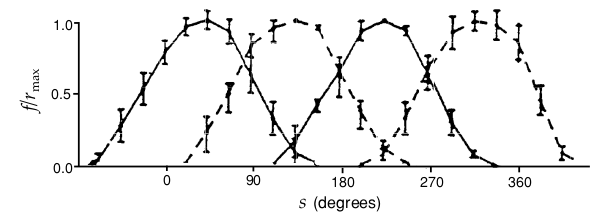
\includegraphics[scale = 0.4]{./png/3-4}
\end{center}

\begin{prop}
  \label{prop:single neuron cosine function}
  Neuron $a$ (where $a=1,2,3,4$) responds
with a maximum average firing rate when the angle of the wind direction
is $s_{a}$, the preferred-direction angle for that neuron. The tuning curve for
interneuron a in response to wind direction $s$, $\left\langle r_{a}
\right\rangle=f_a(s)$, normalized to its maximum, can be written as
\begin{equation}
  \label{eq:3.20}
  \Big( \frac{f(s)}{r_{\max}} \Big)_{a}=[(\cos(s-s_a))]_+,
\end{equation}
where the half-wave rectifcation eliminates negative firing rates. Here
$r_{\max}$, which may be different for each neuron, is a constant equal to the
maximum average firing rate.
\end{prop}

\begin{prop}
 For  the cercal system of the cricket, Equation \ref{eq:3.20} can be written as
  \begin{equation}
  \label{eq:3.21}
 \Big( \frac{f(s)}{r_{\max}} \Big)_{a}=[\vec{v}\cdot\vec{c}_a].
\end{equation}
where spatial vector $\vec{v}$ pointing parallel to the wind velocity in place of the angle
$s$ and having unit length $\big| \vec{v} \big|=1$ and a vector
  $\vec{c}_{a}$  of unit length is the preferred wind direction  pointing in the
  direction specified by the angle $s_{a}$ for each interneuron.

\begin{proof}
In this case, we can use the vector dot product to write
$\cos(s-s_a)=\vec{v}\cdot\vec{c}_a$. In terms of these
vectors, the average firing rate is proportional to a half-wave
rectified projection of the wind direction vector onto the
preferred direction axis of the neuron. And combined with the above
proposition \ref{prop:single neuron cosine function}, we give the answer.
\end{proof}

\end{prop}

\begin{rem}
  Decoding the cercal system is particularly easy because of the close relationship between the representation of wind direction it provides and a
two-dimensional Cartesian coordinate system. The preferred directions
of the four interneurons, like the $x$ and $y$ axes of a Cartesian coordinate
system, lie along two perpendicular directions. Four neurons
are required, rather than two, because firing rates cannot represent negative projections.
\end{rem}

\begin{prop}
  If $r_{a}$ is the spike-count fring rate of neuron $a$, an estimate of
  the wind direction on any given trial can be obtained from the
  direction of the vector
  \begin{equation}
    \label{eq:3.22}
    \vec{v}_{\rm{pop}}=\sum\limits_{a=1}^4\left( \frac{r}{r_{\max}} \right)_a\vec{c}_a.
  \end{equation}
  This vector is known as the \emph{population vector}, and the associated decoding
  method is called the \emph{vector method}. In fact, this encoding is
  the one that requires the least number of neurons to encode
  two-dimensional directions.
\end{prop}

\begin{exm}
In figure A, preferred directions of four cercal interneurons in relation to the
cricket’s body. The firing rate of each neuron for a fixed wind speed is proportional to the projection of the wind velocity vector $\vec{v}$ onto the preferred-direction
axis of the neuron. The projection directions
$\vec{c}_{1}$, $\vec{c}_{2}$, $\vec{c}_{3}$, and $\vec{c}_{4}$ for the four neurons
are separated by  $90^{\circ}$, and they collectively form a Cartesian coordinate system.
In figure B, the root-mean-square error in the wind direction determined by vector decoding of the firing rates of four cercal interneurons. These results were obtained
through simulation by randomly generating interneuron responses to a variety of
wind directions, with the average values and trial-to-trial variability of the firing
rates matched to the experimental data. The generated rates were then decoded
using Equation \ref{eq:3.22} and compared to the wind direction used
to generate them.
   \begin{center}
    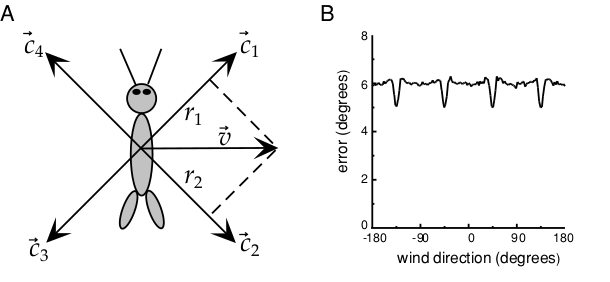
\includegraphics[scale = 0.4]{./png/3-5}
    \label{fig:3.5AB}
  \end{center}
  \end{exm}

\begin{exm}
  As discussed in chapter \ref{cha:Neural Encoding I}, tuning curves of certain neurons in the primary
motor cortex (M1) of the monkey can be described by cosine functions of
arm movement direction. Thus, a vector decomposition similar to that
of the cercal system appears to take place in M1. Many M1 neurons have
nonzero offset rates, $r_{0}$. When an arm movement is made in the direction represented by a vector of unit length, $\vec{v}$, the average fring rates for such a M1
neuron, labeled by an index $a$, can be written as
\begin{equation}
  \label{eq:3.23}
  \left( \frac{\left\langle r \right\rangle-r_{0} }{r_{\max}}\right)_{a}=\left( \frac{f(s)-r_{0}}{r_{\max}} \right)_{a}=\vec{v}\cdot\vec{c}_a,
\end{equation}
where $\vec{c}_a$ is the preferred-direction vector that defines the
selectivity of the neuron. Unlike the cercal interneurons, M1 neurons
do not have orthogonal preferred directions that form a Cartesian
coordinate system. Instead, the preferred directions of the neurons appear to point in all directions with
roughly equal probability.
\end{exm}

\begin{prop}
  If the preferred directions point uniformly in all directions and
  the number of neurons $N$ is suffciently large, the population vector
  \begin{equation}
      \label{eq:3.24}
    \vec{v}_{\rm{pop}}=\sum\limits_{a=1}^N \left( \frac{r-r_{0}}{r_{\max}} \right)_a\vec{c}_a,
  \end{equation}
will, on average, point in a direction parallel to the arm movement direction vector $\vec{c}$. If we average Equation \ref{eq:3.24} over
trials and use Equation \ref{eq:3.23}, we find
\begin{equation}
  \label{eq:3.25}
  \left\langle  \vec{v}_{\rm{pop}} \right\rangle=\sum_{a=1}^N{(\vec{v}\cdot\vec{c}_a)\vec{c}_a},
\end{equation}
 where $\vec{v}_{\rm{pop}}$ is approximately parallel
to $\vec{v}$ if a large enough number of neurons is included in the sum, and
if their preferred-direction vectors point randomly in all directions with
equal probability.
\end{prop}

\subsection{Optimal Decoding Methods}

\begin{rem}
  The vector method is a simple decoding method that can perform quite
well in certain cases, but it is neither a general nor an optimal way
to reconstruct a stimulus from the fring rates of a population of
neurons. In
this section, we dicuss two methods, that are Bayesian inference and MAP
inference, which are considered optimal by some measure.
\end{rem}

\begin{rem}
  \emph{Bayesian} and \emph{MAP} estimates use the conditional
  probability that a stimulus parameter takes a value between $s$ and
  $s+\nabla s$, given that the set of $N$ encoding neurons fired at
  rates given by $\mathbf{r}$. The probability density needed for a
  continuous stimulus parameter, $p[s|\mathbf{r}]$, can be obtained from
  the encoding probability density $p[\mathbf{r}|s]$ by the continuous version of Bayes
theorem,
\begin{equation}
  \label{eq:3.26}
  p[s|\mathbf{r}]=\frac{p[\mathbf{r}|s]p[s]}{p[\mathbf{r}]}.
\end{equation}
A disadvantage of these methods is that extracting $p[s|\mathbf{r}]$ from experimental data can be diffcult.
\end{rem}

\begin{defn}
  Below are the two optimal ways to reconstruct a stimulus from the
  fring rates of a population of neurons:
  \begin{enumerate}[(i)]
  \item The \emph{Bayesian inference} involves finding the minimum of a loss
  function $L(s,s_{\rm{bayes}})$ that quantifyes the cost of reporting
  the estimate $s_{\rm{bayes}}$ when the correct answer is $s$.
  \item  The \emph{MAP inference} chooses the stimulus value, $s_{\rm{MAP}}$,
  that maximizes the conditional probability density of the stimulus,
  $p[s_{\rm{MAP}}|\mathbf{r}]$ and \emph{ML inference} chooses
  $s_{\rm{ML}}$ to maximize the likelihood function,
  $p[\mathbf{r}|s_{\rm{ML}}]$, which generally produce estimates
  that are as accurate, in terms of the variance of the estimate, as
  any that can be achieved by a wide class of estimation methods
  (so-called unbiased estimates).
  \end{enumerate}
\end{defn}

\begin{rem}
  The value of $s_{\rm{bayes}}$ is chosen to minimize the expected
loss averaged over all stimuli for a given set of rates, that is, to minimize
the function $\int L(s,s_{\rm{bayes}})p[s|\mathbf{r}]ds$.
\end{rem}

\begin{exm}
  If the loss function is the squared difference between the estimate
  and the true value, $ L(s,s_{\rm{bayes}})=(s-s_{\rm{bayes}})^{2}$, the
  estimate that minimizes the expected loss is the mean
  \begin{equation}
    \label{eq:3.27}
    s_{\rm{bayes}}=\int p[s|\mathbf{r}]ds.
  \end{equation}
\end{exm}

\begin{exm}
 If the loss function is the absolute value of the
 difference, $L(s,s_{\rm{bayes}})=\big|s-s_{\rm{bayes}} \big|$, then
 $s_{\rm{bayes}}$ is the median rather than the mean of the
 distribution $p[s|\mathbf{r}]$.
\end{exm}


\begin{rem}
  The MAP approach is thus to choose as the estimate $s_{\rm{MAP}}$ the most
  likely stimulus value for a given set of rates. If the prior or
  stimulus probability density $p[s]$ is independent of $s$, then
  $p[s|\mathbf{r}]$ and $p[\mathbf{r}|s]$ have the same dependence on
  $s$, because the factor $p[s]/p[\mathbf{r}]$ in Equation \ref{eq:3.26} is independent of $s$. In this case, the MAP algorithm is equivalent to  maximum likelihood (ML) inference.
\end{rem}

\begin{exm}
  The root-mean-squared difference between
the true and estimated wind directions for the cercal system, using ML
and Bayesian methods is shown as follows. The Bayesian estimate in figure is based on the squared-difference loss function. Both
estimates use a constant stimulus probability density $p[s]$, so the ML and
MAP estimates are identical. The Bayesian result has a slightly
smaller average error across all angles. The dips in the error curves in figure
appear at angles where one tuning curve peaks and two others rise from
threshold. These dips are due to the two
neurons responding near threshold, not to the maximally responding neu-
ron. They occur because neurons are most sensitive at points where their
tuning curves have maximum slopes, which in this case is near threshold.
\begin{center}
  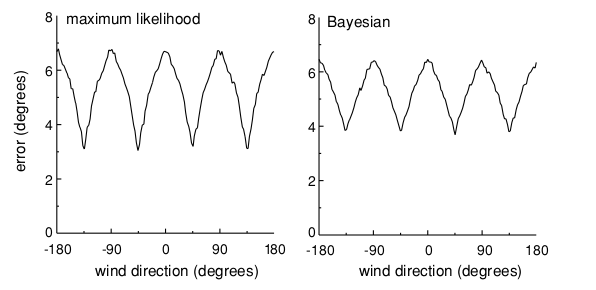
\includegraphics[scale = 0.4]{./png/3-7}
\end{center}
\end{exm}


\begin{exm}
  \label{exm:Gaussian tuning curves}
  Up to now, we have considered the decoding of a direction angle. We now
turn to the more general case of decoding an arbitrary continuous stimulus
parameter. An instructive example is provided by an array of $n$ neurons
with preferred stimulus values distributed uniformly across the full range
of possible stimulus values. An example of such an array for Gaussian
tuning curves,
\begin{equation}
  \label{eq:3.28}
  f_a(s)=r_{\rm{max}}\exp\left(-\frac{1}{2}\left(
      \frac{s-s_{a}}{\sigma_{a}} \right)^{2}\right).
\end{equation}
In this example, each neuron has a tuning curve
with a different preferred value $s_{a}$ and potentially a different
width $\sigma_{a}$. If the tuning curves are evenly and densely distributed across the range of $s$ values, the
sum of all tuning curves
$\sum f_a(s)$ is approximately independent of $s$. The roughly flat line is proportional to this sum.
\begin{center}
  \label{fig:3-8}
  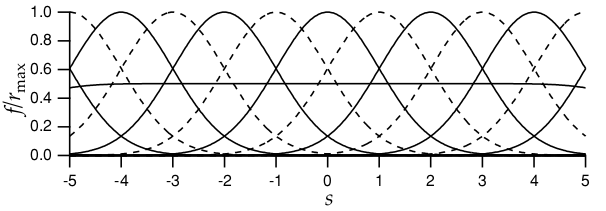
\includegraphics[scale = 0.4]{./png/3-8}
\end{center}
\end{exm}

\begin{rem}
  To implement the Bayesian, MAP, or ML approach, we need to
know the conditional firing-rate probability density $p[\mathbf{r}|s]$ that describes
this variability.
\end{rem}

\begin{prop}
  \label{prop:conditional firing-rate probability density}
  We assume that the firing rate $r_{a}$ of neuron $a$ is determined
by counting $n_{a}$ spikes over a trial of duration $T$ (so that $r_{a} = n_{a}/T$), and
that the variability can be described by the homogeneous Poisson model
discussed in chapter \ref{cha:Neural Encoding I}. In this case, the probability of stimulus s evoking
$n_{a}=r_{a}T$ spikes, when the average firing rate is $\left\langle
  r_{a} \right\rangle=f_a(s)$, is given by
\begin{equation}
  \label{eq:3.29}
  P[r_a|s]=\frac{(f_a(s)T)^{r_aT}}{(r_aT)!}\exp(-f_{a}(s)T).
\end{equation}
If we assume that each neuron fires independently, the firing-rate
probability for the population is the product of the individual
probabilities,
\begin{equation}
  \label{eq:3.30}
   P[\mathbf{r}|s]=\prod\limits_{a=1}\limits^{N}{\frac{(f_a(s)T)^{r_{a}T}} {(r_aT)!}\exp(-f_{a}(s)T)}.
\end{equation}
\end{prop}

\begin{exm}
  The filled circles in figure show a set of randomly generated firing rates
for the array of Gaussian tuning curves for $s=0$ shown above. This figure
also illustrates a useful way of visualizing population responses: plotting
the responses as a function of the preferred stimulus values. The dashed
curve is the tuning curve for the neuron with $s_{a}=0$. Because
the tuning curves are functions of $\left| s-s_{a} \right|$, the values of the dashed curve at
$s_{a}=-5,-4,\dots,5$ are the mean activities of the cells with preferred values
at those locations for a stimulus at $s=0$.
\begin{center}
    \label{fig:3-9}
  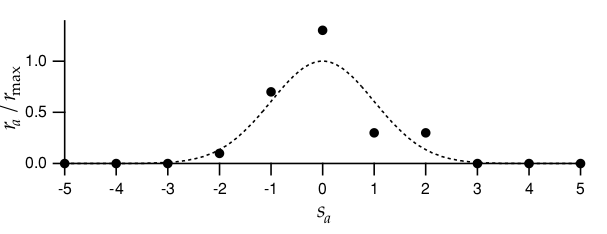
\includegraphics[scale = 0.4]{./png/3-9}
\end{center}
\end{exm}

\begin{prop}
  The ML estimated stimulus, $s_{ML}$, is the stimulus that maximizes $P[\mathbf{r}|s]$. We
find that $s_{\rm{ML}}$ is determined by
\begin{equation*}
  T\sum\limits_{a=1}\limits^{N}{r_{a}\frac{f_{a}'(s_{ML})}{f_{a}(s_{ML})}}=0,
\end{equation*}
where the prime denotes a derivative.
\begin{proof}
 To apply the ML estimation algorithm, we only need to consider the terms
in $P[\mathbf{r}|s]$ that depend on $s$. Because Equation
\ref{eq:3.30} involves a product, it is convenient to take its logarithm and write
\begin{equation}
  \label{eq:3.31}
  \ln P[\mathbf{r}|s]=T\sum\limits_{a=1}\limits^{N}{r_{a}\ln \left( f_a(s) \right)}+\dots,
\end{equation}
where the ellipsis represents terms that are independent
or approximately independent of $s$, including, as discussed above,
$\sum{f_a(s)}$.
 Setting the derivative to $0$, we give the answer.
 \end{proof}
\end{prop}

\begin{exm}
  If the tuning curves are the Gaussians of Equation \ref{eq:3.28},
  this equation can be solved explicitly using the result
  $f_{a}'(s)/f_a(s)=(s_{a}-s)/\sigma_{a}^{2}$,
    \begin{equation}
      \label{eq:3.33}
      s_{\rm{ML}}=\frac{\sum{r_as_a/\sigma_{a}^{2}}}{\sum{r_a/\sigma_{a}^{2}}}.
    \end{equation}
    If all the tuning curves have the same width, this reduces to
    \begin{equation}
      \label{eq:3.34}
      s_{\rm{ML}}=\frac{\sum{r_as_a}}{\sum{r_a}},
  \end{equation}
  which is a simple estimation formula with an intuitive interpretation as
the firing-rate weighted average of the preferred values of the encoding
neurons.
\end{exm}

\begin{rem}
  Although the stimuli obtained by maximum likelihood estimation are
  the weighted average of the best responses. This result looks very
  good, but under the influence of noise, this method may reduce the
  accuracy. The MAP algorithm allows us to include prior knowledge $p[s]$
about the distribution of stimulus values in the decoding estimate. When using
  MAP, The objective function will have one more term $\log(p[s])$
  and the maximum value can still be obtained by derivation. If the
  $p[s]$ is constant, the MAP and ML estimates are
  identical.

   Inaddition, if many neurons are observed, or if a small
  number of neurons is observed over a long trial period, even a
  nonconstant stimulus distribution has little effect and $s_{\rm{MAP}}\approx s_{\rm{ML}}$.
\end{rem}

\begin{prop}
  The MAP estimate is computed from the distribution $p[s|\mathbf{r}]$ determined by
Bayes theorem. In terms of the logarithms of the probabilities, $\ln
p[s|\mathbf{r}]=\ln p[\mathbf{r}|s]+\ln p[s]-\ln P[r]$. The last
term in this expression is independent of $s$ and can be absorbed into the ignored $s$-independent terms, so we can
write, as in Equation \ref{eq:3.31},
\begin{equation}
  \label{eq:3.35}
 \ln p[s|\mathbf{r}]=T\sum\limits_{a=1}\limits^{N}{r_{a}\ln \left(
     f_a(s) \right)+\ln p[s]+\dots}.
 \end{equation}
 Maximizing this determines the MAP estimate,
 \begin{equation}
   \label{eq:3.36}
    T\sum\limits_{a=1}\limits^{N}{\frac{r_{a}f_{a}'(s_{\rm{MAP}})}{f_{a}(s_{MAP})}}+\frac{p'[s_{\rm{MAP}}]}{p[s_{\rm{MAP}}]}=0.
 \end{equation}
\end{prop}

\begin{exm}
  If the stimulus or prior distribution is itself Gaussian with mean
  $s_{\rm{prior}}$  and
variance  $\sigma_{\rm{prior}}$ , and we use the Gaussian array of tuning curves,
Equation \ref{eq:3.36} yields
\begin{equation}
  \label{eq:3.37}
s_{\rm{MAP}}=\frac{T\sum{r_as_a}/\sigma_a^{2}+s_{\rm{prior}}/\sigma_{{\rm{prior}}}^{2}}{T\sum{r_a/\sigma_a^{2}}+1/\sigma_{{\rm{prior}}}^{2}}.
\end{equation}
\end{exm}

\begin{exm}
  The figure compares the conditional stimulus probability densities $p[s|\mathbf{r}]$
for a constant stimulus distribution (solid curve) and for a Gaussian stimulus distribution with $s_{\rm{prior}}=-2$ and $\sigma_{{\rm{prior}}}=1$, using the firing rates given
by the filled circles in last figure. If the stimulus distribution is constant,
$p[s|\mathbf{r}]$ peaks near the true stimulus value of $0$. The effect of a noncon-
stant stimulus distribution is to shift the curve toward the value $-2$, where
the stimulus probability density has its maximum, and to decrease its
width by a small amount. The estimate is shifted to the left because the
prior distribution suggests that the stimulus is more likely to take
negative values than positive ones, independent of the evoked
response. The decreased width is due to the added information that the prior distribution provides.

\begin{center}
    \label{fig:3-10}
  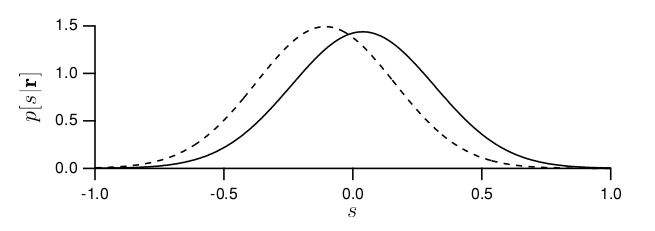
\includegraphics[scale = 0.4]{./png/3-10}
\end{center}
\end{exm}


\begin{defn}
  \label{defn:bias}
  The accuracy with which an estimate $s_{\rm{est}}$ describes a
  stimulus $s$ can be characterized by two important quantities, its
  bias $b_{\rm{est}}(s)$ and its variance
$\sigma_{\rm{est}}^{2}(s)$. The bias is the difference between the
average of $s_{\rm{est}}$ across trials that use the stimulus $s$ and the true
value of the stimulus (i.e., $s$),
\begin{equation}
  \label{eq:3.38}
  b_{\rm{est}}(s)=\left\langle s_{\rm{est}} \right\rangle-s.
\end{equation}
\end{defn}

\begin{defn}
  An estimate is termed unbiased if $b_{\rm{est}}(s)=0$ for all stimulus values.
\end{defn}

\begin{defn}
  The variance of the estimator, which quantifies how much the estimate
  varies about its mean value, is defined as
  \begin{equation}
    \label{eq:3.39}
    \sigma_{\rm{est}}^{2}(s)=\left\langle (s_{\rm{est}} -\left\langle s_{\rm{est}}  \right\rangle)^{2} \right\rangle.
  \end{equation}
\end{defn}

\begin{prop}
  The bias and variance can be used to compute the trial-average
  squared estimation error, $\left\langle (s_{\rm{est}} -s)^{2}\right\rangle$. This is a measure of the spread of the estimated values about the true value of the stimulus. Considering Definition \ref{defn:bias}, we can write the squared estimation error as
    \begin{equation}
      \label{eq:3.40}
      \left\langle (s_{\rm{est}} -s)^{2} \right\rangle=\left\langle (s_{\rm{est}} -\left\langle s_{\rm{est}}  \right\rangle+ b_{\rm{est}}(s))^{2} \right\rangle=\sigma_{\rm{est}}^{2}(s)+b_{\rm{est}}^{2}(s).
    \end{equation}
    In other words, the average squared estimation error is the sum of the
variance and the square of the bias. For an unbiased estimate, the average
squared estimation error is equal to the variance of the estimator.
\end{prop}

\begin{rem}
  In general, minimizing the decoding error in Equation
  \ref{eq:3.40} involves a trade-off between minimizing the bias and
  minimizing the variance of the estimator.
\end{rem}

\subsection{Fisher Information}
\begin{rem}
  Decoding can be used to limit the accuracy with which a neural system
encodes the value of a stimulus parameter because the encoding accuracy
cannot exceed the accuracy of an optimal decoding method.
\end{rem}

\begin{defn}
  The \emph{Fisher
information} is a quantity that provides one such measure of encoding
accuracy. Through a bound known as the \emph{Cramér-Rao bound}, the Fisher
information limits the accuracy with which any decoding scheme can extract an estimate of an encoded quantity.
\end{defn}
\begin{prop}
  The Cramér-Rao lower bound for an estimator $s_{\rm{est}}$ is based on the Cauchy-
  Schwarz inequality, which states that for any two quantities A and B,
  \begin{equation}
    \label{eq:3.67}
    \langle A^2\rangle \langle B^2\rangle\geq\langle AB\rangle^2.
    \end{equation}

\begin{proof}
 Note that
\begin{equation}
  \left\langle\left(\langle B^2\rangle A-\langle
AB\rangle B\right)^2\right\rangle\geq0
\label{eq:3.68}
\end{equation}
because it is the average value of a square. Computing the square
gives
\begin{equation}
\langle B^2\rangle^2\langle A^2\rangle-\langle AB\rangle^2\langle B^2\rangle\geq0
\label{eq:3.69}
\end{equation}
from which the inequality follows directly.
\end{proof}
\end{prop}

\begin{prop}
  The \emph{Cramér-Rao bound} limits the variance of any estimate $s_{\rm{est}}$
  according to
  \begin{equation}
    \label{eq:3.41}
     \sigma_{\rm{est}}^{2}(s)\geq \frac{\left( 1+b_{\rm{est}}'(s) \right)^{2}}{I_{\rm{F}}(s)},
   \end{equation}
   where $b_{\rm{est}}'(s)$ is the derivative of $b_{\rm{est}}(s)$ and $I_{\rm{F}}(s)$ is the Fisher
   information.

\begin{proof}
Consider the inequality of Equation \ref{eq:3.67}
   with $A=\partial \ln p/\sigma_{\rm{est}}^{2}$
   The Cauchy-Schwarz inequality then gives
\begin{equation}
\sigma_{\rm{est}}^2(s)I_F\geq\left\langle\frac{\partial \ln p[\mathbf{r}|s]}{\partial s}(s_{\rm{est}}-\langle s_{\rm{est}}\rangle)\right\rangle^2.
\label{eq:3.70}
\end{equation}
To evaluate the expression on the right side of the inequality \ref{eq:3.70}), we differentiate the defining equation for the bias (Equation \ref{eq:3.38}),
  \begin{equation}
s+b_{\rm{est}}(s)=\langle s_{\rm{est}}\rangle=\int p[\mathbf{r}|s]s_{\rm{est}}d\mathbf{r},
\label{eq:3.71}
\end{equation}
with respect to $s$ to obtain
\begin{equation}
\begin{aligned}
1+b_{\rm{est}}^{'}(s)&=\int\frac{\partial p[\mathbf{r}|s]}{\partial s}s_{\rm{est}}d\mathbf{r}\\
&=\int p[\mathbf{r}|s]\frac{\partial\ln p[\mathbf{r}|s]\partial}{\partial s}s_{\rm{est}}d\mathbf{r}\\
&=\int p[\mathbf{r}|s]\frac{\partial\ln p[\mathbf{r}|s]\partial}{\partial s}(s_{\rm{est}}-\langle s_{\rm{est}}\rangle).
\end{aligned}
\label{eq:3.72}
\end{equation}
The last equality follows from the identity
\begin{equation}
\int p[\mathbf{r}|s]\frac{\partial\ln p[\mathbf{r}|s]}{\partial s}\langle s_{\rm{est}}\rangle d\mathbf{r}=\langle s_{\rm{est}}\rangle\int\frac{\partial p[\mathbf{r}|s]}{\partial s}d\mathbf{r}=0,
\label{eq:3.73}
\end{equation}
because $\int p[\mathbf{r}|s]d\mathbf{r}=1$. The last line of equation  \ref{eq:3.72} is just another way
of writing the expression being squared on the right side of the inequality
\ref{eq:3.70}, so combining this result with the inequality gives
\begin{equation}
\sigma_{\rm{est}}^2(s)I_F\geq(1+b_{\rm{est}}^{'}(s))^2,
\label{eq:3.74}
\end{equation}
which, when rearranged, is the Cramér-Rao bound of Equation \ref{eq:3.41}.
\end{proof}
\end{prop}

\begin{prop}
  If we assume here that the firing rates take continuous values and
  that their distribution in response to a stimulus $s$ is described
  by the conditional probability density $p[\mathbf{r}|s]$(assuming
  the latter is sufficiently smooth) by, $I_{\rm{F}}(s)$ can be written as
\begin{equation}
  \label{eq:3.42}
  I_{\rm{F}}(s)=\left\langle
    -\frac{\partial^{2}\ln p[\mathbf{r}|s]}{\partial s^{2}}
  \right\rangle=\int p[\mathbf{r}|s]\left( -\frac{\partial^{2}\ln p[\mathbf{r}|s]}{\partial s^{2}} \right)d\mathbf{r},
\end{equation}
We can verify that the Fisher information can also be written as
\begin{equation}
  \label{eq:3.43}
  \left\langle \left( \frac{\partial\ln p[\mathbf{r}|s]}{\partial s} \right)^{2}
  \right\rangle=\int p[\mathbf{r}|s]\left( \frac{\partial\ln p[\mathbf{r}|s]}{\partial s} \right)^{2}d\mathbf{r}.
\end{equation}
\end{prop}

\begin{rem}
  As Equation \ref{eq:3.42} shows, the Fisher information is a measure of the expected curvature of the log likelihood at the stimulus value
$s$. Curvature is important because the likelihood is expected to be at
a maximum near the true stimulus value $s$ that caused the
responses. Therefore, we can get two cases:
\begin{enumerate}[(i)]
\item If the likelihood is very curved, and thus the Fisher information is
large, responses typical for the stimulus $s$ are much less likely to
occur for slightly different stimuli. Therefore, the typical response
provides a strong indication of the value of the stimulus.
\item If the
likelihood is fairly flat, and thus the Fisher information is small,
responses common for $s$ are likely to occur for slightly different
stimuli as well. Thus, the response does not as clearly determine the stimulus value.
\end{enumerate}
\end{rem}

\begin{rem}
  The Fisher information is purely local in the sense that it
does not reflect the existence of stimulus values completely different from
$s$ that are likely to evoke the same responses as those evoked by $s$ itself.
\end{rem}

\begin{rem}
  The Cramér-Rao bound sets a limit on the accuracy of any unbiased estimate of the stimulus. When $b_{\rm{est}}(s)=0$, Equation
\ref{eq:3.40} indicates that the average squared estimation error is
equal to $\sigma_{\rm{est}}^{2}$ and, by Equation \ref{eq:3.41}, this
satisfies the bound $\sigma_{\rm{est}}^{2} \geq
1/I_{\rm{F}}(s)$. Provided that we restrict ourselves to unbiased
decoding schemes, the Fisher information sets an absolute limit on
decoding accuracy, and it thus provides a useful limit on encoding
accuracy. In some cases, biased schemes may produce more accurate
results than unbiased ones. For a biased estimator, the average
squared estimation error and the variance of the estimate are not
equal, and the estimation error can be either larger or smaller than $1/I_{\rm{F}}(s)$ .
\end{rem}

\begin{rem}
  The limit on decoding accuracy set by the Fisher information can be
  attained by a decoding scheme we have studied, the maximum
  likelihood method. In the limit of large numbers of encoding
  neurons, and for most firing-rate distributions, the ML estimate is unbiased and saturates the
Cramér-Rao bound.
\end{rem}

\begin{defn}
  \label{defn:efficient estimator}
  Any unbiased estimator that saturates the Cramér-Rao lower bound is
  called efficient, i.e.
  \begin{equation}
    \sigma_{\rm{est}}^{2} =1/I_{\rm{F}}(s).
  \end{equation}
\end{defn}
\begin{thm}
 $I_{\rm{F}}(s)$ grows linearly with $N$, and the ML estimate obeys a
central limit theorem, so that $N^{1/2}(s_{\rm{ML}}-s)$ is Gaussian
distributed with a variance that is independent of $N$ in the large
$N$ limit. In the limit
$N \rightarrow \infty$, the ML estimate is asymptotically consistent, in the sense that
$P[|s_{\rm{ML}}-s|>\varepsilon]\rightarrow 0$ for any $\varepsilon >0$.
\end{thm}

\begin{exm}
  The Fisher information for a population of neurons with uniformly
  arrayed tuning curves (the Gaussian array in example \ref{exm:Gaussian tuning curves} for example) and
Poisson statistics can be computed from the conditional firing-rate probability in Equation \ref{eq:3.31}. Because the spike-count rate is
described here by a probability rather than a probability density, we
use the discrete analog of Equation \ref{eq:3.42},
\begin{equation}
  \label{eq:3.44}
  I_{\rm{F}}(s)=\left\langle
    -\frac{\partial^{2}\ln p[\mathbf{r}|s]}{\partial s^{2}}
  \right\rangle=T\sum\limits_{a=1}\limits^N {\left\langle r_{a} \right\rangle{\left(\left( \frac{f_a'(s)}{f_a(s)} \right)^{2}-\frac{f_a''(s)}{f_a(s)}\right)}}.
  \end{equation}
If we assume that the array of tuning curves is symmetric, like the Gaussian array in example \ref{exm:Gaussian tuning curves}, the second term
in the parentheses of the last expression sums to $0$. We can also
make the replacement $\left\langle r_{a}
\right\rangle=f_a(s)$, producing the final result
\begin{equation}
  \label{eq:3.45}
  I_{\rm{F}}(s)=T\sum\limits_{a=1}\limits^N \frac{f_a'(s)^{2}}{f_a(s)}.
\end{equation}
In this expression, each neuron contributes an amount to the Fisher
information proportional to the square of its tuning curve slope and inversely
proportional to the average firing rate for the particular stimulus value being estimated.
\end{exm}

\begin{exm}
  The Fisher information for a single neuron with a Gaussian tuning
curve with $s=0$ and $\sigma_a=1$, and Poisson variability. The Fisher information (solid
curve) has been divided by $r_{\max}T$, the peak firing rate of the tuning curve times
the duration of the trial. The dashed curve shows the tuning curve scaled by $r_{\max}$.
Note that the Fisher information is greatest where the slope of the tuning curve is
highest, and vanishes at $s=0$, where the tuning curve peaks.

\begin{center}
  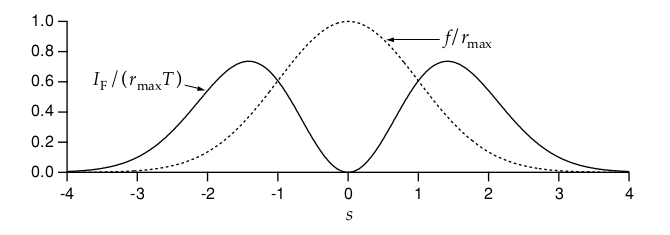
\includegraphics[scale = 0.4]{./png/3-11}
\end{center}
\end{exm}

\begin{rem}
  Individual neurons carry the most Fisher
information in regions of their tuning curves where average firing rates
are rapidly varying functions of the stimulus value, not where the firing
rate is highest.
\end{rem}
\begin{rem}
   The Fisher information can be used to derive an interesting result on the
optimal widths of response tuning curves. Consider a population of neurons with tuning curves of identical shapes, distributed evenly over a
range of stimulus values as in Example \ref{exm:Gaussian tuning curves}. Equation \ref{eq:3.45} indicates that the
Fisher information will be largest if the tuning curves of individual neurons are rapidly varying (making the square of their derivatives large), and
if many neurons respond (making the sum over neurons large). For typical neuronal response tuning curves, these two requirements are in conflict.
If the population of neurons has narrow tuning curves,
individual neural responses are rapidly varying functions of the stimulus,
but few neurons respond. Broad tuning curves allow many neurons to
respond, but the individual responses are not as sensitive to the stimulus
value.
\end{rem}
\begin{exm}
  To determine whether narrow or broad tuning curves produce the
more accurate encodings, we consider a dense distribution of Gaussian
tuning curves, all with $\sigma_a=\sigma_{r}$. Using such curves in
Equation \ref{eq:3.45}, we find
\begin{equation}
  \label{eq:3.46}
  I_{\rm{F}}(s)=T\sum\limits_{a=1}\limits^N
  {\frac{r_{\max}(s-s_{a})^{2}}{\sigma_r^{4}}\exp \left( -\frac{1}{2}\left( \frac{s-s_{a}}{\sigma_{r}} \right)^{2} \right)}.
\end{equation}
\end{exm}

\begin{prop}

This expression can be approximated by replacing the sum over neurons
with an integral over their preferred stimulus values and multiplying by a
density factor $\rho_{s}$. The factor $\rho_{s}$ is the density with which the neurons cover
the range of stimulus values, and it is equal to the number of neurons with
preferred stimulus values lying within a unit range of $s$ values. Replacing
the sum over $a$ with an integral over a continuous preferred stimulus parameter $\xi$ (which replaces $s_{a}$ ), we find
\begin{equation}
  \begin{aligned}
    \label{eq:3.47}
   I_{\rm{F}}(s)&=\rho_{s}T\int_{-\infty}^{\infty}{\frac{r_{\max}(s-\xi)^{2}}{\sigma_r^4}\exp\left(-\frac{1}{2}\left( \frac{s-\xi}{\sigma_r}\right)^{2} \right)}\\
                  &=\frac{\sqrt{2\pi}\rho_{s}\sigma_rr_{\max}T}{\sigma_r^2}.
  \end{aligned}
\end{equation}
The number of neurons that respond to a given stimulus value is
roughly $\rho_{s}\sigma_r$, and the Fisher information is proportional to this number divided by the square of the
tuning curve width seen from Equation \ref{eq:3.47}.Combining these factors, the Fisher information is inversely proportional to $\sigma_{r}$, and the encoding accuracy increases with narrower tuning curves.
\end{prop}

\begin{prop}
  Consider a stimulus with
$D$ parameters and suppose that the response tuning curves are products
of identical Gaussians for each of these parameters. If the tuning curves
cover the $D$-dimensional space of stimulus values with a uniform density $\rho_{s}$, the number of responding neurons for any stimulus value is proportional to $\rho_{s}\sigma_r^{D}$ and, using the same integral approximation as in equation (\ref{eq:3.47}), the Fisher information is
\begin{equation}
  I_{\rm{F}}=\frac{(2\pi)^{D/2}D\rho_{s}\sigma_r^{D}r_{\max}T}{\sigma_r^2}=(2\pi)^{D/2}D\rho_{s}\sigma_r^{D-2}r_{\max}T.
\end{equation}
\end{prop}

\begin{rem}
  The trade-off between the encoding accuracy of individual neurons and the
number of responding neurons depends on the dimension of the stimulus space. Narrowing the tuning curves (making $\sigma_{r}$ smaller) increases the
Fisher information for $D=1$, decreases it for $D > 2$, and has no impact if
$D = 2$.
\end{rem}

\subsection{Optimal Discrimination}
\begin{rem}
   In the first part of this chapter, we considered discrimination between two
values of a stimulus. An alternative to the procedures discussed there is
simply to decode the responses and discriminate on the basis of the estimated stimulus values.
\end{rem}
\begin{prop}
  Consider the case of discriminating between s
and $s+\Delta s$ for small $\Delta s$. For large $N$, the average value of the difference
between the ML estimates for the two stimulus values is equal to
$\Delta s$ (because the estimate is unbiased) and the variance of each estimate (for small
$\Delta s$) is $1/I_{\rm{F}}(s)$ . Thus, the discriminability, defined
in Equation \ref{eq:3.4}, for the ML-based test is
\begin{equation}
  \label{eq:3.49}
  d'=\Delta s \sqrt{I_{\rm{F}}(s)}.
\end{equation}
It can be known that the larger the Fisher information, the higher the discriminability.
\end{prop}

\begin{exc}
  Proof that for small $s$, this discriminability is the same
as that of the likelihood ratio test $Z(\mathbf{r})$ defined in Equation \ref{eq:3.47}.
\end{exc}



\begin{exm}
  The figure makes a comparison of Fisher information and discrimination thresholds for
orientation tuning.The solid curve is the minimum standard deviation of an estimate of orientation angle from the Cramér-Rao bound, plotted as a function of the
number of neurons $(N)$ involved in the estimation. The triangles are data points
from an experiment that determined the threshold for discrimination of
the orientation of line images by human subjects.
\begin{center}
   \includegraphics[scale = 0.6]{./png/3-12}
\end{center}
\end{exm}
















%%% Local Variables:
%%% mode: latex
%%% TeX-master: "../notesOnFluidMechanics"
%%% End:



\end{multicols}

%%% Local Variables:
%%% mode: latex
%%% TeX-master: "../notesOnFluidMechanics"
%%% End:



\clearpage

\appendix


%\bibliography{bib/numericalApprox}
%\bibliographystyle{abbrv}
%\bibliographystyle{abbrvnat}
%\setcitestyle{authoryear,open={[},close={]}}

\end{document}


%%% Local Variables: 
%%% mode: latex
%%% TeX-master: t
%%% End: 
